\documentclass[a4paper, 12pt]{./Template/lnls-note-PT}
\usepackage{amsmath}
\usepackage{amssymb}
\usepackage{amsthm}
\usepackage{indentfirst}
\numberwithin{equation}{section} %numera a equação de acordo com sua seção
\usepackage[pdftex,colorlinks=true,citecolor=black,linkcolor=black,urlcolor=black,filecolor=black]{hyperref}
\usepackage[num,abnt-emphasize=bf, bibjustif]{abntex2cite}
\usepackage{tipa}
\usepackage{ulem}
\usepackage{mathrsfs}
\citebrackets[]
%\documentclass[a4paper, 12pt, report]{lnls-note} % if you want to have chapters choose this one
\newcommand{\lambdabar}{\mbox{\textipa{\textcrlambda}}}
\def\mean#1{\left< #1 \right>}
%loads standard preamble configuration
%Standard preamble for documentation preparation

% \usepackage[T1]{fontenc}
% \usepackage{txfonts}
% \usepackage{authblk} % para varios autores em um mesmo artigo
\usepackage{graphicx}
\usepackage{subfigure}
\usepackage{fancyvrb} %fancy verbatim environment
\usepackage{amssymb}  % more symbols
% \usepackage{booktabs}
\usepackage{multirow} % enable multi row in tables
\usepackage{ulem}  % used to strike text
\usepackage{scrextend} % allow reference to footnotes
\usepackage[version=3]{mhchem} % Package for chemical equation typesetting
\usepackage{siunitx} % Package for units in SI
\usepackage{amsmath} % package with several mathematical symbols
% \usepackage{mathtools} % aligned environment inside align environment
% \usepackage[num]{abntcite}
\usepackage{lmodern} % carrega a fonte natural do latex com T1
\usepackage{textcomp} % package with symbols
\usepackage{floatrow}% Table float box with bottom caption, box width adjusted to content
\usepackage[hang,small]{caption}% legendas menores e o hang=alinha a legenda
\usepackage{hyperref} %possibilita o uso das refer�ncias e hiperlinks
\hypersetup{colorlinks,%
	    citecolor=black,%
	    filecolor=black,%
	    linkcolor=black,%
	    urlcolor=blue}
\usepackage{algpseudocode} %algorithmic package
\usepackage{algorithm}     % float environment for algorithm

%loads standard commands
\newcommand{\mc}[3]{\multicolumn{#1}{#2}{#3}} % multicolumns in a table
\newcommand{\mr}[3]{\multirow{#1}{#2}{#3}}    % multirows in a table
\newcommand{\deriva}[2]{\frac{\text{d} #1}{\text{d} #2}} % derivada de #1 em relacao a #2
\newcommand{\bit}{\begin{itemize}}
\newcommand{\eit}{\end{itemize}}
\newcommand{\bce}{\begin{center}}
\newcommand{\ece}{\end{center}}
\newcommand{\beq}{\begin{equation}}
\newcommand{\eeq}{\end{equation}}
\newcommand{\bfl}{\begin{flushleft}}
\newcommand{\efl}{\end{flushleft}}
\newcommand{\degre}{$^\circ$}% Changed this one because there already is a \degree macro in latex
\newcommand{\see}{$\rightarrow$}
\newcommand{\nmrad}{nm$\cdot$rad}
\newcommand{\powten}[1]{$\cdot 10^{#1}$}

\newcommand{\frage}[1]{~\\ \fbox{\small \tt #1}\\}




\begin{document}

\lnlstitle{134518}{\today}{Grupo de Estudos: Física de Aceleradores}
{Isabella Stevani}{\LNLS}
{Seguindo o livro \textit{The physics of electron storage rings: an introdution} de Matthew Sands \cite{sands1970physics}, este grupo de estudos tem por objetivo estudar e discutir o funcionamento de um acelerador de partículas, desde os elementos que o compõe como os fenômenos físicos que modelam sua dinâmica. Este documento traz anotações e deduções úteis de forma a facilitar o completo entendimento deste assunto.}

\newpage
\setcounter{page}{2}
\tableofcontents

\newpage
\section{Introdução}
	%\subsection{Comentários iniciais}
    \subsection{Mecanismos básicos}
Para facilitar o entendimento dos processos descritos a seguir, a Figura \ref{fig:ring} representa a estrutura física de um anel de armazenamento.
	
\begin{figure}[!htb]
	\centering
	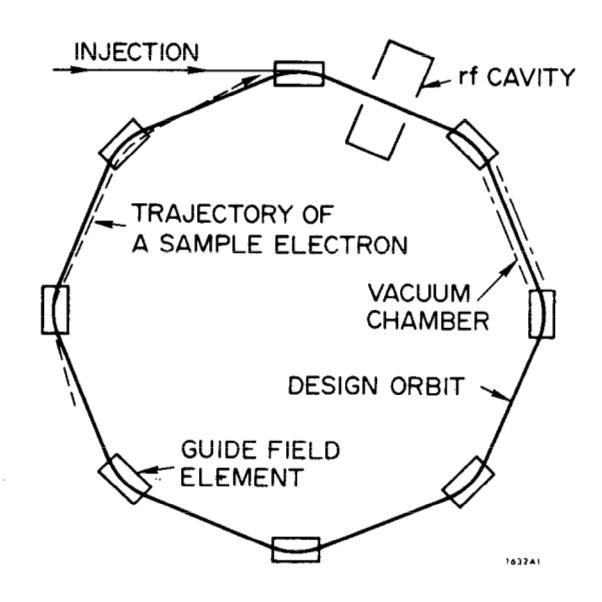
\includegraphics[width=0.6\linewidth]{./Figuras/fig1.jpeg}
	\caption{Diagrama esquemático de um anel de armazenamento de elétrons. Retirado de 						\cite{sands1970physics}.}
	\label{fig:ring}
\end{figure}
	
Um feixe de elétrons é injetado em uma câmara circular em vácuo. Campos magnetostáticos guiam as partículas pela câmara de vácuo. Tais campos são chamados de \emph{campos guia}. A interação eletromagnética entre o campo guia e os elétrons causa uma aceleração centrípeta do feixe, curvando assim sua trajetória e gerando um \emph{órbita fechada} desejada e desenhada a partir da escolha criteriosa do campo.
	
Esse campo guia, além de fechar a trajetória em uma órbita, tem propriedades focalizadoras que fazem com que cada elétron execute oscilações pseudo-harmônicas na transversal, as quais são chamadas de \emph{oscilações betatron}.
	
A cada volta, o elétron perde uma pequena parte da sua energia em forma de \emph{radiação síncrotron}. Esta energia perdida é reposta através de campos elétricos oscilantes no tempo gerados na \emph{cavidade de rádio frequência} (RF) e que aceleram longitudinalmente o feixe. Essas pequenas variações de perda e ganho da energia dos elétrons causam também oscilações no comprimento de órbita, no período de revolução, e ainda, no instante de chegada $\tau$ dos elétrons na cavidade de RF. As oscilações no plano energia-$\tau$ são chamadas de \emph{oscilações síncrotron} (ou oscilações de fase). Essas oscilações longitudinais dos elétrons são medidas em relação às \emph{partículas síncronas}, que são definidas como aqueles elétrons idealizados cujas energias, períodos de revolução e fase de chegada à cavidade de RF têm valores nominais.

Existem fases ideais de chegada à cavidade de RF em que o campo elétrico da cavidade é tal que a energia reposta por ele coincide com a energia média perdida pelos elétrons em cada volta. Cada uma destas fases ideais é chamada de \emph{fase síncrona}. O \emph{número harmônico} de um anel é definido como sendo a razão inteira entre a frequência de RF e a frequência de revolução dos elétrons. O número harmônico nos dá então o número de fases síncronas que podem ser acomodados no anel. Ao redor de cada uma destas fases síncronas, que são pontos fixos do espaço de fase energia-$tau$ nos quais se situam as partícula síncronas, pode-se ter uma distribuição de elétrons descrevendo oscilações síncrotron. Estas distribuições de elétrons em torno de das fases síncronas são chamadas de pacotes ou \emph{bunches}. Tipicamente o número harmônico dos anéis assume valor alto, permitindo assim um grande número de bunches e, em consequência, uma corrente de feixe circulante mais intensa.
	
A perda de energia por radiação síncrotron junto com a compensação gerada pela cavidade de RF causa um lento amortecimento da radiação de todas as amplitudes de oscilação, fazendo com que a trajetória de cada elétron tenda à trajetória do elétron de referência, o qual possui velocidade constante ao longo da órbita ideal.
	
Amortecimento da radiação não conserva o espaço de fase, então pode-se injetar vários \textit{bunches} no mesmo anel. O amortecimento de todas as amplitudes de oscilação é efetivamente preso devido à excitação contínua das oscilações por um "ruído" na energia do elétron, que vem do fato da radiação síncrona ser emitida em fótons de energia discreta. Este fenômeno é chamado de flutuação quântica da perda de energia. Em condições estacionárias, um equilíbrio é alcançado entre a excitação quântica e o amortecimento da radiação, levando a uma distribuição estatística estacionária das amplitudes e fases de oscilação dos elétrons em um \textit{bunch}. O \textit{bunch}, então, toma forma de uma tira elástica viajante, a qual tem tamanho e forma estacionários, com uma distribuição Gaussiana das amplitudes em cada coordenada transversal e longitudinal (Figura \ref{fig:fig2}). 
	
\begin{figure}[!htb]
	\centering
	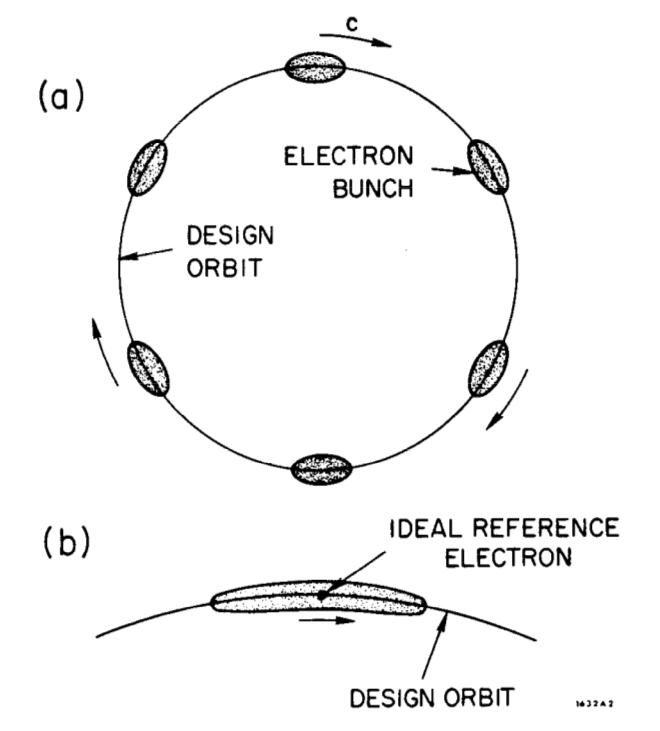
\includegraphics[width=0.55\linewidth]{./Figuras/fig2.jpeg}
	\caption{\textit{Bunches} circulando em um anel de armazenamento. Retirado de 							\cite{sands1970physics}.}
	\label{fig:fig2}
\end{figure}
	
Para cada coordenada do elétron, existe uma amplitude de oscilação máxima chamada de abertura dinâmica, a qual o elétron não fica mais preso dentro do \textit{bunch}. A abertura dinâmica para cada coordenada é definida por um obstáculo físico (tamanho da câmara de vácuo, por exemplo) ou por efeitos não-lineares nas forças focalizadoras, gerando trajetórias não-limitadas.
    \subsection{Efeitos coletivos}
Quando há um número suficientemente grande de elétrons em um \textit{bunch}, as interações entre os elétrons são relevantes (seja entre os elétrons ou entre os \textit{bunches}). 
	
\begin{itemize}
	\item \textit{Touschek-effect}. Dois elétrons oscilando em um \textit{bunch} podem transferir um pouco da sua energia de oscilação de uma coordenada transversal para uma longitudinal se sofrerem espalhamento de Coulomb. As novas amplitudes podem estar fora da aceitância em energia, ou aumentar o tamanho do \textit{bunch}. Esse efeito é relevante em baixas energias (menor que 1 GeV).
    \item Oscilações coerentes. Cada elétron no feixe produz campos eletromagnéticos na câmara de vácuo 	que influenciam o movimento dos outros elétrons. Estas interações coletivas podem gerar oscilações 		coerentes instáveis, em que todos os elétrons de um \textit{bunch} oscilam num modo coletivo em que 	a amplitude aumenta exponencialmente com o tempo. Estas oscilações coerentes envolvem tanto a 			dinâmica transversal quanto a longitudinal, podendo aumentar o tamanho do \textit{bunch} ou levar à 	perda de elétrons.
\end{itemize}
	
Interferência construtiva dos campos de radiação dos elétrons em um \textit{bunch} talvez gere radiação síncrona coerente, que pode aumentar a perda de energia de cada elétron individualmente. Este efeito não é considerado significante nos anéis de armazenamento mais novos.
	
Para conseguir a alta densidade de corrente desejada nos anéis de armazenamento, as instabilidades coerentes devem ser suprimidas ou controladas. Os outros efeitos coletivos são combinados com os efeitos individuais para determinar a dimensão do \textit{bunch}.
    \pagebreak
  
\section{Oscilações Betatron}\label{part2}
	\subsection{Sistema de coordenadas}
É conveniente utilizar um sistema de coordenadas cilíndrico para descrever a trajetória de um elétron dentro do anel de armazenamento (\autoref{fig:fig7}), uma vez que é desejado que seu movimento seja circular. Sendo assim, definem-se as coordenadas
\begin{itemize}
	\item $s$ -- Coordenada longitudinal, representa a distância entre um ponto de referência na órbita ideal e o ponto mais próximo do elétron nesta mesma órbita.
	\item $x$ e $z$ -- Coordenadas transversais, representam os deslocamentos horizontal e vertical com relação à órbita ideal, respectivamente.
\end{itemize}

\begin{figure}[!htb]
	\centering
	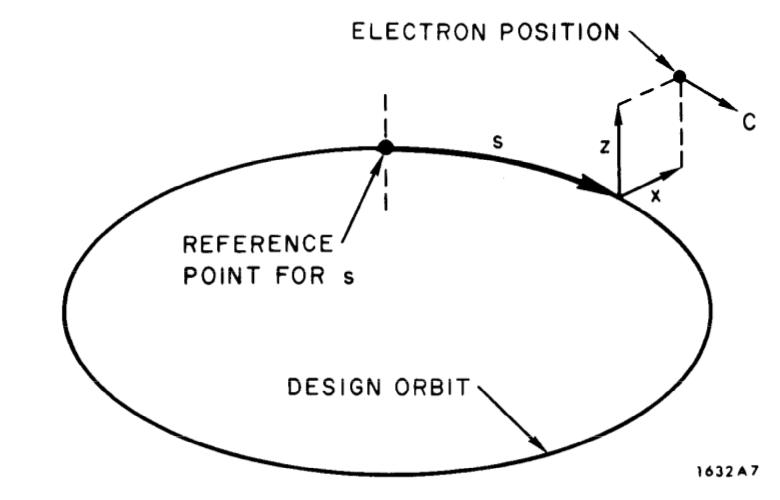
\includegraphics[width=0.6\linewidth]{./Figuras/fig7.jpeg}
	\caption{Coordenadas para descrever as trajetórias. Retirado de \cite{sands1970physics}.}
	\label{fig:fig7}
\end{figure}
    \subsection{Campo guia}\label{sec:2.2}
Pelo principio da inércia de Newton, um corpo tende a permanecer em movimento retilínio uniforme se não há forças que o obriguem a mudar sua trajetória. Logo, para que o elétron tenha uma órbita circular, é necessário aplicar uma força que mude sua trajetória da forma desejada.

Pela força de Lorentz,
\begin{align}
	\vec{F} = q\left(\vec{E} + \vec{v} \times \vec{B}\right)
\end{align}
onde $q$ é a carga da partícula em movimento, $\vec{E}$ é o vetor de campo elétrico, $\vec{v}$ é o vetor de velocidade da partícula e $\vec{B}$ é o vetor de campo magnético.

A contribuição referente à força elétrica ($q\vec{E}$) é paralela ao campo elétrico, enquanto a contribuição referente à força magnética ($q(\vec{v}\times\vec{B})$) é perpendicular ao campo magnético e à velocidade. Devido a este fato, a força magnética não realiza trabalho, uma vez que é perpendicular ao deslocamento da partícula. Logo, a força magnética altera a direção do vetor velocidade -- e, por consequência, do movimento da partícula -- sem alterar o seu módulo. Apenas a força elétrica pode realizar trabalho.

Desta forma, a fim de desviar a partícula da sua trajetória, aplica-se um campo magnético $\vec{B}$ nos pontos onde ela deve fazer alguma curva, o qual é chamado de campo guia. Com $E=0$,
\begin{align}
	\vec{F} = q\vec{v}\times\vec{B}
\end{align}

Espera-se que a órbita ideal ocorra no plano horizontal ($z=0$) de forma que o campo magnético deve ser puramente vertical em toda a órbita do anel. Considerando o campo magnético simétrico com relação ao plano da órbita ideal e fazendo uma aproximação linear, pode-se escrever a equação do campo magnético através da expansão de Taylor:
\begin{align}
	B_z(s,x,z) &= B_0(s) + \left(\frac{\partial B_z}{\partial x}\right)_{0s} x\label{eq:2.01}\\
	B_x(s,x,z) &= \left(\frac{\partial B_x}{\partial z}\right)_{0s} z\label{eq:2.02}
\end{align}

Pela simetria imposta, aplicando as leis de Maxwell,
\begin{align}
	\frac{\partial B_z}{\partial x} = \frac{\partial B_x}{\partial z}
\end{align}

Desta forma, as equações \eqref{eq:2.01} e \eqref{eq:2.02} podem ser reescritas como
\begin{align}
	B_z(s,x,z) &= B_0(s) + \left(\frac{\partial B}{\partial x}\right)_{0s} x\label{eq:2.1}\\
	B_x(s,x,z) &= \left(\frac{\partial B}{\partial x}\right)_{0s} z\label{eq:2.2}
\end{align}

Como o campo é simétrico em relação ao plano da órbita ideal, as variáveis $B_0$ e $\frac{\partial B}{\partial x}$ possuem apenas componentes verticais, então apenas suas magnitudes são necessárias para descrevê-las completamente e os índices $s$ e $z$ podem ser suprimidos.

Anéis de armazenamento são modelados para operar em uma faixa de valores de energia dos elétrons. Isto é obtido arranjando de forma que os campos magnéticos possam ser variados juntos -- sendo parametrizados proporcionalmente à energia de operação desejada. Claramente, se o campo magnético na órbita ideal é mudado em todo o anel pelo mesmo fator, a órbita ideal será, novamente, uma trajetória possível de um elétron cujo momento é mudado pelo mesmo fator. Variar todos os campos juntos altera muito pouco a energia associada com a órbita ideal. Por essas razões, é conveniente especificar as propriedades do campo guia de uma maneira que seja independente de qualquer energia de operação escolhida, o que é facilmente feito dividindo todos os campos por um fator proporcional à energia associada do elétron, o qual é chamado de rigidez magnética. Desta forma, as propriedades lineares do campo guia podem ser definidas pelas funções
\begin{align}
	G(s) &= \frac{ecB_0(s)}{E_0}\label{eq:2.3}\\
	K_1(s) &= \frac{ec}{E_0} \left(\frac{\partial B}{\partial x}\right)_{0s}
\end{align}
onde $E_0$ é a energia nominal, $c$ é a velocidade da luz e $e$ é a carga do elétron. Note que estas funções tem um significado físico bem simples. Neste caso, apenas elétrons ultra-relativísticos são considerados, então sua energia é dada por $E=cp$. Desta forma, $G(s)$ é apenas o inverso do raio de curvatura $\varrho(s)$ dos elétrons em $x=0$ e $z=0$ com energia nominal, ou seja,
\begin{align}
	G(s) = \frac{1}{\varrho(s)}
\end{align}

\begin{proof}
	Como a partícula está rotacionando sobre ação da força de Lorentz, esta força deve ser equivalente a sua força centrípeta. Logo,
	\begin{align*}
		\frac{mv^2}{\varrho(s)} &= q\vec{v}\times\vec{B}\\
							    &= evB_0(s)\\
	\end{align*}
	
	Como o elétron é ultra-relativístico (com velocidade próxima/igual à velocidade da luz), a energia da partícula é dada por
	\begin{align*}
		E_0^2 = (m_0 c^2)^2 + p^2c^2
	\end{align*}
	onde $m_0$ é a massa de repouso e $p$ o momento da partícula. Pelo mesmo argumento anterior, $(m_0c^2)^2 << c^2p^2$. Desta forma, pode desprezar o termo $(m_0c^2)^2$ e a energia da partícula é dada por
	
	\begin{align*}
		E_0 &= pc\\
			&= \gamma m_0 c^2\\
			&= mc^2
	\end{align*}
	
	Substituindo,
	\begin{align*}
			\frac{mv^2}{\varrho(s)} &= ecB_0(s)\\
			\frac{E_0}{\varrho(s)} &= ecB_0(s)\\
			\therefore \frac{1}{\varrho(s)} &= \frac{ecB_0(s)}{E_0} = G(s)
	\end{align*}
	
	Desta forma, reescrevendo a equação do campo magnético em função de $G(s)$,
	\begin{align*}
		B_z(s,x,z) &= B_0(s) + \frac{\partial B}{\partial x} x\\
				   &= \frac{E_0}{ec} G(s) + \frac{\partial B}{\partial x} x
	\end{align*}
	
	Definindo a função $K_1(s)$ como
	\begin{align*}
		K_1(s) = \frac{ec}{E_0} \frac{\partial B}{\partial x}
	\end{align*}
	tem-se que
	\begin{align*}
		B_z(s,x,z) &= \frac{E_0}{ec} G(s) + \frac{\partial B}{\partial x} x\\
				   &= \frac{E_0}{ec} G(s) + \frac{E_0}{ec} K_1(s) x\\
				   &= \frac{E_0}{ec} [G(s) + K_1(s) x]
	\end{align*}
	Reescrevendo $B_x(s,x,z)$ da mesma forma, as equações do campo magnético são
	\begin{align*}
		B_z(s,x,z) &= \frac{E_0}{ec} [G(s) + K_1(s) x]\\
		B_x(s,x,z) &= \frac{E_0}{ec} K_1(s) z
	\end{align*}
\end{proof}

A constante de proporcionalidade $\frac{E_0}{ec}$ é a rigidez magnética do anel de armazenamento. Ela normaliza as equações do campo magnético de forma que este dependa apenas das propriedades da ótica do anel.

Devido à relação entre $G(s)$ e $\varrho(s)$, $G(s)$ é chamada de função de curvatura. A função $K_1(s)$ é a taxa de variação do raio inverso com o deslocamento radial.

As funções $G(s)$ e $K_1(s)$ podem ser arbitrárias, porém devem satisfazer alguns requisitos importantes. Primeiro, $G(s)$ precisa ser tal que esta defina uma órbita fechada (pode-se pensar que $G(s)$ define a órbita ideal, ou que alguma órbita fechada arbitrária define $G(s)$ de forma única). A variação $d \theta_0$ na direção da tangente à órbita ideal em um intervalo $ds$ é
\begin{align}
	-d\theta_0 = \frac{ds}{\varrho(s)} = G(s)ds
\end{align}

O ângulo percorrido em uma revolução precisa ser igual a $2\pi$, então $G(s)$ deve satisfazer
\begin{align}
	\int_{0}^{L} G(s)ds = 2\pi
\end{align}

Segundo, tanto $G(s)$ quanto $K_1(s)$ são, necessariamente, funções periódicas de $s$, devido ao fato de que a coordenada longitudinal $s$ é fisicamente cíclica -- retornando ao mesmo ponto da órbita após uma revolução. Dito isso, $G(s)$ e $K_1(s)$ também devem satisfazer
\begin{align}
	\left\{\begin{array}{rcl}
	\ G(s+L) & = & G(s)\\
	K_1(s+L) & = & K_1(s)
	\end{array}\right.
\end{align}
onde $L$ é o comprimento da órbita. Execeto por estas condições, $G(s)$ e $K_1(s)$ podem ter mais ou menos variações arbitrárias com $s$.

Apesar das funções do campo guia $G$ e $K_1$ serem, a princípio, bem gerais, geralmente é conveniente simplificar o design ou a operação de um anel de armazenamento impondo certas restrições nestes aspectos. Por exemplo, a maioria dos anéis de armazenamento são desenhados para ter o mesmo raio de curvatura, diga-se $\varrho_0$, em todos os ímãs de curvatura -- e sem nenhuma curvatura entre um ímã e outro, ou seja, apenas trechos retos. Este tipo de campo guia é chamado isomagnético. O intuito desta configuração é que o campo magnético sobre a órbita ideal tenha o mesmo valor em todo lugar, exceto onde este é nulo. Então $G(s)$ é uma função dicotômica:
\begin{align}
	G(s) = \left\{\begin{array}{rrrr}
	\ G_0 & = & \frac{1}{\varrho_0}, &  no\ \acute{i}m\tilde{a}\\
	0, & & & em\ todo\ o\ resto
	\end{array}\right.
\end{align}

Um campo guia real não pode, claro, ser idealmente isomagnético, já que é fisicamente impossível ter um campo magnético descontínuo. Sempre há uma zona de transição nas bordas do ímã onde o campo vai de zero ao seu valor nominal. A aproximação isomagnética ideal é, entretanto, um tanto quanto adequada no geral.

Apesar de aceleradores e anéis de armazenamento comumente serem construídos com ímãs de curvatura com gradientes radiais de campo, é comum desenvolver campos guia de função separável, ou seja, campos magnéticos em que as funções de focalização e curvatura são atribuídas a elementos magnéticos diferentes. Isto é, o campo guia consiste numa sequência de dipolos (sem gradiente de campo) e quadrupolos (sem campo na órbita ideal). Pensando nesta configuração, define-se um campo guia de função separável onde as funções $G(s)$ e $K_1(s)$ devem satisfazer a condição
\begin{align}
	G(s)K_1(s) = 0\label{eq:2.10}
\end{align}

Um pouco de atenção para este fato. Às vezes é conveniente projetar os ímãs de curvatura com faces retangulares. Com este tipo de ímã, a órbita ideal deve entrar ou sair do ímã com um ângulo diferente de 90$^\circ$ em relação à borda do mesmo (Figura \ref{fig:fig8}). Mesmo que o ímã seja plano (sem gradiente radial no ímã), irão existir gradientes radiais nas bordas, onde o campo não é nulo. A equação \eqref{eq:2.10} não é satisfeita nas bordas, e um campo guia construído com estes ímãs retangulares -- junto com os quadrupolos -- não irá satisfazer a definição de função separável, mesmo que ele seja referenciado como tal às vezes. Estes campos ainda podem ser, entretanto, isomagnéticos. 

\begin{figure}[!htb]
	\centering
	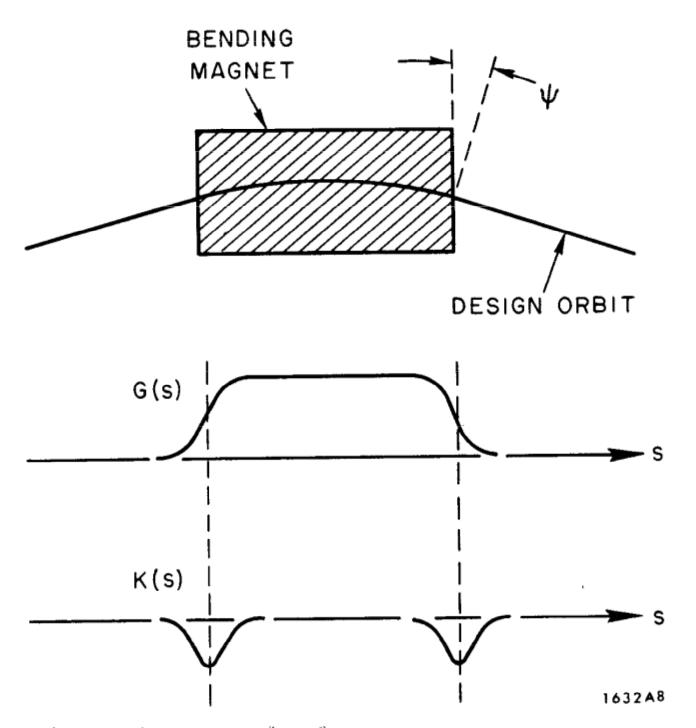
\includegraphics[width=0.6\linewidth]{./Figuras/fig8.jpeg}
	\caption{Campo guia com ímã retangular. Retirado de \cite{sands1970physics}.}
	\label{fig:fig8}
\end{figure}
    \subsection{Equações de movimento}\label{sec:2.3}
As equações de movimento descrevem a trajetória de um elétron se movendo próximo da órbita ideal, com uma energia próxima, mas não necessariamente igual, à energia nominal $E_0$. O desvio de energia é definido como
\begin{align}
	\epsilon = E-E_0
\end{align}
onde $E$ é a energia do elétron.

Para manter a aproximação linear, são considerados apenas pequenas quantidades de $x$, $z$ e $\epsilon$. Melhor do que tomar o tempo como variável independente, é mais conveniente adotar a coordenada longitudinal $s$. Assim, derivadas com relação a $s$ serão indicadas daqui pra frente pela notação $(')$. Por exemplo, $x'=\frac{dx}{ds}$.

Começando a análise pelo movimento radial. Considere um elétron em $x$ movendo-se com inclinação $x'$ (Figura \ref{fig:fig9}). A inclinação é o ângulo entre a direção do movimento do elétron e a tangente à órbita ideal. $x'$ é o ângulo entre a trajetória e a tangente à órbita ideal. Suponha um ângulo $\theta_0$ entre a tangente e uma direção de referência arbitrária e um ângulo $\theta$ entre a trajetória e a mesma direção de referência. Logo, $x' = \theta-\theta_0$ e
\begin{align}
	x'' = \frac{d(\theta-\theta_0)}{ds}\label{eq:2.12}
\end{align}

\begin{figure}[!htb]
	\centering
	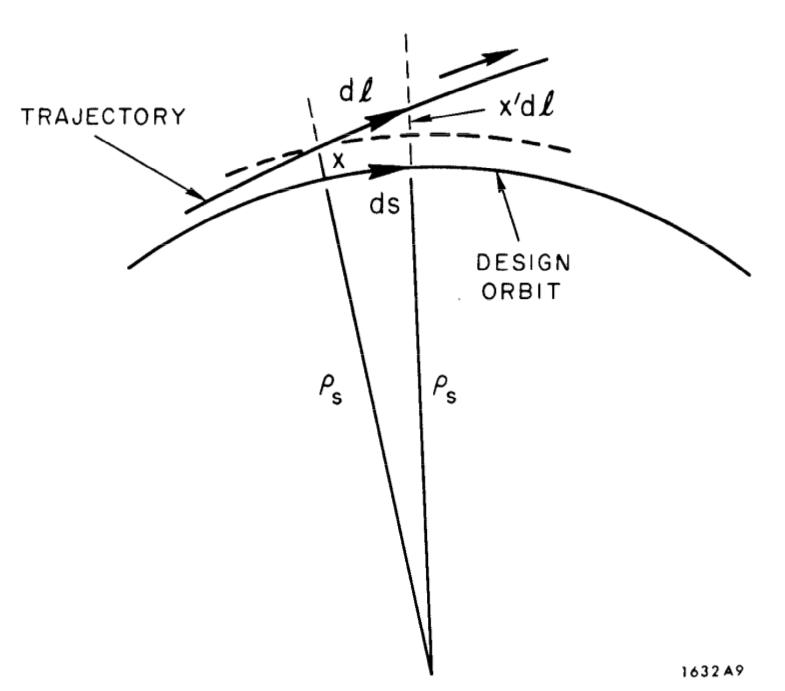
\includegraphics[width=0.6\linewidth]{./Figuras/fig9.jpeg}
	\caption{Trajetória de um elétron próxima à órbita ideal. Retirado de \cite{sands1970physics}.}
	\label{fig:fig9}
\end{figure}

A derivada de $\theta_0$ é, como já foi visto, $\frac{-1}{\varrho_s} = G(s)$ ($\varrho_s = \varrho(s)$). Mas o que é $\frac{d\theta}{ds}$? O rario de curvatura da trajetória é
\begin{align}
	\varrho = \frac{E}{ecB}
\end{align}
e, em um elemento de caminho $d\ell$ da trajetória, a variação do ângulo é
\begin{align}
	d\theta = -\frac{d\ell}{\varrho} = -\frac{ecB}{E}d\ell\label{eq:2.14}
\end{align}

Note que, enquanto o ângulo $x'$ é pequeno -- e pode-se sempre assumir isto desde que apenas termos de primeira ordem sejam considerados, que é o caso -- um elemento de caminho $d\ell$ da trajetória em $x$ é relacionado com a correspondente variação em $s$ por
\begin{align}
	d\ell = \frac{\varrho_s - x}{\varrho_s} ds = \left(1+\frac{x}{\varrho_s}\right)ds = (1+G(s))ds\label{eq:2.15}
\end{align}

Agora, $B$ pode ser descrito por
\begin{align}
	B = B_0 + \frac{\partial B}{\partial x}x = \frac{E_0}{ec}(G+K_1x)\label{eq:2.16}
\end{align}

Substituindo as equações \eqref{eq:2.15} e \eqref{eq:2.16} na equação \eqref{eq:2.14} juntamente com $E_0+\epsilon$ para $E$ -- e mantendo apenas termos de primeira ordem -- tem-se que
\begin{align}
	d\theta = \left\{-G-(G^2+K_1)x + G\frac{\epsilon}{E_0}\right\}ds
\end{align}
e, portanto, 
\begin{align}
	x'' = -(G^ 2+K_1)x + G\frac{\epsilon}{E_0}
\end{align}

\begin{proof}
	Pela equação \eqref{eq:2.14},
	\begin{align*}
		d\theta &= -\frac{ecB}{E}d\ell\\
				&= -\frac{ecB}{E}(1+Gx)ds\\
				&= -\frac{ec}{E}\left[\frac{E_0}{ec}(G+K_1x)\right](1+Gx)ds\\
				&= -\frac{E_0}{E_0+\epsilon}(G+K_1x)(1+Gx)ds\\
				&= -\frac{E_0}{E_0+\epsilon}(G+K_1x+G^2x+K_1Gx^2)ds\\
				&= -\frac{E_0}{E_0+\epsilon}(G+(G^2+K_1)x + K_1Gx^2)ds
	\end{align*}
	
	Mantendo apenas termos de primeira ordem para continuar com a aproximação linear,
	\begin{align*}
		d\theta &= -\frac{E_0}{E_0+\epsilon}(G+(G^2+K_1)x)ds\\
				&= \frac{E_0}{E_0+\epsilon}(-G-(G^2+K_1)x)ds\\
				&= \frac{1}{1+\epsilon/E_0}(-G-(G^2+K_1)x)ds\\
	\end{align*}
	
	Como $\epsilon/E_0$ é bem pequeno, pode-se considerar que o termo $\frac{1}{1+\epsilon/E_0}$ é a soma de uma série geométrica. Logo, pode-se expandir este termo em um somatório:
	\begin{align*}
		d\theta &= \left(1 - \frac{\epsilon}{E_0} + \frac{\epsilon^2}{E_0^2}+ ...\right)(-G-(G^2+K_1)x)ds
	\end{align*}
	
	Novamente, mantendo apenas termos de primeira ordem,
	\begin{align*}
		d\theta &= \left(1 - \frac{\epsilon}{E_0}\right)(-G-(G^2+K_1)x)ds\\
				&= (-G-(G^2+K_1)x)ds + \left(G\left(\frac{\epsilon}{E_0}\right)+(G^2+K_1)x\left(\frac{\epsilon}{E_0}\right)\right)ds
	\end{align*}
	
	Aplicando novamente o argumento acima,
	\begin{align*}
		d\theta = \left\{-G-(G^2+K_1)x + G\frac{\epsilon}{E_0}\right\}ds
	\end{align*}
	
	Agora, pela equação \eqref{eq:2.12},
	\begin{align*}
		x'' &= \frac{d(\theta-\theta_0)}{ds}\\
			&= \frac{\left\{-G-(G^2+K_1)x + G\frac{\epsilon}{E_0}\right\}ds - (-G)ds}{ds}\\
			&= -(G^2+K_1)x + G\frac{\epsilon}{E_0}
	\end{align*}
\end{proof}

A equação correspondente para o movimento vertical é
\begin{align}
	z'' = K_1 z
\end{align}

\begin{proof}
	Para $z''$, pela força de Lorentz,
	\begin{align*}
		d\theta &= -\frac{d\ell}{\varrho} = + \frac{ecB}{E}d\ell\\
				&= \frac{ecB}{E}d\ell\\
				&= \frac{ecB}{E}(1+Gx)ds\\
				&= K_1 z (1+Gx)ds\\
				& = (K_1 z + GK_1xz)ds
	\end{align*}
	
	Descartando o termo de segunda ordem,
	\begin{align*}
		d\theta &= K_1 z ds\\
	\end{align*}
	
	Agora, pela equação \eqref{eq:2.12},
	\begin{align*}
		z'' &= \frac{d(\theta-\theta_0)}{ds}\\
			&= \frac{K_1 z\ ds}{ds}\\
			&= K_1 z
	\end{align*}
	lembrando que $\frac{d\theta_0}{ds} = 0$ porque não há componente vertical nesta variação.
\end{proof}

Definindo as funções focalizadoras $K_x$ e $K_z$ como
\begin{align}
	K_x(s) &= G^2(s)+K_1(s)\label{eq:2.21}\\
	K_z(s) &= - K_1(s)
\end{align}
tem-se que $x''$ e $z''$ podem ser descritos como
\begin{align}
	x'' &= -K_x(s)x + G(s)\frac{\epsilon}{E_0}\label{eq:2.19}\\
	z'' &= -K_z(s)z\label{eq:2.20}
\end{align}

O termo correspondente à $G^2$ está "faltando" de $K_z$ devido à consideração de que a órbita ideal está no plano, ou seja, não possui componente vertical. Mais especificamente, $G^2$ é um termo de força centrífuga, e um termo correspondente apareceria no movimento vertical se a órbita tivesse picos e vales. Anéis de armazenamento possuem, em geral, uma forte focalização. Neste caso, $G^2$ é bem menor que $K_1$, então $K_x$ e $K_z$ são aproximadamente iguais e possuem sinais opostos. Fisicamente, esta diferença de sinal significa que um elemento focalizador que focaliza em $x$ automaticamente desfocaliza em $z$, e vice-versa.

A equação de movimento em $z$ parece a equação de uma oscilação clássica (força proporcional ao desvio), com um coeficiente de força restauradora variável -- a função $K_z(s)$. A equação em $x$ é similar, exceto pela adição de um termo variável proporcional ao desvio de energia $\epsilon$. Nos campos guia que podem ser efetivamente utilizados, as soluções destas equações são, na verdade, oscilatórias, e descrevem oscilações laterais -- incluindo as chamadas oscilações betatron -- na trajetória do elétron. Estas oscilações são resultado das propriedades focalizadoras do campo guia, as quais caracterizam as funções de focalização $K_x$ e $K_z$.

Tanto $K_x$ quanto $K_z$ são funções periódicas ao longo do anel, logo
\begin{align}
	\begin{array}{rcl}
	\ K(s+L) & = & K(s)
	\end{array}
\end{align}

Por conveniência na construção e no design do anel, este possui uma periodicidade intrínseca. Ou seja, é composta por uma sequência de células magnéticas idênticas, cada célula sendo constituída por dipolos e quadrupolos. Então, para um anel com células de comprimento $\ell_c$,
\begin{align}
	\left\{\begin{array}{rcl}
	\ G(s+\ell_c) & = & G(s)\\
	K(s+\ell_c) & = & K_1(s)
	\end{array}\right.
\end{align}

Nota-se que, diferentemente da primeira propriedade, a periodicidade de célula é uma propriedade do design da máquina, não sendo totalmente verdadeira em campos reais devido a imperfeições na construção.

Na \autoref{fig:fig10}, a natureza das funções de focalização em uma parte do anel, abrangendo duas células. A Figura \ref{fig:fig10} (a) mostra o configuração dos dipolos e quadrupolos do anel. Os dipolos são denominados por B e tem um campo uniforme ($dB/dx = 0$). Os quadrupolos não tem campo na órbita ideal ($B_0=0$) e são denominados por F e D (F para focalizador e D para desfocalizador, ambos com relação ao movimento radial). As Figuras \ref{fig:fig10} (b) e (c) são as funções de focalização $G$, $K_x$ e $K_z$.

\begin{figure}[!htb]
	\centering
	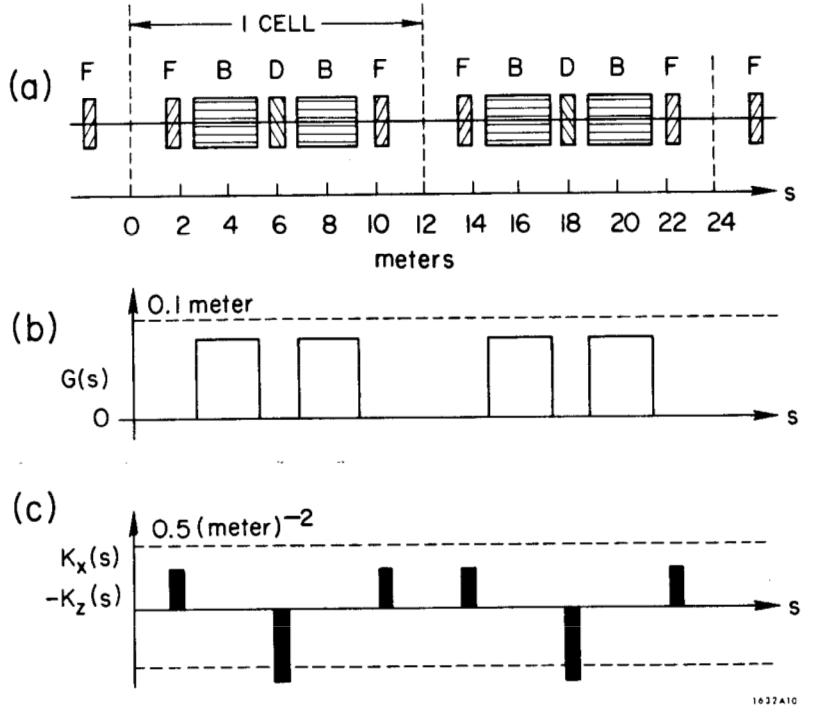
\includegraphics[width=0.7\linewidth]{./Figuras/fig10.jpeg}
	\caption{Laço magnético e funções de focalização em uma célula de um campo guia em particular. Retirado de \cite{sands1970physics}.}
	\label{fig:fig10}
\end{figure}
    \subsection{Separação do movimento radial}
É conveniente separar o movimento radial em duas partes: uma parte sendo uma curva fechada deslocada da órbita de design -- a órbita de equilíbrio dos elétrons com desvio de energia -- e a outra parte sendo a oscilação transversal em torno desta órbita. Suponha que $x$ seja
	
\begin{align}
	x = x_{\epsilon} + x_{\beta}\label{eq:2.25}
\end{align}
então certamente a equação \eqref{eq:2.19} é satisfeita se as equações
\begin{align}
	x_\epsilon'' &= -K_x(s)x_\epsilon + G(s)\frac{\epsilon}{E_0}\label{eq:2.26}\\
	x_\beta'' &= -K_x(s)x_\beta\label{eq:2.27}
\end{align}
forem verdadeiras.
	
\begin{proof}
    Pela equação \eqref{eq:2.25}, $x = x_{\epsilon} + x_{\beta}$. Logo,
    \begin{align*}
        x'' &= x_{\epsilon}'' + x_{\beta}''\\
            &= -K_x(s)x_\epsilon + G(s)\frac{\epsilon}{E_0} + K_x(s)x_\beta\\
            &= -K_x(s)(x_\epsilon + x_\beta) + G(s)\frac{\epsilon}{E_0}\\
            &= -K_x(s)x + G(s)\frac{\epsilon}{E_0}
    \end{align*}
\end{proof}
	
Definindo que $x_\epsilon(s)$ é uma função periódica em $s$ com período $L$, então $x_\epsilon(s)$ é a órbita fechada de um elétron com energia $E_0 + \epsilon$ (com $x_\beta=0$), e o movimento radial será a soma do desvio dessa nova órbita de equilíbrio e uma oscilação betatron.
	
O desvio $x_\epsilon$ é proporcional ao desvio de energia $\epsilon$. Define-se	
\begin{align}
	x_\epsilon(s) = \eta(s)\frac{\epsilon}{E_0}\label{eq:2.29}
\end{align}
onde $\eta(s)$ é a função única que satisfaz	
\begin{align}
	\begin{cases}
		\eta'' = -K_x(s)\eta + G(s), \\
        \eta(0) = \eta(L), \\
        \eta'(0) = \eta'(L).
    \end{cases}
\end{align}
	
\begin{proof}
	Seja $x_\epsilon(s)$ dado pela equação \eqref{eq:2.29}. Pela equação \eqref{eq:2.26},
	\begin{align*}
        x_\epsilon'' &= -K_x(s)x_\epsilon + G(s)\frac{\epsilon}{E_0}\\
        \left(\eta(s)\frac{\epsilon}{E_0}\right)'' &= -K_x(s)\eta(s)\frac{\epsilon}{E_0} + G(s)\frac{\epsilon}{E_0}\\
        \eta(s)''\frac{\epsilon}{E_0} &= -K_x(s)\eta(s)\frac{\epsilon}{E_0} + G(s)\frac{\epsilon}{E_0}\\
        \eta'' &= -K_x(s)\eta + G(s)
	\end{align*}
\end{proof}
	
Denomina-se $\eta(s)$ como sendo a função de órbita fechada, e é uma função que caracteriza o campo guia total do anel. Note que $\eta (s)$ é a solução particular da equação diferencial \eqref{eq:2.26} em que a função é periódica com período $L$ e não depende de características do elétron, apenas da ótica do anel.
    \subsection{Trajetórias betatron}\label{sec:2.5}
As equações \eqref{eq:2.20} e \eqref{eq:2.27} descrevem as oscilações betatron vertical e radial, respectivamente. Considerando as aproximações feitas, o movimento em cada coordenada é independente. Logo, como $K_x(s)$ e $K_z(s)$ tem a mesma forma matemática, toma-se a forma representativa
	
\begin{align}
	x'' = -K(s) \; x \label{eq:2.31}
\end{align}
	
Lembrando que $K_x(s)$ descreve a oscilação betatron radial de um elétron com energia nominal $E_0$ e $K_z(s)$ descreve o movimento vertical.
	
A função de focalização $K(s)$ é definida em cada coordenada $s$ pelo design do anel de armazenamento. Se a posição e a inclinação ($x$ e $x'$) são dadas em alguma coordenada $s$, os termos subsequentes podem ser obtidos integrando a equação \eqref{eq:2.31}. Porém, como o campo guia é construído de segmentos magnéticos e $K(s)$ pode ser considerada constante nestes intervalos, pode-se integrar $x$ e $x'$ para cada segmento e juntar estes resultados. Dependendo do valor de $K$, $x$ é dado por

\begin{align}
	\left\{\begin{array}{l}
	K>0: \ \ x = a\ \cos(\sqrt{K}s+b) \\
	K=0: \ \ x = as+b \\
	K<0: \ \ x = a\ \cosh(\sqrt{-K}s+b)
	\end{array}\right. \label{eq:2.32}
\end{align}
onde $a$ e $b$ são constantes em cada segmento e podem ser determinadas pelos valores de $x$ e $x'$ na entrada do segmento (como $K$ é finita em qualquer ponto, $x$ e $x'$ devem ser ambas contínuas em todo ponto -- em particular, na junção entre dois segmentos).
	
\begin{proof}
	A equação \eqref{eq:2.31} é uma equação diferencial homogênea de 2ª ordem. Considerando que a função $K$ é uma constante, supõe-se que a solução da EDO é uma exponencial, 		ou seja, da forma $x=e^{rs}$. Substituindo esta possível solução, tem-se
	\begin{align*}
		x'' + Kx &=0\\
		(e^{rs})'' + K(e^{rs}) &= 0\\
		r^2e^{rs} + Ke^{rs}&=0\\
		(r^2 + K)e^{rs} &=0\\
		e^{rs} \neq 0 \therefore r^2 + K &= 0
	\end{align*}
	
	A equação $r^2 + K = 0$ é a equação característica da EDO. Resolvendo-a, tem-se $r = \pm \sqrt{-K}$, então $x_{1,2} = e^{\pm\sqrt{-K}s}$. Agora, existem 3 casos possíveis:
	\begin{itemize}
		\item $K>0$\\
			
		Com $K<0$, as raízes da equação característica são imaginárias. A solução geral da EDO é, para este caso, $x = c_1e^{\alpha s}\cos(\beta s) + c_2e^{\alpha s}\sin(\beta s)$. Como a função seno é apenas a função cosseno com uma diferença de fase, pode-se escrever
        \begin{align*}
        	x = a \ \cos(\sqrt{K}+b)
        \end{align*}
			
		\item $K = 0$\\
		
		A solução geral da EDO é, para este caso, $x = c_1e^{\sqrt{K}s} + sc_2e^{-\sqrt{K}s}$. Como $K=0$, 
		\begin{align*}
            x &= c_1e^{\sqrt{K}s} + sc_2e^{\sqrt{K}s}\\
            x &= c_1e^{0s} + sc_2e^{0s}\\
            x &= c_1 + sc_2
		\end{align*}
		
		Renomeando as constantes, $x = as + b$.

		\item $K < 0$\\
				
		A solução geral da EDO é, para este caso, $x = c_1e^{\sqrt{-K}s} + c_2e^{-\sqrt{-K}s}$. Fazendo $c_1=c_2=\frac{1}{2}$,
		\begin{align*}
            x &= c_1e^{\sqrt{-K}s} + c_2e^{-\sqrt{-K}s}\\
            x &= \frac{e^{\sqrt{-K}s} + e^{-\sqrt{-K}s}}{2} = cosh(\sqrt{-K}x)
		\end{align*}
				
		Para constantes $c_1$ e $c_2$ arbitrárias,
		\begin{align*}
          x = a \ cosh(\sqrt{-K}x + b)
		\end{align*}
	\end{itemize}
	
	Concluindo,
	\begin{align*}
        \left\{\begin{array}{l}
        K>0: \ \ x = a\ \cos(\sqrt{K}s+b) \\
        K=0: \ \ x = as+b \\
        K<0: \ \ x = a\ \cosh(\sqrt{-K}s+b)
        \end{array}\right.
	\end{align*}
\end{proof}

Como ilustração, supõe-se uma funçãoi $K(s)$ como a função $K_x(s)$ na \autoref{fig:fig10}. Duas possíveis trajetórias estão representadas na \autoref{fig:fig11} (b). A primeira é a trajetória que começa em $s_0$ com deslocamento unitário $x_0=1$ e nenhuma inclinação $x_0'=0$. A segunda começa com deslocamento nulo $x_0=0$ e inclinação unitária $x_0'= 1$. A primeira é chamada de \textit{cosinelike trajectory} -- $C$ e a segunda de \textit{sinelike trajectory} -- $S$. Seus detalhes dependem da coordenada de referência $s_0$ e são, em geral, funções não periódicas, mesmo que $K(s)$ seja. Para um anel com trajetórias estáveis, $C$ e $S$ são funções oscilatórias limitadas as quais possuem uma forma diferente a cada revolução.

\begin{figure}[!htb]
	\centering
	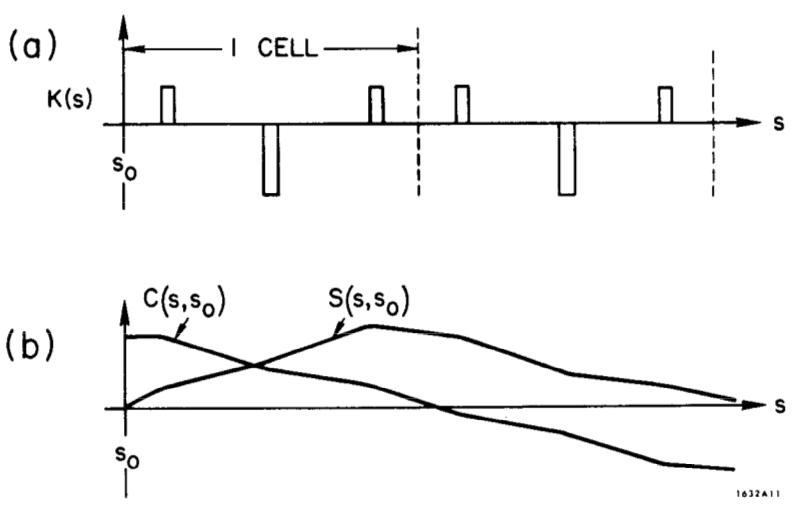
\includegraphics[width=0.7\linewidth]{./Figuras/fig11.jpeg}
	\caption{Função de focalização $K(s)$ e duas trajetórias: a \textit{cosine-like trajectory} e a \textit{sine-like trajectory} para uma coordenada de início $s_0 $. Retirado de \cite{sands1970physics}.}
	\label{fig:fig11}
\end{figure}
	
Agora, como a equação \eqref{eq:2.31} é linear em $x$, qualquer combinação linear de $C$ e $S$ também descreve uma trajetória possível para $x$. Mais que isso, qualquer trajetória pode ser descrita por esta combinação linear. Ou seja,
	
\begin{align}
	x(s) &= C(s,s_0)x_0 + S(s,s_0)x_0'\\
	x'(s) &= C'(s,s_0)x_0 + S'(s,s_0)x_0'
\end{align}
onde $C'$ e $S'$ são as derivadas de $C$ e $S$ em relação a $s$ e $x_0$ e $x_0'$ são os valores de $x$ e $x'$ em $s_0$. É conveniente escrever esta equação na forma matricial:
	
\begin{align}
	\boldsymbol{x}(s)=\boldsymbol{M}(s,s_0)\boldsymbol{x}(s_0)
\end{align}
onde 
\begin{align}
	\boldsymbol{x}(s) = \begin{bmatrix}
	x(s)\\ 
	x'(s)
	\end{bmatrix}
\end{align}
e
\begin{align}
	\boldsymbol{M}(s,s_0) = \begin{bmatrix}
	C(s,s_0) & S(s,s_0)\\
	C'(s,s_0) & S'(s,s_0)
	\end{bmatrix}\label{eq:2.37}
\end{align}
	
$\boldsymbol{M}(s,s_0)$ é a matriz de transferência de $s_0$ para $s$, a qual depende apenas de propriedades do campo guia entre duas coordenadas. A matriz de transferência de um trecho pode ser obtida em termos das matrizes de segmentos deste trecho. Logo, para um $s_1$ entre $s$ e $s_0$,
	
\begin{align}
	\boldsymbol{M}(s,s_0) = \boldsymbol{M}(s,s_1)\boldsymbol{M}(s_1,s_0)
\end{align}
	
\begin{proof}
	Pela definição da equação \eqref{eq:2.37},
	\begin{align*}
        \boldsymbol{M}(s,s_1) = \begin{bmatrix}
        C(s,s_1) & S(s,s_1)\\
        C'(s,s_1) & S'(s,s_1)
        \end{bmatrix}
	\end{align*} e
    \begin{align*}
		\boldsymbol{M}(s_1,s_0) = \begin{bmatrix}
		C(s_1,s_0) & S(s_1,s_0)\\
		C'(s_1,s_0) & S'(s_1,s_0)
		\end{bmatrix}
	\end{align*}
	
	Logo,
	\begin{align*}
        \boldsymbol{M}(s,s_0) &= \boldsymbol{M}(s,s_1)\boldsymbol{M}(s_1,s_0)\\
        &= \begin{bmatrix}
            C(s,s_1) & S(s,s_1)\\
            C'(s,s_1) & S'(s,s_1)
            \end{bmatrix} \begin{bmatrix}
                               C(s_1,s_0) & S(s_1,s_0)\\
                              C'(s_1,s_0) & S'(s_1,s_0)
                              \end{bmatrix}\\
        &= \begin{bmatrix}
        C(s,s_1)C(s_1,s_0)+S(s,s_1)C'(s_1,s_0) & C(s,s_1)S(s_1,s_0) + S(s,s_1)S'(s_1,s_0)\\
        C'(s,s_1)C(s_1,s_0)+S'(s,s_1)C'(s_1,s_0) & C'(s,s_1)S(s_1,s_0) + S'(s,s_1)S'(s_1,s_0)
        \end{bmatrix}	
	\end{align*}
	
	Considerando que $s_1 = s+\Delta_1$ e $s_0 = s_1 + \Delta_0$, então $(s,s_1) = \Delta_1$ e $(s_1,s_0) = \Delta_0$. Como $s_1$ é um ponto entre $s$ e $s_0$, também tem-se que $(s,s_0) = \Delta_1 + \Delta_0$. Logo, 
	\begin{align*}
        \boldsymbol{M}(\Delta_1)\boldsymbol{M}(\Delta_0) &= \begin{bmatrix}
        C(\Delta_1)C(\Delta_0)+S(\Delta_1)C'(\Delta_0) & C(\Delta_1)S(\Delta_0) + S(\Delta_1)S'(\Delta_0)\\
        C'(\Delta_1)C(\Delta_0)+S'(\Delta_1)C'(\Delta_0) & C'(\Delta_1)S(\Delta_0) + S'(\Delta_1)S'(\Delta_0)
        \end{bmatrix}
	\end{align*}
	
	Sabendo que $S'=C$ e $C'=-S$,
	\begin{align*}
        \boldsymbol{M}(\Delta_1)\boldsymbol{M}(\Delta_0) &= \begin{bmatrix}
        C(\Delta_1)C(\Delta_0)-S(\Delta_1)S(\Delta_0) & C(\Delta_1)S(\Delta_0) + S(\Delta_1)C(\Delta_0)\\
        -S(\Delta_1)C(\Delta_0)-C(\Delta_1)S(\Delta_0) & -S(\Delta_1)S(\Delta_0) + C(\Delta_1)C(\Delta_0)
        \end{bmatrix}
	\end{align*}
	
	Por propriedades trigonométricas,
	\begin{align*}
        [\boldsymbol{M}(\Delta_1)\boldsymbol{M}(\Delta_0)]_{11} &= \frac{1}{2}[C(\Delta_1-\Delta_0)+C(\Delta_1+\Delta_0)] - \frac{1}{2}[C(\Delta_1-\Delta_0)-C(\Delta_1+\Delta_0)]\\
        [\boldsymbol{M}(\Delta_1)\boldsymbol{M}(\Delta_0)]_{12} &= \frac{1}{2}[S(\Delta_1+\Delta_0)-S(\Delta_1-\Delta_0)] + \frac{1}{2}[S(\Delta_1-\Delta_0)+S(\Delta_1+\Delta_0)]\\
        [\boldsymbol{M}(\Delta_1)\boldsymbol{M}(\Delta_0)]_{21} &= -\frac{1}{2}[S(\Delta_1-\Delta_0)+S(\Delta_1+\Delta_0)] - \frac{1}{2}[S(\Delta_1+\Delta_0)-S(\Delta_1-\Delta_0)]\\
        [\boldsymbol{M}(\Delta_1)\boldsymbol{M}(\Delta_0)]_{22} &= -\frac{1}{2}[C(\Delta_1-\Delta_0)-C(\Delta_1+\Delta_0)] + \frac{1}{2}[C(\Delta_1-\Delta_0)+C(\Delta_1+\Delta_0)]
	\end{align*}
	
	Simplificando os termos da matriz, tem-se
	\begin{align*}
        \boldsymbol{M}(\Delta_1)\boldsymbol{M}(\Delta_0) &= \begin{bmatrix}
        C(\Delta_1+\Delta_0) & S(\Delta_1+\Delta_0)\\
        -S(\Delta_1+\Delta_0) & C(\Delta_1+\Delta_0)
        \end{bmatrix}\\
        &= \begin{bmatrix}
            C(\Delta_1+\Delta_0) & S(\Delta_1+\Delta_0)\\
            C'(\Delta_1+\Delta_0) & S'(\Delta_1+\Delta_0)
            \end{bmatrix}\\
        \boldsymbol{M}(s,s_1)\boldsymbol{M}(s_1,s_0)&= \begin{bmatrix}
            C(s,s_0) & S(s,s_0)\\
            C'(s,s_0) & S'(s,s_0)
            \end{bmatrix} = \boldsymbol{M}(s,s_0) 
	\end{align*}
	c.q.d.
\end{proof}
	
Para os três casos possíveis de $K$ descritos na equação \eqref{eq:2.32},
	
\begin{align}
	K>0: \ \ \boldsymbol{M}(s_2,s_1) &= \begin{bmatrix}
	\cos(\sqrt{K}\ell) & \frac{1}{\sqrt{K}}\ sen(\sqrt{K}\ell)\\
	-\sqrt{K}\ sen(\sqrt{K}\ell) & \cos(\sqrt{K}\ell)
	\end{bmatrix}\\
	K=0: \ \ \boldsymbol{M}(s_2,s_1) &= \begin{bmatrix}
		1 & \ell\\
		0 & 1
		\end{bmatrix}\\
	K<0: \ \ \boldsymbol{M}(s_2,s_1) &= \begin{bmatrix}
		\cosh(\sqrt{-K}\ell) & \frac{1}{\sqrt{-K}}\ senh(\sqrt{-K}\ell)\\
		\sqrt{-K}\sinh(\sqrt{-K}\ell) & \cosh(\sqrt{-K}\ell)
		\end{bmatrix}
\end{align}
onde $\ell = s_2-s_1$.
	
\begin{proof}Analisando para os três casos de $K$:
	\begin{itemize}
	\item $K>0$\\
	
	Da equação \eqref{eq:2.32}, tem-se que $C(s_2,s_1) = \cos(\sqrt{K}\ell)$. Logo,
	\begin{align*}
        C'(s_2,s_1) &= \frac{d\ \cos(\sqrt{K}\ell)}{d\ell} = -\sqrt{K}\sin(\sqrt{K}\ell)\\
        S(s_2,s_1) &= \int \cos(\sqrt{K}\ell)d\ell = \frac{1}{\sqrt{K}}\sin(\sqrt{K}\ell)\\
        \therefore \boldsymbol{M}(s_2,s_1) &= \begin{bmatrix}
            \cos(\sqrt{K}\ell) & \frac{1}{\sqrt{K}}\ sen(\sqrt{K}\ell)\\
            -\sqrt{K}\ sen(\sqrt{K}\ell) & \cos(\sqrt{K}\ell)
            \end{bmatrix}
	\end{align*}
	\item $K=0$\\
	
	Da equação \eqref{eq:2.32}, tem-se que $C(s_2,s_1) = 1$. Logo,
	\begin{align*}
		C'(s_2,s_1) &= \frac{d \ 1}{d\ell} = 0\\
		S(s_2,s_1) &= \int d\ell = \ell\\
		\therefore \boldsymbol{M}(s_2,s_1) &= \begin{bmatrix}
				1 & \ell\\
				0 & 1
				\end{bmatrix}
	\end{align*}
	\item $K<0$\\
	
	Da equação \eqref{eq:2.32}, tem-se que $C(s_2,s_1) = \cosh(\sqrt{-K}\ell)$. Logo,
		\begin{align*}
        	C'(s_2,s_1) &= \frac{d\ \cosh(\sqrt{-K}\ell)}{d\ell} = \sqrt{-K}senh(\sqrt{-K}\ell)\\
            S(s_2,s_1) &= \int \cosh(\sqrt{-K}\ell)d\ell = \frac{1}{\sqrt{-K}}senh(\sqrt{-K}\ell)\\
            \therefore \boldsymbol{M}(s_2,s_1) &= \begin{bmatrix}
            \cosh(\sqrt{-K}\ell) & \frac{1}{\sqrt{-K}}\ senh(\sqrt{-K}\ell)\\
            \sqrt{-K}\ senh(\sqrt{-K}\ell) & \cosh(\sqrt{-K}\ell)
            \end{bmatrix}
		\end{align*}
	\end{itemize}
\end{proof}
	
A solução geral da equação \eqref{eq:2.31} pode ser escrita como
	
\begin{align}
	x(s) = a\zeta(s)\ cos\{\varphi(s)-\vartheta\}\label{eq:2.39}
\end{align}
onde $\zeta(s)$ e $\varphi(s)$ são funções especialmente definidas em $s$ com certas propriedades convenientes, e $a$ e $\vartheta$ são constantes obtidas pelas condições iniciais, as quais determinam uma trajetória particular. Define-se
	
\begin{align}
	\varphi(s) = \int_{0}^{s} \frac{d\bar{s}}{\zeta^2(\bar{s})}
\end{align}
	
Então
\begin{align}
	\varphi'(s) = \frac{1}{\zeta^2}
\end{align}
e, se $\zeta(s)$ for definida para ser essa função positiva, analítica que satisfaz
\begin{align}
	\zeta'' = -K(s)\zeta+\frac{1}{\zeta^3}\label{eq:2.41}
\end{align}
então $x(s)$ da equação \eqref{eq:2.39} satisfaz a equação diferencial \eqref{eq:2.31}.
	
\begin{proof}
	Seja $x(s)$ dado pela equação \eqref{eq:2.39}. Então,
	\begin{align*}
        x' &= [a\zeta\ \cos\{\varphi-\vartheta\}]'\\
        &= a[\zeta'\cos(\varphi-\vartheta)-\zeta\varphi'\sin(\varphi-\vartheta)]\\
        \therefore x'' &= a[\zeta'\cos(\varphi-\vartheta)-\zeta\varphi'\sin(\varphi-\vartheta)]'\\
        &= a\left[\zeta''\cos(\varphi-\vartheta)-\zeta'\varphi'\sin(\varphi-\vartheta) - \left(-\frac{\zeta'}{\zeta^2}\sin(\varphi-\vartheta)+\frac{\varphi'}{\zeta}\cos(\varphi-\vartheta)\right)\right]
	\end{align*}
	
	Pela equação \eqref{eq:2.41}, 
	\begin{align*}
        x'' &= a\left[\left(-K\zeta+\frac{1}{\zeta^3}\right)\cos(\varphi-\vartheta)-\frac{\zeta'}{\zeta^2}\sin(\varphi-\vartheta) + \frac{\zeta'}{\zeta^2}\sin(\varphi-\vartheta)-\frac{1}{\zeta^3}\cos(\varphi-\vartheta)\right]\\
        &= -Ka\zeta\ \cos(\varphi-\vartheta)\\
        &= -Kx
	\end{align*}
	
	Assim, pode-se ver que $x(s) = a\zeta(s)\ \cos\{\varphi(s)-\vartheta\}$ é solução da equação diferencial \eqref{eq:2.31}.
\end{proof}
	
Tradicionalmente, define-se a função betatron $\beta(s)$ como
\begin{align}
	\beta(s) = \zeta^2(s)
\end{align}
então
\begin{align}
	x(s) &= a\sqrt{\beta(s)}\ \cos\{\varphi(s)-\vartheta\}\label{eq:2.43}\\
	\varphi(s) &= \int_{0}^{s} \frac{d\bar{s}}{\beta(\bar{s})}\label{eq:2.44}
\end{align}
	
Note que, dada a função de focalização $K(s)$ do anel, $\beta(s)$ pode ser unicamente determinada. Porém, enquanto $K(s)$ é dada em função das propriedades locais do campo guia, a função $\beta(s)$ -- ou $\zeta(s)$ depende da configuração total do anel. Por outro lado, uma vez que $\beta(s)$ é conhecida, $K(s)$ pode ser imediatamente determinada pelas suas derivadas locais, mas é $\beta(s)$ que revela de forma mais direta as características significantes da trajetória dos elétrons armazenados.
	
Lembrando que toda a discussão feita nesta subsseção se aplica tanto no movimento radial quanto no vertical, ou seja, o anel é descrito pelas funções $\beta_x$ e $\beta_z$, as quais são derivadas das funções de focalização $K_x$ e $K_z$, respectivamente.
    \subsection{Oscilações betatron pseudo-harmônicas}
As equações \eqref{eq:2.43} e \eqref{eq:2.44} descrevem completamente o caminho realizado pelo elétron. Para ter uma visão completa do movimento do elétron, basta apenas adicionar o fato de que o elétron viaja sempre na velocidade $c$ da luz. Fazendo uma aproximação, é adequado tomar que a coordenada longitudinal $s$ varia simplesmente como
	
\begin{align}
	s = s_0 + ct\label{eq:2.48}
\end{align}
	
A forma correta da equação \eqref{eq:2.48} será discutida na Seção \ref{sec:3.2}.
	
A função betatron descreve completamente as propriedades laterais de focalização do campo guia. Pela sua natureza, a função betatron deve ser sempre positiva definida, e sua curva tem uma forma semelhante a uma onda. Ela também é periódica ao longo do anel, logo
	
\begin{align}
	\beta(s+L) = \beta(s)
\end{align}
	
A função betatron possui um valor único em cada coordenada $s$. Se o campo guia é dividido em células idênticas (desconsiderando imperfeições de construção), $\beta$ terá a mesma simetria.
	
Conforme o elétron viaja ao redor do anel, ele executa uma oscilação lateral que não é nem harmônica e nem periódica. O movimento é um tipo de onda senoidal (\ref{fig:fig12}) distorcida com uma amplitude $a\sqrt{\beta}$ variante, a qual é modulada proporcionalmente à raiz da função betatron e com uma fase $(\varphi-\upsilon)$ que avança com $s$ a uma taxa de variação proporcional a $\frac{1}{\beta}$.
	
\begin{figure}[!htb]
	\centering
	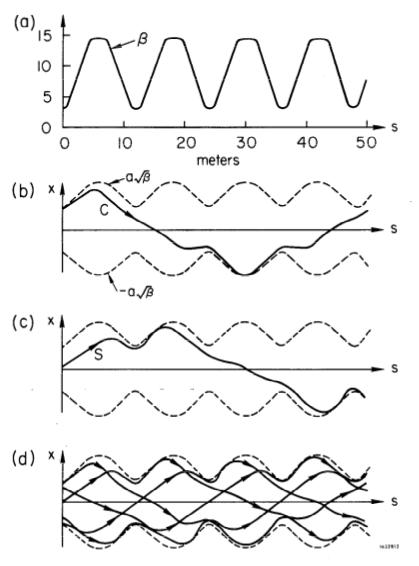
\includegraphics[width=0.7\linewidth]{./Figuras/fig12.jpeg}
	\caption{(a) Função betatron. (b) \textit{Cosine-like trajectory} para $s=0$. (c) \textit{Sine-like trajectory} para $s=0$. (d) Uma trajetória depois de várias revoluções sucessivas. Retirado de \cite{sands1970physics}.}
	\label{fig:fig12}
\end{figure}
	
Uma importante propriedade do movimento betatron é evidente na \ref{fig:fig12}(d) -- em cada coordenada, o desvio $x$ de um elétron em movimento fica sempre abaixo de um valor limitante $X(s)$, o qual é obtido colocando $cos(\varphi-\upsilon)=1$, ou seja,
	
\begin{align}
	X(s) = a\sqrt{\beta(s)}
\end{align}
	
A trajetória completa de um elétron armazenado cairá sempre dentro de um envelope definido por $\pm X(s)$. Segue que a abertura necessária para conter um elétron com uma amplitude de oscilação que varia ao redor do anel varia como $X(s)$. A relação entre a largura do envelope em duas coordenadas $s_1$ e $s_2$ é
	
\begin{align}
	\frac{X_2}{X_1} = \sqrt{\frac{\beta_2}{\beta_1}}
\end{align}
	
Para analisar a inclinação da trajetória betatron, ou seja, $x'=\frac{dx}{ds}$, considera-se a derivada da equação \eqref{eq:2.43}:
	
\begin{align}
	x' = - \frac{a}{\sqrt{\beta}}sen(\varphi-\upsilon)+\frac{\beta'}{2\beta}x\label{eq:2.52}
\end{align}
	
O primeiro termo vem da mudança de fase, e o segundo da variação de $\beta$.
	
\begin{proof}
	Seja $x(s) = a\sqrt{\beta(s)}\ cos\{\varphi(s)-\upsilon\}$. Logo, 
	\begin{align*}
      x' &= [a\sqrt{\beta}\ cos\{\varphi-\upsilon\}]'\\
         &= a[(\sqrt{\beta})'cos(\varphi-\upsilon)-\sqrt{\beta}\varphi'sen(\varphi-\upsilon)]\\
      	 &= a\left[\frac{\beta'}{2\sqrt{\beta}}cos(\varphi-\upsilon)-\sqrt{\beta}\frac{1}{\beta}sen(\varphi-\upsilon)\right]\\
      	 &= a\left[\frac{\beta'}{2\sqrt{\beta}}cos(\varphi-\upsilon)-\frac{1}{\sqrt{\beta}}sen(\varphi-\upsilon)\right]\\
      	 &= \frac{\beta'}{2\sqrt{\beta}}a\ cos(\varphi-\upsilon)-\frac{a}{\sqrt{\beta}}sen(\varphi-\upsilon)\\
      	 &= \frac{\beta'}{2\beta}a\sqrt{\beta}\ cos(\varphi-\upsilon)-\frac{a}{\sqrt{\beta}}sen(\varphi-\upsilon)\\
      	 &= -\frac{a}{\sqrt{\beta}}sen(\varphi-\upsilon)+\frac{\beta'}{2\beta}x
	\end{align*}
\end{proof}
	
Note que os zeros de $x'$ -- e, portanto, os valores de pico de $x$ -- não ocorrem em $cos(\varphi-\upsilon)=1$. Eles ocorrem em
	
\begin{align}
	tg(\varphi-\upsilon) = \frac{\beta'}{2}
\end{align}
o que significa que
\begin{align}
	cos(\varphi-\upsilon) = \left[1+\frac{\beta'^2}{4}\right]^{-\frac{1}{2}}
\end{align}
	
\begin{proof}
	Fazendo $x'=0$:
	\begin{align*}
        x'&=0\\
        -\frac{a}{\sqrt{\beta}}sen(\varphi-\upsilon)+\frac{\beta'}{2\beta}x &= 0\\
        \frac{\beta'}{2\beta}x &= \frac{a}{\sqrt{\beta}}sen(\varphi-\upsilon)\\
        \frac{\beta'}{2\beta}a\sqrt{\beta}\ cos\{\varphi-\upsilon\} &= \frac{a}{\sqrt{\beta}}sen(\varphi-\upsilon)\\
        \frac{\beta'}{2\beta}\sqrt{\beta}\sqrt{\beta} &= \frac{a}{a}\frac{sen(\varphi-\upsilon)}{cos(\varphi-\upsilon)}\\
        \frac{\beta'}{2} &= tg(\varphi-\upsilon)
	\end{align*}
	
	Pela identidade trigonométrica $1+tg^2(x) = sec^2(x)$,
	\begin{align*}
        1+tg^2(\varphi-\upsilon) &= sec^2(\varphi-\upsilon)\\
        1+\left(\frac{\beta'}{2}\right)^2 &= \left(\frac{1}{cos(\varphi-\upsilon)}\right)^2\\
        1+\frac{\beta'^2}{4} &= \frac{1}{cos^2(\varphi-\upsilon)}\\
        cos^2(\varphi-\upsilon) &= \left[1+\frac{\beta'^2}{4}\right]^{-1}\\
        cos(\varphi-\upsilon) &= \left[1+\frac{\beta'^2}{4}\right]^{-\frac{1}{2}}
	\end{align*}
	c.q.d.
\end{proof}
	
Se o pico de um ciclo particular de uma oscilação ocorrer em algum $s$, o valor de pico do desvio será
	
\begin{align}
	x_{pico} = a\sqrt{\beta}\left[1+\frac{\beta'^2}{4}\right]^{-\frac{1}{2}}
\end{align}

Veja a \autoref{fig:fig13}.

\begin{figure}[!htb]
	\centering
	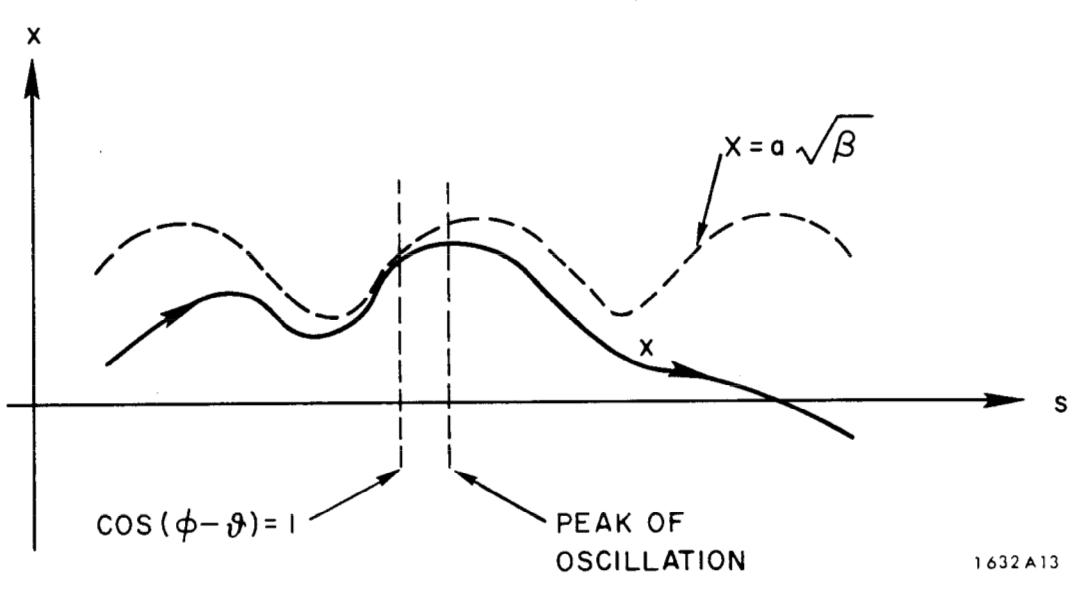
\includegraphics[width=0.8\linewidth]{./Figuras/fig13.jpeg}
	\caption{O máximo de um ciclo particular de uma oscilação betatron. Retirado de \cite{sands1970physics}.}
	\label{fig:fig13}
\end{figure}
	
Em uma oscilação harmônica clássica, a amplitude é uma invariante do movimento. Seu quadrado é proporcional à energia da oscilação, e pode ser expresso como uma função quadrática da posição e velocidade instantâneas. O invariante correspondente do oscilador pseudo-harmônico é a constante $a$, e esta pode ser obtida em termos de $x$ e $x'$ pela equação
	
\begin{align}
	a^2 = \frac{x^2}{\beta} + \beta\left[x'-\frac{\beta'}{2\beta}x\right]^2\label{eq:2.56}
\end{align}
	
\begin{proof}
	Pela equação \eqref{eq:2.43},
	\begin{align*}
        x &= a\sqrt{\beta}\ cos\{\varphi-\upsilon\}\\
        \frac{x}{a\sqrt{\beta}} &= cos(\varphi-\upsilon)\\
        \left(\frac{x}{a\sqrt{\beta}}\right)^2 &= cos^2(\varphi-\upsilon)\\
        \frac{x^2}{a^2\beta} &= cos^2(\varphi-\upsilon)
	\end{align*}
	
	Já pela equação \eqref{eq:2.52},
	\begin{align*}
        x' &= - \frac{a}{\sqrt{\beta}}sen(\varphi-\upsilon)+\frac{\beta'}{2\beta}x\\
        x' - \frac{\beta'}{2\beta}x&= - \frac{a}{\sqrt{\beta}}sen(\varphi-\upsilon)\\
        \frac{\sqrt{\beta}}{a}\left[x' - \frac{\beta'}{2\beta}x\right]&= -sen(\varphi-\upsilon)\\
        \left(\frac{\sqrt{\beta}}{a}\left[x' - \frac{\beta'}{2\beta}x\right]\right)^2&= sen^2(\varphi-\upsilon)\\
        \frac{\beta}{a^2}\left[x' - \frac{\beta'}{2\beta}x\right]^2&= sen^2(\varphi-\upsilon)
	\end{align*}
	
	Pela relação trigonométrica $sen^2(x)+cos^2(x)=1$,
	\begin{align*}
        sen^2(\varphi-\upsilon)+cos^2(\varphi-\upsilon)&=1\\
        \frac{\beta}{a^2}\left[x' - \frac{\beta'}{2\beta}x\right]^2 + \frac{x^2}{a^2\beta} &= 1\\
        \frac{1}{a^2}\left(\beta\left[x' - \frac{\beta'}{2\beta}x\right]^2 + \frac{x^2}{\beta}\right) &= 1\\
        \beta\left[x' - \frac{\beta'}{2\beta}x\right]^2 + \frac{x^2}{\beta} &= a^2
	\end{align*}
	c.q.d.
\end{proof}
	
Se os valores de $x$ e $x'$ são conhecidos em alguma coordenada, supõe-se $s_1$, então a constante $a$ pode ser obtida e todos os valores subsequentes de $x$ e $x'$ podem ser expressos por
	
\begin{align}
	x = \frac{1}{\sqrt{\beta_1}}\left[x_1^2+\left(\beta_1x'_1-\frac{x_1\beta'_1}{2}\right)^2\right]^\frac{1}{2}\sqrt{\beta}\ cos(\varphi-\upsilon)\label{eq:2.57}
\end{align}
	
\begin{proof}
	Pela equação \eqref{eq:2.56},
	\begin{align*}
        a^2 &= \frac{x^2}{\beta} + \beta\left[x'-\frac{\beta'}{2\beta}x\right]^2\\
        	&= \frac{1}{\beta}\left(x^2 + \beta^2\left[x'-\frac{\beta'}{2\beta}x\right]^2\right)\\
        	&= \frac{1}{\beta}\left(x^2 + \left[\beta x'-\frac{\beta'}{2}x\right]^2\right)\\
        \therefore a &= \left[\frac{1}{\beta}\left(x^2 + \left[\beta x'-\frac{\beta'}{2}x\right]^2\right)\right]^\frac{1}{2}\\
        	&= \frac{1}{\sqrt{\beta}}\left(x^2 + \left[\beta x'-\frac{\beta'}{2}x\right]^2\right)^\frac{1}{2}
	\end{align*}
	
	Sejam $x(s_1)=x_1$, $x'(s_1)=x'_1$ e $\beta(s_1)=\beta_1$ os valores de $x$, $x'$ e $\beta$ conhecidos no ponto $s_1$, então $a$ pode ser determinado com estes valores:
	\begin{align*}
		a = \frac{1}{\sqrt{\beta_1}}\left(x_1^2 + \left[\beta_1 x_1'-\frac{\beta_1'}{2}x_1\right]^2\right)^\frac{1}{2}
	\end{align*}
	
	Substituindo o valor de $a$ na equação \eqref{eq:2.43},
	\begin{align*}
		x &= a\sqrt{\beta}\ cos\{\varphi-\upsilon\}\\
		  &= \frac{1}{\sqrt{\beta_1}}\left[x_1^2+\left(\beta_1x'_1-\frac{x_1\beta'_1}{2}\right)^2\right]^\frac{1}{2}\sqrt{\beta}\ cos(\varphi-\upsilon)
	\end{align*}
	c.q.d.
\end{proof}
	
A constante de fase $\upsilon$ também precisa ser determinada de $x$ e $x'$, e esta pode ser obtida pela equação
	
\begin{align}
	tg(\varphi_1 - \upsilon) = -\frac{\beta_1 x'_1}{x_1}+\frac{\beta'_1}{2}
\end{align}
onde $\varphi_1 = \varphi(s_1)$.
	
\begin{proof}
	Já foi deduzido anteriormente que
	\begin{align*}
        sen(\varphi-\upsilon) &= -\frac{\sqrt{\beta}}{a}\left[x' - \frac{\beta'}{2\beta}x\right]\\
        cos(\varphi-\upsilon) &= \frac{x}{a\sqrt{\beta}}
	\end{align*}
	
	Para obter $tg(\varphi-\upsilon)$, basta
	\begin{align*}
		tg(\varphi-\upsilon) &= \frac{sen(\varphi-\upsilon)}{cos(\varphi-\upsilon)}\\
							 &= \frac{-\frac{\sqrt{\beta}}{a}\left[x' - \frac{\beta'}{2\beta}x\right]}{\frac{x}{a\sqrt{\beta}}}\\
							 &= -\frac{\sqrt{\beta}}{a}\left[x' - \frac{\beta'}{2\beta}x\right] \frac{a\sqrt{\beta}}{x}\\
							 &= \frac{\beta}{x}\left[-x' + \frac{\beta'}{2\beta}x\right]\\
							 &= -\frac{\beta x'}{x} + \frac{\beta'}{2}\\
		\therefore tg(\varphi_1-\upsilon) &= -\frac{\beta_1  x_1'}{x_1} + \frac{\beta_1'}{2}
	\end{align*}
	
	Isolando $\upsilon$, pode-se obtê-lo diretamente pela relação
	\begin{align*}
		tg(\varphi_1-\upsilon) &= -\frac{\beta_1  x_1'}{x_1} + \frac{\beta_1'}{2}\\
		cotg(tg(\varphi_1-\upsilon)) &= cotg\left(-\frac{\beta_1  x_1'}{x_1} + \frac{\beta_1'}{2}\right)\\
		\varphi_1-\upsilon &= cotg\left(-\frac{\beta_1  x_1'}{x_1} + \frac{\beta_1'}{2}\right)\\
		\upsilon &= \varphi_1 - cotg\left(-\frac{\beta_1  x_1'}{x_1} + \frac{\beta_1'}{2}\right)
	\end{align*}
\end{proof}
	
Para obter o valor máximo $X(s)$ que pode ser alcançado em qualquer $s$ em qualquer revolução subsequente, basta substituir $cos(\varphi-\upsilon)=1$ na equação \eqref{eq:2.57}:
	
\begin{align}
	X(s) = \frac{1}{\sqrt{\beta_1}}\left[x_1^2+\left(\beta_1x'_1-\frac{x_1\beta'_1}{2}\right)^2\right]^\frac{1}{2}\sqrt{\beta(s)}
\end{align}
	
Note que $X(s)$ independe de $\upsilon$.
	
Geralmente, é esperado que as amplitudes resultantes de distúrbios na trajetória serão menores quanto menor for $\beta$. De fato, pode-se considerar que $\frac{1}{\beta}$ é uma medida da "força" da focalização lateral, e que pequenos valores de $\beta$ são normalmente desejáveis. 
    \subsection{Sintonias}
	\subsection{Descrição aproximada das oscilações betatron}
Para diversos propósitos, é conveniente -- e suficiente -- aproximar o movimento betatron por uma oscilação harmônica simples. Considera-se a oscilação
\begin{align}
	x = A\ cos(s/ \lambdabar - \upsilon)\label{eq:2.66}
\end{align}
onde $\lambdabar$ é constante (o comprimento de onda reduzido). Uma oscilação completa é realizada quando $s$ avança por um comprimento de onda $2\pi \lambdabar$. É claramente conveniente pensar na oscilação pseudo-harmônica da equação \eqref{eq:2.43} como apenas uma onda senoidal com um comprimento de onda localmente variável -- se a variação de amplitude for ignorada. E, com tanto que $\beta$ não varie tão abruptamente, pode-se esperar que esta é uma aproximação razoável para o movimento real se a equação \eqref{eq:2.66} for utilizada com um $\lambdabar$ escolhido apropriadamente. Supõe-se que o número $\beta_n$ seja definido de forma a ser uma constante que dará o mesmo avanço de fase em uma revolução que a real função $\beta$. Isto é, $\beta_n$ é definido por
\begin{align}
	\int\limits_{0}^{L} \frac{ds}{\beta} = \frac{L}{\beta_n}\label{eq:2.67}
\end{align}
e é chamado de valor típico de $\beta$. Então, a oscilação
\begin{align}
	x = A\ cos(s/\beta_n + \upsilon)\label{eq:2.68}
\end{align}
irá -- com $A=a\sqrt{\beta_n}$ -- estar de acordo com a trajetória real pelo menos uma vez a cada revolução; e, em particular, irá estar, na média, em fase com a oscilação real. Na \autoref{fig:fig15} estão representadas uma das trajetórias da \autoref{fig:fig12} junto com sua aproximação obetida pela equação \eqref{eq:2.66}.

\begin{figure}[!htb]
	\centering
	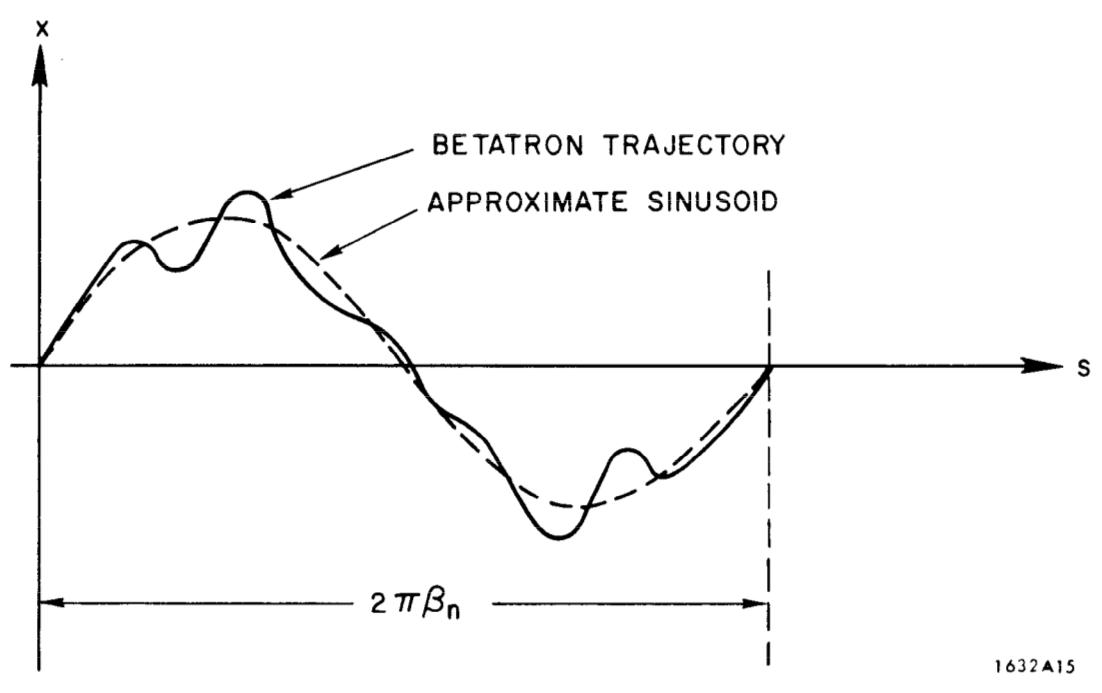
\includegraphics[width=0.7\linewidth]{./Figuras/fig15.jpeg}
	\caption{Aproximação da trajetória betatron.  ------ trajetória betatron; -- -- --  aproximação senoidal. Retirado de \cite{sands1970physics}.}
	\label{fig:fig15}
\end{figure}

É conveniente lembrar que, pela equação \eqref{eq:2.67}, $\frac{1}{\beta_n}$ é apenas a média de $\frac{1}{\beta}$ ao redor do anel:
\begin{align}
	\frac{1}{\beta_n} = \left \langle \frac{1}{\beta} \right \rangle
\end{align}

Pela definição de $\nu$ (equação \eqref{eq:2.60}), tem-se
\begin{align}
	\frac{L}{\beta_n} = 2\pi \nu
\end{align}

O raio efetivo de curvatura da órbita é dado por
\begin{align}
	R = \frac{L}{2\pi}
\end{align}
então pode-se também definir como
\begin{align}
	\beta_n = \frac{R}{\nu}
\end{align}

Note que $\beta_n$ não é igual à média de $\beta$, apesar de que também não é muito diferente se as ondulações de $\beta$ não forem muito grandes.

\begin{proof}
	Pela definição de $\nu$ e $\beta_n$ dadas respectivamente pelas equações \eqref{eq:2.60} e \eqref{eq:2.67},
	\begin{align*}
		\nu &= \frac{1}{2\pi} \int\limits_{0}^{L}\frac{ds}{\beta}\\
			&= \frac{1}{2\pi} \frac{L}{\beta_n}\\
		\therefore \frac{L}{\beta_n} &= 2\pi \nu
	\end{align*}
	
	Mas $R = L/2\pi$. Então,
	\begin{align*}
		\frac{L}{\beta_n} &= 2\pi \nu\\
		\therefore \beta_n &= \frac{L}{2\pi \nu}\\
						   &= \frac{R}{\nu}
	\end{align*}
\end{proof}

A variação de tempo da trajetória aproximada da equação \eqref{eq:2.68} é descrita como
\begin{align}
	x = A\ cos(\nu \omega_r t - \upsilon)
\end{align}
com $\omega_r = c/R$.

\begin{proof}
	Pela equação \eqref{eq:2.68}, $x = A\ cos(s/\beta_n - \upsilon)$. Agora, considerando como 0 a coordenada $s$ de referência, pela equação \eqref{eq:2.48}:
	\begin{align*}
		x &= A\ cos(s/\beta_n - \upsilon)\\
		  &= A\ cos(ct/\beta_n - \upsilon)\\
		  &= A\ cos(\nu c t/R - \upsilon)
	\end{align*}
	
	Definindo $\omega_r = c/R$, tem-se
	\begin{align*}
		x &= A\ cos(\nu \omega_r t - \upsilon)
	\end{align*}
	c.q.d.
\end{proof}

A frequência angular $\nu \omega_r$ é chamada de frequência betatron e será denominada por $\omega_\beta$. Note que, quando a trajetória aproximada é observada em um ponto fixo do anel, sua variação de tempo é indistinguível da trajetória real -- basta comparar com a equação \eqref{eq:2.64}.

A aproximação realizada nesta Seção não é adequada para vários cálculos dos efeitos do anel, mas de fato providencia a única abordagem rastreável para a análise de alguns dos efeitos coletivos que envolvem um número grande de elétrons armazenados.
	\subsection{Natureza da função beta}\label{sec:2.9}
Qual é a forma desejada de $\beta(s)$? Já foi visto que, pelo menos em alguns aspectos, pequenos valores de $\beta$ (focalização forte) são desejados -- tal que $\beta$ seja razoavelmente uniforme. Infelizmente, pequenos valores de $\beta$ só podem ser obtidos alternando o gradiente de focalização, o que tende a gerar oscilações razoavelmente grandes em $\beta$. Além disso, pequenos valores de $\beta$ implicam em grandes valores de $\nu$, o que pode gerar maiores dificuldades ao se lidar com as ressonâncias. Normalmente, $\beta$ tem um valor típico entre $1/2$ e $1/6$ do raio de curvatura $R$, não tendo, assim, oscilações muito extremas.

A função betatron é definida pela função singular, contínua a qual sua raiz quadrada satisfaz
\begin{align}
	\zeta'' = -K(s)\zeta + \frac{1}{\zeta^3}\label{eq:2.74}
\end{align}
onde $K(s)$ é a função de focalização. Tipicamente, os anéis modernos são feitos de vários segmentos nos quais a função $K(s)$ é constante, podendo ser nula, positiva ou negativa.

A imposição de que $\zeta(s)$ tem que ser periódica, juntamente com o termo não linear $1/\zeta^3$, gera uma especificação única -- incluindo a escala. A função $\zeta(s)$ é a função própria da equação \eqref{eq:2.74} e, por causa da não-linearidade, não existe uma normalização arbitrária da amplitude.

Fazendo uma análise dimensional, espera-se que $\zeta$ tenha uma dimensão $|K|^\frac{-1}{4}$, ou que $\beta$ tenha uma dimensão $|K|^\frac{-1}{2}$. (Relembrando que $1/\beta$ é como se fosse a frequência da oscilação, então é esperado que esta esteja de acordo com a raiz da constante da força restauradora). Para uma dada geometria do campo, esta lei de escala é grosseiramente verdadeira. Ela é estritamente verdadeira se a escala do comprimento da geometria de focalização é escalada em $|K|^\frac{-1}{2}$, o que geralmente é válido em campos guia bem projetados.

Em uma região de $s$ em que $K(s)$ é constante, a equação \eqref{eq:2.74} tem a forma da equação de movimento de uma partícula sob o efeito de uma força restauradora $-K\zeta$ e uma força repulsiva $1/\zeta^3$. Ou, da mesma forma, uma partícula que se move com uma energia potencial proporcional a
\begin{align}
	K\zeta^2 + \frac{1}{\zeta^2}
\end{align}
(O segundo termo é como se fosse uma barreira centrífuga!). O formato do potencial efetivo é mostrado na \autoref{fig:fig16} para os três casos de $K$.

\begin{figure}[!htb]
	\centering
	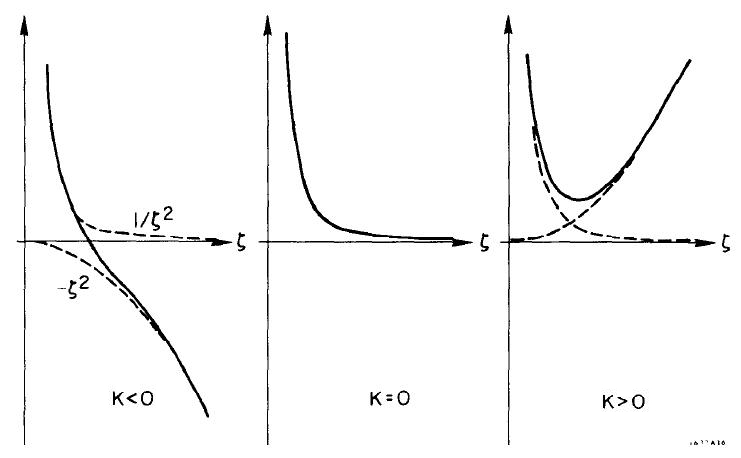
\includegraphics[width=0.9\linewidth]{./Figuras/fig16.jpeg}
	\caption{Funções potenciais efetivas para $\zeta$. Retirado de \cite{sands1970physics}.}
	\label{fig:fig16}
\end{figure}

Em qualquer região onde $K\leq 0$, a aceleração em $\zeta$ (o desvio da partícula de referência) é sempre positiva; e $\zeta$ é direcionado sempre para valores maiores -- ou, claro, dar a volta caso sua velocidade inicial seja na direção da origem de $\zeta$. Para $K$ negativo, a força direcional é, em grandes valores de $\zeta$, proporcional ao tamanho de $K$. Por outro lado, em qualquer região onde $K>0$, haverá um potencial estável e, quando $\zeta$ assume grandes valores, sempre há uma força direcionando $\zeta$ para a origem.

Também é qualitativamente aparente que possa existir soluções estáveis onde $\zeta(s)$ entra numa região onde $K<0$ movendo-se em direção à origem e muda de sentido devido à força de repulsão apenas para ser mandado na direção da origem novamente pela força de atração numa região posterior onde $K>0$. Para um K periódico como o da \autoref{fig:fig17}(a), deve-se esperar uma solução para $\zeta(s)$ como a curva representada na parte (b). A solução exibe uma importante característica geral da função $\zeta$: seu máximo ocorre em seções focalizadoras -- onde $K>0$ -- e seu mínimo ocorre em seções desfocalizadoras ou neutras -- onde $K \leq 0$.

\begin{figure}[!htb]
	\centering
	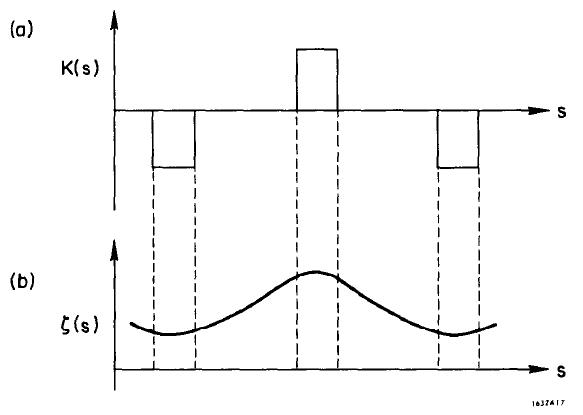
\includegraphics[width=0.7\linewidth]{./Figuras/fig17.jpeg}
	\caption{Forma da função $\zeta(s)$ com uma função de focalização $K(s)$ periódica. Retirado de \cite{sands1970physics}.}
	\label{fig:fig17}
\end{figure}

Também é evidente que para um determinado espaçamento com diferentes valores de $K$, se a magnitude de $K$ aumenta, a amplitude das oscilações irá crescer rapidamente. Menos evidente é o fato de que, conforme a escala de $K$ aumenta, chegará num ponto em que uma solução estável -- isto é, periódica -- para $\zeta(s)$ não existirá mais. Então a força de focalização (magnitude de $K$) e o espaçamento entre os elementos deve ser ajustado em conjunto, gerando a estrutura óptica do anel -- mais conhecida como \textit{lattice}, uma palavra para indicar a geometria dos segmentos.

Pode ocorrer o questionamento "Por que não apenas ter valores negativos de $K$ em todo $s$? Claramente a estabilidade de $\zeta$ é garantida". Isto não é possível pois quando $K$ é negativo em $x$, ele é automaticamente positivo em $z$, e vice-versa. Desta forma, fica claro que é necessário alternar o gradiente de focalização.

Também deve estar evidente que as oscilações de $\zeta(s)$ -- e, portanto, de $\beta(s)$ -- estarão fora de fase nas duas coordenadas transversais: $x$ e $z$. Quando $\zeta)x$ estiver em seu máximo, $\zeta_z$ estará em seu mínimo. Este comportamento é válido até nas estruturas mais complexas -- apesar de não ser totalmente verdade que $\zeta_x$ e $\zeta_z$ tem totalmente a mesma forma. 
%Na \autoref{fig:fig18} está um exemplo das funções $\zeta_x$ e $\zeta_z$.

%\begin{figure}[!htb]
%	\centering
%	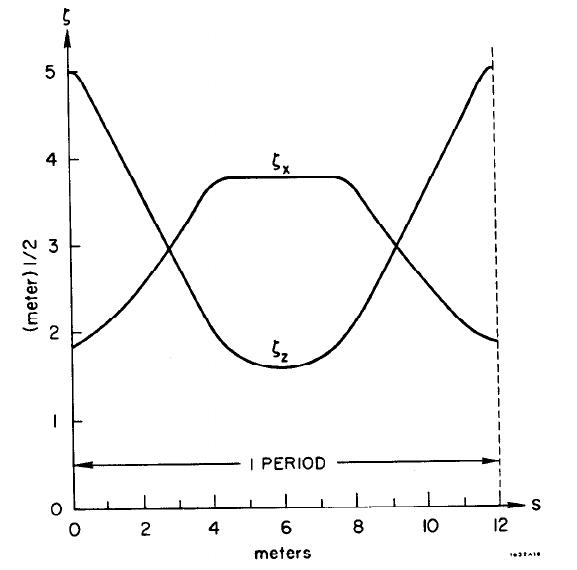
\includegraphics[width=0.7\linewidth]{./Figuras/fig18.jpeg}
%	\caption{Funções $\zeta_x$ e $\zeta_z$ de um campo guia. Retirado de \cite{sands1970physics}.}
%	\label{fig:fig18}
%\end{figure}

É intuitivo relacionar a função betatron $\beta(s)$ com a \textit{sine-like trajectory} definida na \autoref{sec:2.6}. A \textit{sine-like trajectory} $S(s,s_0)$ associada com a coordenada $s_0$ é a trajetória que começa em $s_0$ com deslocamento nulo e inclinação unitária. Esta pode ser expressa em termos da oscilação pseudo-harmônica dada pela equação \eqref{eq:2.43} substituindo $a=\sqrt{\beta(s_0)}$ e $\vartheta=\pi/2 + \varphi(s_0)$:
\begin{align}
	S(s,s_0) = \sqrt{\beta(s_0)\beta(s)}\ sen \left(\int\limits_{s_0}^{s} \frac{d\bar{s}}{\beta(\bar{s})}\right)
\end{align}
\begin{proof}
	Seja a trajetória dada pela equação \eqref{eq:2.43}:
	\begin{align*}
		x(s) = a\sqrt{\beta(s)}\ cos(\varphi(s)-\vartheta)
	\end{align*}
	com
	\begin{align*}
		\varphi(s) = \int\limits_{0}^{s} \frac{d\bar{s}}{\beta(\bar{s})}
	\end{align*}
	Substituindo $\vartheta=\pi/2 - \varphi(s_0)$:
	\begin{align*}
		x(s) &= a\sqrt{\beta(s)}\ cos(\varphi(s)-(\pi/2 + \varphi(s_0)))\\
			 &= a\sqrt{\beta(s)}\ sen(\varphi(s) - \varphi(s_0))
	\end{align*}
	Pela definição de $\varphi$,
	\begin{align*}
		x(s) &= a\sqrt{\beta(s)}\ sen\left(\int\limits_{0}^{s} \frac{d\bar{s}}{\beta(\bar{s})} - \int\limits_{0}^{s_0} \frac{d\bar{s}}{\beta(\bar{s})}\right)\\
			 &= a\sqrt{\beta(s)}\ sen\left(\int\limits_{s_0}^{s} \frac{d\bar{s}}{\beta(\bar{s})}\right)
	\end{align*}
	Substituindo $a=\sqrt{\beta(s_0)}$:
	\begin{align*}
		x(s) &= \sqrt{\beta(s_0)}\sqrt{\beta(s)}\ sen\left(\int\limits_{s_0}^{s} \frac{d\bar{s}}{\beta(\bar{s})}\right)\\
			 &= \sqrt{\beta(s_0)\beta(s)}\ sen\left(\int\limits_{s_0}^{s} \frac{d\bar{s}}{\beta(\bar{s})}\right)\\
		\therefore S(s,s_0) &= \sqrt{\beta(s_0)\beta(s)}\ sen\left(\int\limits_{s_0}^{s} \frac{d\bar{s}}{\beta(\bar{s})}\right)
	\end{align*}
	Checando,
	\begin{align*}
		S(s_0,s_0) &= \sqrt{\beta(s_0)\beta(s_0)}\ sen\left(\int\limits_{s_0}^{s_0} \frac{d\bar{s}}{\beta(\bar{s})}\right)\\
				   &= \beta(s_0)\ sen(0)\\
				   &= 0\\
		S(s,s_0)' &= \left(\sqrt{\beta(s_0)\beta(s)}\ sen\left(\int\limits_{s_0}^{s} \frac{d\bar{s}}{\beta(\bar{s})}\right)\right)'\\
				  &= \left(\sqrt{\beta(s_0)\beta(s)}\right)'\ sen\left(\int\limits_{s_0}^{s} \frac{d\bar{s}}{\beta(\bar{s})}\right) + \sqrt{\beta(s_0)\beta(s)}\ \left(sen\left(\int\limits_{s_0}^{s} \frac{d\bar{s}}{\beta(\bar{s})}\right)\right)'\\
				  &= \frac{1}{2}\frac{1}{\sqrt{\beta(s_0)\beta(s)}}(\beta(s_0)\beta(s))'\ sen\left(\int\limits_{s_0}^{s} \frac{d\bar{s}}{\beta(\bar{s})}\right) + \sqrt{\beta(s_0)\beta(s)}\ cos\left(\int\limits_{s_0}^{s} \frac{d\bar{s}}{\beta(\bar{s})}\right) \frac{1}{\beta(s)}\\
		S(s_0,s_0)' &= \frac{1}{2}\frac{1}{\sqrt{\beta(s_0)\beta(s_0)}}(\beta(s_0)\beta(s_0))'\ sen\left(\int\limits_{s_0}^{s_0} \frac{d\bar{s}}{\beta(\bar{s})}\right) + \sqrt{\beta(s_0)\beta(s_0)}\ cos\left(\int\limits_{s_0}^{s_0} \frac{d\bar{s}}{\beta(\bar{s})}\right) \frac{1}{\beta(s_0)}\\
					&= \frac{1}{2}\frac{1}{\beta(s_0)}(\beta(s_0)\beta(s_0))'\ sen(0) + \beta(s_0)\ cos(0) \frac{1}{\beta(s_0)}\\
					&= 0 + \beta(s_0)\frac{1}{\beta(s_0)}\\
					&= 1
	\end{align*}
	c.q.d.
\end{proof}

Agora, considere o que acontecerá se esta trajetória senoidal for seguida por uma volta completa -- ou seja, $s=s_0+L$. A integral fica, pela equação \eqref{eq:2.60}, apenas $2\pi\nu$. Devido à periodicidade da função betatron, $\beta(s_0+L) = \beta(s_0)$. Então,
\begin{align}
	S(s_0+L,s_0) = \beta(s_0)\ sen(2\pi\nu)
\end{align}
e, como $\nu$ independe de $s_0$, pode-se escrever também
\begin{align}
	\beta(s) = \frac{S(s+L,s)}{sen(2\pi\nu)}\label{eq:2.77}
\end{align}
Assim, a função betatron em $s$ é, a menos de uma constante, apenas o desvio após uma revolução da \textit{sine-like trajectory} começando em $s$. Veja a \autoref{fig:fig19}.

\begin{figure}[!htb]
	\centering
	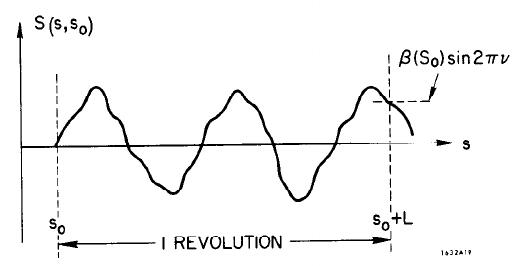
\includegraphics[width=0.8\linewidth]{./Figuras/fig19.jpeg}
	\caption{Relação entre $S(s,s_0)$ e $\beta(s_0)$. Retirado de \cite{sands1970physics}.}
	\label{fig:fig19}
\end{figure}

Pode-se obter uma outra prescrição para encontrar $\beta(s)$. Uma que precisa apenas do cálculo direto da \textit{sine-like trajectory} após uma revolução, começando em cada $s$.

O desvio obtido é proporcional a $\beta(s)$. Apenas resta determinar o fator de normalização $1/2\pi\nu$. Usando a definição de $\nu$ dada pela equação \eqref{eq:2.60}, juntamente com a equação \eqref{eq:2.77}, pode-se observar que a sintonia $\nu$ pode ser obtida como a solução da equação transcendental
\begin{align}
	\frac{2\pi\nu}{sen(2\pi\nu)} = \int\limits_{0}^{L} \frac{ds}{S(s+L,s)}
\end{align}
Então, conhecendo $S(s+L,s)$ para todo $s$, pode-se determinar $\beta(s)$ de forma única.

O cálculo de $S(s+L,s)$ pode ser efetuado por uma integração numérica da equação de movimento. Ou, para um campo guia uniforme, também pode ser obtido utilizando o método matricial descrito na \autoref{sec:2.5}. Relembrando a equação \eqref{eq:2.37}, a \textit{sine-like trajectory} de $s_0$ para $s_0+L$ é apenas o elemento da primeira linha e da primeira coluna da matriz de transferência $\boldsymbol{M}(s,s_0)$ para a máquina completa, começando em cada $s_0$.

Também pode-se mostrar que a sintonia $\nu$ pode ser obtida pelo traço da matriz para o anel todo:
\begin{align}
	cos(2\pi\nu) = \frac{1}{2} Tr \boldsymbol{M}(s+L,s) = \frac{1}{2}[C(s+L,s) + S'(s+l,s)]
\end{align}
onde $C$ é a \textit{cosine-like trajectory}. Então, se $C$ e $S'$ são calculados assim como $S$, $\nu$ pode ser determinada e a equação \eqref{eq:2.77} pode ser obtida diretamente.

Pode-se escrever a equação diferencial \eqref{eq:2.74} de $\zeta$ em termos de $\beta$:
\begin{align}
	\frac{1}{2}\beta\beta'' - \frac{1}{4}\beta'^2 + K(s)\beta^2 = 1\label{eq:2.80}
\end{align}

\begin{proof}
	Seja a equação diferencial $\zeta'' = -K(s)\zeta + \frac{1}{\zeta^3}$. Substituindo $\zeta = \sqrt{\beta}$,
	\begin{align*}
		\sqrt{\beta}'' &= -K\sqrt{\beta} + \frac{1}{\sqrt{\beta}^3}\\
		\left(\beta^\frac{1}{2}\right)'' &= -K\beta^\frac{1}{2} + \frac{1}{\beta^\frac{3}{2}}\\
		\left(\beta^\frac{1}{2}\right)''\beta^\frac{3}{2} &+ K\beta^\frac{1}{2} \beta^\frac{3}{2} = 1\\
		\left(\beta^\frac{1}{2}\right)''\beta^\frac{3}{2} &+ K\beta^2 = 1
	\end{align*}
	Derivando,
	\begin{align*}
		\left(\beta^\frac{1}{2}\right)''\beta^\frac{3}{2} + K\beta^2 &= 1\\
		\left(\frac{1}{2}\beta^\frac{-1}{2}\beta'\right)'\beta^\frac{3}{2} + K\beta^2 &= 1\\
		\left(\left(\beta^\frac{-1}{2}\right)'\beta' + \left(\beta^\frac{-1}{2}\right)\beta''\right)\frac{1}{2}\beta^\frac{3}{2} + K\beta^2 &= 1\\
		\left(\frac{-1}{2}\beta^\frac{-3}{2}\beta'\beta' + \beta^\frac{-1}{2}\beta''\right)\frac{1}{2}\beta^\frac{3}{2} + K\beta^2 &= 1\\
		\frac{-1}{4}\beta'^2 + \frac{1}{2}\beta\beta'' + K\beta^2 &= 1
	\end{align*}
	c.q.d.
\end{proof}

A partir da equação \eqref{eq:2.80}, podem-se fazer algumas observações. Primeiramente, em um trecho reto do anel (sem campo magnético), $K(s)=0$ e a solução da equação \eqref{eq:2.80} é
\begin{align}
	\beta = \beta_0\left[1+\frac{(s-s_0)^2}{\beta_0^2}\right]
\end{align}
onde $s_0$ e $\beta_0$ são constantes adequadas. Se $\beta$ tem um ponto de mínimo em um trecho reto, então $\beta_0$ e $s_0$ são os valores de $\beta$ e $s$ neste mínimo.

\begin{proof}
	A equação diferencial a ser resolvida é
	\begin{align*}
		\frac{1}{2}\beta\beta'' - \left(\frac{\beta'}{2}\right)^2
	\end{align*}
	Esta é uma equação diferencial ordinária não-linear de segunda ordem. Esta também é uma equação autônoma, ou seja, é uma equação que não contem explicitamente a variável independente -- neste caso, a coordenada $s$. Com isso, pode-se tratar a variável $\beta$ como variável independente da equação, e definir uma segunda variável $\alpha$ tal que
	\begin{align*}
		\alpha(\beta) = -\frac{\beta'}{2}
	\end{align*}
	Desta forma,
	\begin{align*}
		\beta' = -2\alpha(\beta)
		\therefore \beta'' = -2\frac{d\alpha}{d \beta}\beta' = -2\frac{d\alpha}{d \beta}(-2\alpha) = 4\alpha\frac{d\alpha}{d\beta}
	\end{align*}
	Substituindo na equação diferencial,
	\begin{align*}
		2\alpha\beta\frac{d\alpha}{d\beta} &= 1 + \alpha^2\\
		\therefore \frac{2\alpha}{1+\alpha^2}d\alpha &= \frac{1}{\beta}d\beta
	\end{align*}
	Integrando ambos os lados da equação:
	\begin{align*}
		\int \frac{2\alpha}{1+\alpha^2}d\alpha &= \int \frac{d\beta}{\beta}\\
		ln(1+\alpha^2) &= ln(\beta) + c_1\\
		ln(1+\alpha^2) - ln(\beta) &= c_1\\
		ln\left(\frac{1+\alpha^2}{\beta}\right) &= c_1
	\end{align*}
	sendo $c_1$ uma constante qualquer. Pela definição de logaritmo,
	\begin{align*}
		\frac{1+\alpha^2}{\beta} &= c_2
	\end{align*}
	sendo $c_2$ a constante dada por $e^{c_1}$. Derivando ambos os lados da expressão:
	\begin{align*}
		\frac{d}{d\beta}\left(\frac{1+\alpha^2}{\beta}\right) = 0
	\end{align*}
	Integrando esta equação diferencial de $\beta_0$ a $\beta$, tem-se
	\begin{align*}
		\frac{1+\alpha^2}{\beta} - \frac{1+\alpha_0^2}{\beta_0} = 0
	\end{align*}
	Definindo a constante $\gamma_0 = \frac{1+\alpha_0^2}{\beta_0}$, tem-se que
	\begin{align*}
		\frac{1+\alpha^2}{\beta} - \gamma_0 &= 0\\
		\frac{1+\alpha^2}{\beta} &= \gamma_0\\
		1+\alpha^2 &= \beta \gamma_0\\
		\therefore \alpha &= \sqrt{\beta\gamma_0 -1}
	\end{align*}
	Mas $\alpha = -\beta'/2$. Então,
	\begin{align*}
		-\frac{1}{2}\frac{d\beta}{ds} &= \sqrt{\beta\gamma_0 -1}\\
		\therefore -\frac{d\beta}{2\sqrt{\beta\gamma_0 -1}} &= ds
	\end{align*}
	Integrando ambos os lados da equação:
	\begin{align*}
		\int\limits_{\beta_0}^{\beta}-\frac{d\beta}{2\sqrt{\beta\gamma_0 -1}} &= \int\limits_{s_0}^{s}ds\\
		\left.\begin{matrix}
		-\frac{1}{\gamma_0}\sqrt{\beta\gamma_0-1}
		\end{matrix}\ \right|^\beta_{\beta_0} &= \left.\begin{matrix}
				s
				\end{matrix}\ \right|^s_{s_0}\\
		-\frac{1}{\gamma_0}\left(\sqrt{\beta\gamma_0-1}-\sqrt{\beta_0\gamma_0-1}\right) &= s-s_0\\
		\frac{1}{\gamma_0}\left(\sqrt{\beta_0\gamma_0-1}-\sqrt{\beta\gamma_0-1}\right) &= s-s_0\\
		\sqrt{\beta_0\gamma_0-1}-\sqrt{\beta\gamma_0-1} &= \gamma_0(s-s_0)
	\end{align*}
	Como foi definido anteriormente, $\gamma_0 = \frac{1+\alpha_0^2}{\beta_0}$. Logo,
	\begin{align*}
		\sqrt{1-\alpha_0^2-1}-\sqrt{\beta\gamma_0-1} &= \gamma_0(s-s_0)\\
		-\alpha_0-\sqrt{\beta\gamma_0-1} &= \gamma_0(s-s_0)\\
		-\sqrt{\beta\gamma_0-1} &= \alpha_0+\gamma_0(s-s_0)\\
	\end{align*}
	Elevando ambos os lados da equação ao quadrado:
	\begin{align*}
		\beta\gamma_0-1 &= [\alpha_0+\gamma_0(s-s_0)]^2\\
		\therefore \beta &= \frac{1}{\gamma_0}[1+(\alpha_0+\gamma_0(s-s_0))^2]
	\end{align*}
	No ponto de mínimo da função, $\beta'=0$ e, portanto, $\alpha=0$. Substituindo na solução obtida:
	\begin{align*}
		\beta &= \beta_0\left[1+\frac{1}{\beta_0^2}(s-s_0)^2\right]
	\end{align*}
	c.q.d.
\end{proof}

A forma desta solução é ilustrada na \autoref{fig:fig20}. Note que o coeficiente do termo quadrático é o inverso do valor de $\beta$ no seu ponto mínimo -- quanto menor for $\beta_0$. mais rápido é o aumento de $\beta$ com o aumento da distância do ponto de mínimo.


Finalmente, observe que, em um segmento que $K$ é grande e $\beta'$ pequeno, a equação \eqref{eq:2.80} pode ser aproximada por
\begin{align}
	\beta'' = -2K\beta
\end{align}
Assim, $\beta$ é uma senoide ou uma exponencial dependendo do sinal de $K$.

\begin{figure}[!htb]
	\centering
	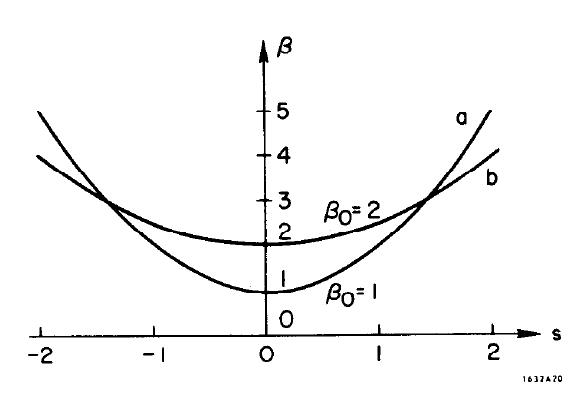
\includegraphics[width=0.7\linewidth]{./Figuras/fig20.jpeg}
	\caption{Variação de $\beta$ próximo do mínimo o qual ocorre em um longo trecho reto (sem campo magnético). Retirado de \cite{sands1970physics}.}
	\label{fig:fig20}
\end{figure}
	\subsection{Perturbação de órbita fechada}\label{sec:2.10}
Até o presente momento, foram consideradas as trajetórias de um elétron em um campo guia pré-definido. Agora, deseja-se considerar a seguinte pergunta: suponha que toda a análise sobre a trajetória dos elétrons foi feita acerca de um campo guia pré-definido; como as trajetórias irão variar se existirem pequenos erros no campo com relação ao campo pré-definido? Considerando a aproximação linear realizada até aqui, o campo guia pré-definido -- ou nominal -- é especificado pelo seu valor na órbita ideal e sua derivada radial. Além disso, assume-se que o campo na órbita ideal é vertical em todo o anel. E se o campo magnético vertical na órbita ideal diferir do seu valor nominal, ou se existirem pequenas componentes horizontais de campo, as acelerações laterais serão diferentes das especificações necessárias para manter o elétron na órbita ideal. Os desvios do campo na órbita ideal serão chamam-se erros de campo, enquanto mudanças no campo que fazem com que as funções de focalização $K_x$ e $K_z$ tenham valores diferentes de seus valores nominais chamam-se erros de gradiente.

Quando existem erros de campo, a órbita ideal deixa de ser uma trajetória possível. Se os erros são pequenos, no entanto, irá existir uma outra órbita fechada a qual é uma trajetória possível a um elétron com energia nominal. Esta trajetória é chamada de órbita fechada. Esta trajetória irá executar as oscilações betatron relativas à órbita fechada. E a forma das oscilações betatron será determinada pelas novas funções de focalização. Isto é, mantendo $x$ como sendo a representação do desvio radial da órbita ideal, este pode ser descrito como
\begin{align}
	x = x_c + x_\beta\label{eq:2.83}
\end{align}
onde $x_c$ é o desvio da órbita fechada com relação à órbita ideal, e $x_\beta$ é a oscilação betatron com relação à órbita fechada.

Se os desvios da órbita fechada com relação à órbita ideal são pequenos, então as oscilações betatron são as mesmas, tanto com relação à órbita ideal quanto com relação à órbita fechada -- assumindo uma variação linear do campo. Desta forma, pode-se considerar separadamente a distorção da órbita fechada causada pelos erros de campo e os distúrbios nas oscilações betatron causados pelos erros de gradiente. Seguindo esta ideia, a equação \eqref{eq:2.83} pode ser interpretada como uma superposição da distorção da órbita fechada $x_c$ e a oscilação betatron $x_\beta$ calculada com relação à órbita ideal pelos métodos já estudados.

Analisando primeiramente os erros de campo. Suponha que os efeitos dos erros de campo existentes apenas em pequenos intervalos $\Delta s$ analisados a partir de $s=0$ comecem a ser considerados. Passando por $\Delta s$, o desvio $x$ não se altera, mas a inclinação $x'$ é alterada pela quantidade
\begin{align}
	\Delta x' = -\frac{ec\ \delta B}{E_0}\Delta s
\end{align}
onde $\delta B$ é o desvio do campo magnético com relação ao seu valor nominal.

\begin{proof}
	Fazendo um raciocínio bem informal, já foi visto que
	\begin{align*}
		d\theta = -\frac{ecB}{E}d\ell
	\end{align*}
	Considerando $d\ell$ pequeno, pode-se aproximar que $dx = d\ell$. Assim,
	\begin{align*}
		d\theta = -\frac{ecB}{E}ds
	\end{align*}
	Analisando apenas para uma pequena modificação no campo magnético, para um elétron com energia nominal:
	\begin{align*}
		d\theta = -\frac{ec\ \delta B}{E_0}ds
	\end{align*}
	Analisando para um intervalo $\Delta s$,
	\begin{align*}
		\Delta\theta = -\frac{ecB}{E}\Delta s
	\end{align*}
	Mas $\Delta \theta$ é a variação da inclinação $x'$, logo
	\begin{align*}
		\Delta x' = -\frac{ecB}{E}\Delta s
	\end{align*}
	Uma formulação mais rigorosa pode ser obtida analisando a força de Lorentz.
\end{proof}

Para o movimento vertical, pode-se obter uma equação da mesma forma se $\delta B$ for definido como o campo radial total na órbita ideal (com uma escolha adequada de sinal). Mantendo a definição da equação \eqref{eq:2.3}, tem-se que $-ec\ \delta B/E_0 = -\delta G$, considerando as coordenadas transversais $x$ e $z$. Para facilitar a análise, será considerada apenas uma coordenada $x$ genérica, lembrando que os resultados obtidos valem tanto para o movimento radial quanto para o vertical. Desta forma, pode-se reescrever a equação anterior como sendo
\begin{align}
	\Delta x' = -\delta G \Delta s\label{eq:2.84}
\end{align}

O erro de campo adiciona à relação $x'' = \Delta x'/ \Delta s$ o termo $-\delta G$; e é, portanto, equivalente a adicionar uma força direcional $\delta G(s)$ à equação de movimento. Pode-se obter a equação completa para $x_c$ adicionando esta nova força à equação diferencial de costume, equação \eqref{eq:2.31}:
\begin{align}
	x'' = -K(s)x - \delta G(s)\label{eq:2.85}
\end{align}
O desvio $x_c$ da órbita fechada é a solução desta equação singular.

Pode-se fazer uma estimativa do efeito de um erro de campo localizado em $s=0$ usando a forma harmônica aproximada do movimento betatron descrita na \autoref{sec:2.8}. Pense em um elétron viajando ao longo da órbita ideal -- de forma que a inclinação $x'$ seja nula. Quando este elétron chegar em $s=0$, sua inclinação será subitamente alterada para $\Delta x'$. Veja a \autoref{fig:fig21}. 

\begin{figure}[!htb]
	\centering
	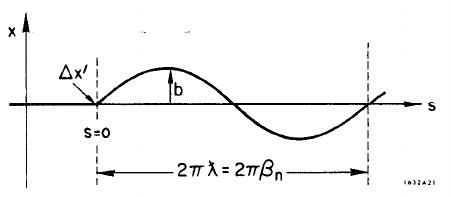
\includegraphics[width=0.7\linewidth]{./Figuras/fig21.jpeg}
	\caption{Efeito de um erro de campo localizado. Retirado de \cite{sands1970physics}.}
	\label{fig:fig21}
\end{figure}
Depois de $s=0$ não há erro de campo (para uma volta completa) então o elétron começa a oscilar em torno da órbita ideal com amplitude
\begin{align}
	b = \lambdabar \Delta x' = \beta_n \Delta x' = -\beta_n\ \delta G \Delta s\label{eq:2.86}
\end{align}
É esperado que o desvio da órbita fechada $x_c$ seja da mesma ordem de grandeza.

\begin{proof}
	Matematicamente, uma senoide com fase nula é descrita por
	\begin{align*}
		x(s) = b\ sen\left(\frac{2\pi s}{\lambda}\right)
	\end{align*}
	onde $b$ é a amplitude da oscilação e $\lambda$ é seu comprimento de onda. Desta forma,
	\begin{align*}
		x'(s) &= \frac{2\pi}{\lambda}b\ cos\left(\frac{2\pi s}{\lambda}\right)\\
		\therefore x'(0) & = \frac{2\pi}{\lambda}b\\
		\therefore b &= \frac{\lambda}{2\pi}x'(0)
	\end{align*}
	Já foi visto na \autoref{sec:2.8} que $\lambdabar = \lambda/2\pi$, então
	\begin{align*}
		b &= \lambdabar x'(0)
	\end{align*}
	Mas, considerando a análise que está sendo feita, $x'(0) = \Delta x'$. Logo,
	\begin{align*}
		b &= \lambdabar \Delta x'
	\end{align*}
	Também na \autoref{sec:2.8} mostrou-se que $\lambdabar = \beta_n$, então
	\begin{align*}
		b &= \beta_n \Delta x'\\
		  &= -\beta_n\ \delta G \Delta s
	\end{align*}
	c.q.d.
\end{proof}

Para fazer o cálculo de $x_c$ de forma apropriada, deve-se utilizar a oscilação pseudo-harmônica correta, e lembrar também que a órbita fechada é definida como a trajetória particular que fecha nela mesma após uma revolução. Em outras palavras, $x_c$ deve ser uma função singular em cada coordenada física $s$, ou seja, $x_c(s+L) = x_c(s)$. Em particular,
\begin{align}
	x_c(L) = x_c(0)\label{eq:2.87}
\end{align}
e, pela equação \eqref{eq:2.84},
\begin{align}
	x'_c(L) - \delta G \Delta s = x'_c(0)\label{eq:2.88}
\end{align}
Mas entre $s=0$ e $s=L$ não existem erros de campo, então $x_c$ é apenas uma oscilação livre entorno da órbita ideal. Veja a \autoref{fig:fig22}. Isto é, $x_c$ deve ser dado pela equação \eqref{eq:2.43}:
\begin{align}
	x_c(s) = a\sqrt{\beta(s)}cos(\varphi - \vartheta),\ s \neq 0,\label{eq:2.89}
\end{align}
com constantes arbitrárias $a$ e $\vartheta$ escolhidas de tal maneira que as equações \eqref{eq:2.87} e \eqref{eq:2.88} sejam satisfeitas.

\begin{figure}[!htb]
	\centering
	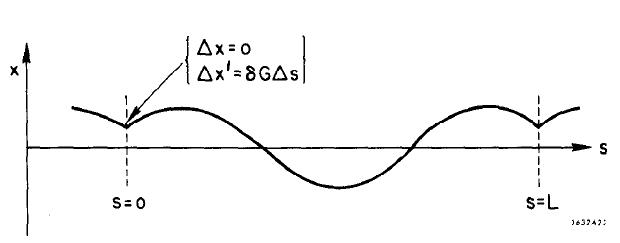
\includegraphics[width=0.7\linewidth]{./Figuras/fig22.jpeg}
	\caption{Órbita fechada para um erro de campo em $s=0$. Retirado de \cite{sands1970physics}.}
	\label{fig:fig22}
\end{figure}

Utilizando a equação \eqref{eq:2.52} para $x'_c(s)$ -- em todo o anel exceto em $s=0$ -- pode-se verificar que os valores apropriados para $a$ e $\vartheta$ são
\begin{align}
	a &= -\frac{\delta G\ \Delta s\ \sqrt{\beta(0)}}{2 sen(\pi \nu)}\\
	\vartheta &= \pi \nu
\end{align}

\begin{proof}
	Seja $x_c(L)$ dado pela equação \eqref{eq:2.89}:
	\begin{align*}
		x_c(L) = a\sqrt{\beta(L)}\ cos(\varphi(L)-\vartheta)
	\end{align*}
	Pela definição de $\varphi(s)$ e $\nu$,
	\begin{align*}
		x_c(L) = a\sqrt{\beta(L)}\ cos(2\pi\nu-\vartheta)
	\end{align*}
	Mas, a condição da equação \eqref{eq:2.87} deve ser satisfeita. Logo,
	\begin{align*}
		x_c(L) &= x_c(0)\\
		a\sqrt{\beta(L)}\ cos(2\pi\nu-\vartheta) &= a\sqrt{\beta(0)}\ cos(\varphi(0)-\vartheta)
	\end{align*}
	Novamente, pela definição de $\varphi(s)$,
	\begin{align*}
		a\sqrt{\beta(L)}\ cos(2\pi\nu-\vartheta) &= a\sqrt{\beta(0)}\ cos(-\vartheta)
	\end{align*}
	Pela periodicidade da função $\beta$,
	\begin{align*}
		a\sqrt{\beta(0)}\ cos(2\pi\nu-\vartheta) &= a\sqrt{\beta(0)}\ cos(-\vartheta)\\
		cos(2\pi\nu-\vartheta) &= cos(-\vartheta)
	\end{align*}
	Como cosseno é uma função par,
	\begin{align*}
		cos(2\pi\nu-\vartheta) &= cos(\vartheta)\\
		\therefore 2\pi\nu - \vartheta &= \vartheta\\
		\therefore \vartheta &= \pi\nu
	\end{align*}
	Agora, seja $x'_c(L)$ dado pela equação \eqref{eq:2.52}:
	\begin{align*}
		x'_c(L) &= -\frac{a}{\beta(L)}\ sen(\varphi(L)-\vartheta) + \frac{\beta'(L)}{2\beta(L)}x_c(L)\\
				&= -\frac{a}{\beta(L)}\ sen(2\pi\nu-\pi\nu) + \frac{\beta'(L)}{2\beta(L)}x_c(L)\\
				&= -\frac{a}{\beta(L)}\ sen(\pi\nu) + \frac{\beta'(L)}{2\beta(L)}x_c(L)
	\end{align*}
	A condição da equação \eqref{eq:2.88} impõe que
	\begin{align*}
		x'_c(L) - \delta G\ \Delta s &= x'_c(0)\\
		-\frac{a}{\beta(L)}\ sen(\pi\nu) + \frac{\beta'(L)}{2\beta(L)}x_c(L) - \delta G\ \Delta s &= -\frac{a}{\beta(0)}\ sen(\varphi(0)-\pi\nu) + \frac{\beta'(0)}{2\beta(0)}x_c(0)\\
		-\frac{a}{\beta(L)}\ sen(\pi\nu) + \frac{\beta'(L)}{2\beta(L)}x_c(L) - \delta G\ \Delta s &= -\frac{a}{\beta(0)}\ sen(0-\pi\nu) + \frac{\beta'(0)}{2\beta(0)}x_c(0)\\
		-\frac{a}{\beta(L)}\ sen(\pi\nu) + \frac{\beta'(L)}{2\beta(L)}x_c(L) - \delta G\ \Delta s &= -\frac{a}{\beta(0)}\ sen(-\pi\nu) + \frac{\beta'(0)}{2\beta(0)}x_c(0)
	\end{align*}
	Pela periodicidade da função $\beta(s)$ e a restrição imposta pela equação \eqref{eq:2.87},
	\begin{align*}
		-\frac{a}{\beta(0)}\ sen(\pi\nu) + \frac{\beta'(0)}{2\beta(0)}x_c(0) - \delta G\ \Delta s &= -\frac{a}{\beta(0)}\ sen(-\pi\nu) + \frac{\beta'(0)}{2\beta(0)}x_c(0)\\
		\therefore -\frac{a}{\beta(0)}\ sen(\pi\nu) - \delta G\ \Delta s &= -\frac{a}{\beta(0)}\ sen(-\pi\nu)
	\end{align*}
	Como seno é uma função ímpar,
	\begin{align*}
		-\frac{a}{\beta(0)}\ sen(\pi\nu) - \delta G\ \Delta s &= \frac{a}{\beta(0)}\ sen(\pi\nu)\\
		\therefore \frac{a}{\beta(0)}\ 2sen(\pi\nu) &= -\delta G\ \Delta s\\
		\therefore a = -\frac{\delta G\ \Delta s\ \sqrt{\beta(0)}}{2 sen(\pi \nu)}
	\end{align*}
	c.q.d.
\end{proof}

O desvio da órbita fechada é, portanto,
\begin{align}
	x_c(s) = -\frac{\delta G\ \Delta s\ \sqrt{\beta(0)}}{2 sen(\pi \nu)}\ \sqrt{\beta(s)}\ cos(\varphi(s)-\pi\nu)\label{eq:2.92}
\end{align}

A forma do invariante $a$ da amplitude mostra duas características interessantes da órbita fechada. Primeiramente, note que o desvio da órbita fechada é em todo o anel proporcional à "força" $\ \delta G \Delta s$ do erro de campo, e à raiz de $\beta(0)$, a magnitude da função betatron no local da perturbação. Agora entende-se porque $\beta(s)$ -- ou mais precisamente $\zeta(s) = \sqrt{\beta(s)}$ -- é uma medida da "sensibilidade" à distúrbios.

Segundo, note que o denominador de $a$ vai para zero, e $x_c$ se torna, portanto, muito grande sempre que a sintonia $\nu$ se aproxima de um inteiro. É este comportamento o qual foi referido anteriormente como "ressonância inteira", a qual deve ser evitada escolhendo o ponto de operação $(\nu_x,\nu_z)$ longe de números inteiros.

Note que o desvio da órbita fechada no local do erro de campo tem uma forma particularmente simples. Basta apenas analisar a equação \eqref{eq:2.92} considerando $s=0$, ou generalizar para um erro de campo localizado em uma coordenada arbitrária $s_1$, obtendo
\begin{align}
	x_c(s_1) = -\delta G\ \Delta s \frac{\beta(s_1)}{2 tg(\pi\nu)}
\end{align}
Agora o desvio é proporcional à primeira potência de $\beta$, mas a dependência da ressonância de $\nu$ ainda é evidente no termo da tangente. Note também que, exceto pelo denominador ressonante, o resultado confere com a estimativa dada pela equação \eqref{eq:2.86}.

A equação \eqref{eq:2.92} também pode ser generalizada para uma órbita fechada com erros de campo que seguem uma distribuição arbitrária ao longo do anel. Em cada coordenada $s$, os desvios da órbita fechada causados por erros em todas as outras coordenadas irão se somar. Para um erro em $\bar{s}$, deve-se substituir $s=0$ por $\bar{s}$ na equação \eqref{eq:2.92} -- e, ao mesmo tempo, substituir $\varphi(s)$ por $|\varphi(s) - \varphi\bar{s}|$. Assim, somando sobre todos os $\Delta \bar{s}$, tem-se 
\begin{align}
	x_c(s) = -\frac{\sqrt{\beta(s)}}{2sen(\pi\nu)}\int\limits_{0}^{L}\delta G(\bar{s})\sqrt{\beta(\bar{s})}cos(|\varphi(s)-\varphi(\bar{s})|-\pi\nu)d\bar{s}\label{eq:2.94}
\end{align}
Se o desvio de campo $\delta G(s)$ é conhecido, esta equação dará a forma da órbita fechada (considerando os valores nominais de $\beta(s)$ e $\nu$).

Se os desvios de campo são verdadeiros "erros" com uma distribuição estatística desconhecida, uma análise estatística mais complexa deve ser feita para chegar na estimativa estatística de $x_c$.

Como foi dito anteriormente, o desvio total da órbita ideal é dado pela soma de $x_c$ e a oscilação betatron. Na próxima análise, $x_c$ será ignorado -- lembrando sempre que este precisa ser adicionado quando pretende-se analisar o desvio total da trajetória com relação à órbita ideal.
	\subsection{Erros de gradiente de campo}
Agora, pode-se analisar os efeitos dos erros de gradiente nas oscilações betatron em torno da órbita ideal. estes "erros" são relativos aos desvios da função de focalização $K(s)$ do seu valor nominal em cada coordenada $s$. Pode-se escrever
\begin{align*}
	K(s)_{atual} = K(s)_{nominal} + k(s)
\end{align*}
onde assume-se que $k(s)$ é pequeno. O efeito do desvio $k(s)$ será mudar a função betatron do seu valor nominal $\beta(s)$ para um novo valor $\beta(s)+\Delta \beta(s)$. Desta forma, a sintonia também será alterada do seu valor nominal $\nu$ para um novo valor $\nu + \Delta \nu$. Geralmente, a mudança de sintonia $\Delta \nu$ é mais preocupante, uma vez que esta pequena mudança pode fazer com que o ponto de operação da máquina entra em uma ressonância.

Suponha que existe um erro de gradiente $k$ apenas em um pequeno intervalo $\Delta s$ em $s=0$. Então um elétron que passa em $s=0$ irá receber um \textit{kick} angular extra $\Delta x'$ proporcional ao seu desvio $x$. Isto é,
\begin{align}
	\Delta x' = -k\ \Delta s\ x\label{eq:2.96}
\end{align}

\begin{proof}
	Fazendo um raciocínio bem informal, sabe-se que a equação diferencial que descreve o movimento do elétron é
	\begin{align*}
		x'' = -K(s)x
	\end{align*}
	A derivada nada mais é que a variação de $x'$ em um intervalo $s$ pequeno, então $x'' = \Delta x'/\Delta s$. Logo,
	\begin{align*}
		\frac{\Delta x'}{\Delta s} &= -K(s)x\\
		\Delta x' &= -K(s)x \Delta s
	\end{align*}
	Analisando apenas a variação de $x'$ causada pela variação $k(s)$ da função de focalização, tem-se
	\begin{align*}
		\Delta x' &= -k\ \Delta s\ x
	\end{align*}
\end{proof}

Aproximando novamente a função betatron por uma simples oscilação harmônica, o que aconteceria se um elétron chegasse em $s=0$ no pico da oscilação? o movimento seria como a curva representada na \autoref{fig:fig23}.

\begin{figure}[!htb]
	\centering
	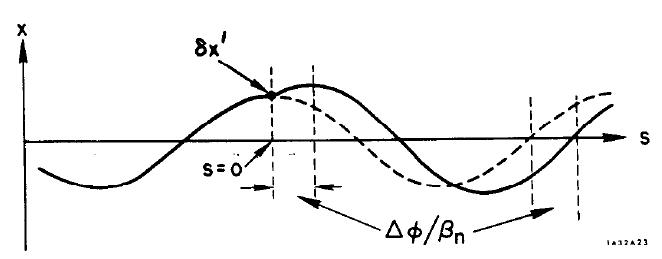
\includegraphics[width=0.7\linewidth]{./Figuras/fig23.jpeg}
	\caption{Efeito do gradiente de erro em $s=0$. Retirado de \cite{sands1970physics}.}
	\label{fig:fig23}
\end{figure}

Antes de chegar em $s=0$. o desvio era dado por
\begin{align}
	x = b\ cos(s/\beta_n)
\end{align}
e, depois de $s=0$, seguirá uma trajetória
\begin{align}
	x = (b+\Delta b)cos(s/\beta_n + \Delta \varphi)
\end{align}
onde
\begin{align}
	-\frac{b+\Delta b}{\beta_n}\ sen(\Delta \varphi) = \Delta x'
\end{align}

\begin{proof}
	Seja a solução da equação diferencial $x'' = -Kx$ dada por $x = a\ cos(\varphi-\vartheta)$. Para $K(s) = K(s)_{nominal}$ já foi visto que existe a solução aproximada $x = b\ cos(s/\beta_n)$. Quando o elétron passa em $s=0$, a equação diferencial deixa de ser $x'' = -K(s)_{nominal}\ x$ e passa a ser $x'' = -K(s)_{atual}\ x$ onde $K(s)_{atual} = K(s)_{nominal} + k(s)$. Logo, a equação diferencial é dada por $x'' = -(K(s)_{nominal} + k(s))x$. Esta mudança na função de focalização $K(s)$ acarretará numa mudança $\Delta \beta$ no valor da função betatron. Como tanto a amplitude quanto a fase de oscilação dependem de $\beta(s)$, ambas sofreram alterações, as quais foram denominadas $\Delta b$ e $\Delta \varphi$, respectivamente. Sendo assim, a solução desta nova equação diferencial pode ser escrita como
	\begin{align*}
		x = (b+\Delta b)\ cos(s/\beta_n + \Delta \varphi)
	\end{align*}
	Nota-se que o termo $\Delta \varphi$ não está multiplicado pela variável $s$ como o termo $1/\beta_n$. Isto porque a alteração na fase da oscilação ocorre somente no ponto $s=0$, diferentemente do avanço de fase descrito pelo termo $s/\beta_n$.
	
	Agora, derivando a expressão $x = b\ cos(s/\beta_n)$, tem-se
	\begin{align*}
		x' &= -b\ sen(s/\beta_n)\\
		\therefore x'(0) &= 0 = x'_i
	\end{align*}
	Derivando a expressão $x = (b+\Delta b)\ cos(s/\beta_n + \Delta \varphi)$, tem-se
	\begin{align*}
		x' = -\frac{b+\Delta b}{\beta_n}\ sen(s/\beta_n + \Delta \varphi)\\
		x'(0) = -\frac{b+\Delta b}{\beta_n}\ sen(\Delta \varphi) = x'_f
	\end{align*}
	Desta forma, a variação $\Delta x'$ da inclinação do movimento no ponto $s=0$ é
	\begin{align*}
		\Delta x' &= x'_f - x'_i\\
				  &= -\frac{b+\Delta b}{\beta_n}\ sen(\Delta \varphi) - 0\\
				  & = -\frac{b+\Delta b}{\beta_n}\ sen(\Delta \varphi)
	\end{align*}
	c.q.d.
\end{proof}

Para pequenos valores de $\Delta x'$, $\Delta \varphi$ é pequeno (ou seja, pode-se aproximar $sen(\varphi) = \varphi$) e $\Delta b$ é muito menor que $b$. Logo,
\begin{align}
	\Delta \varphi \approx -\frac{\beta_n\ \Delta x'}{b}
\end{align}
Utilizando a equação \eqref{eq:2.96} -- e lembrando que em $s=0$ o deslocamento é $b$ -- tem-se que
\begin{align*}
	\Delta \varphi = \beta_n\ k\ \Delta s
\end{align*}
O efeito do erro de gradiente é basicamente alterar a fase de oscilação por $\Delta \varphi$. Agora, lembre-se que $2\pi\nu$ é o avanço de fase total em uma revolução; então, grosseiramente falando, o erro de gradiente acarreta em
\begin{align}
	\Delta \nu \approx - \frac{\Delta \varphi}{2\pi} = -\frac{\beta_n\ k\ \Delta s}{2\pi}
\end{align}
O sinal negativo vem do fato de que o avanço total de fase é reduzido.

Este resultado é, na verdade, até duas vezes maior do que o normal. O motivo é que o cálculo de $\Delta \varphi$ foi feito no caso especial do elétron chegando em $s=0$ no pico da oscilação. Se o elétron chegar em $s=0$ com uma fase $\varphi_0$, a mudança de fase $\delta \varphi$ é reduzida por um fator $cos^2(\varphi_0)$. Como $\varphi_0$ assume vários valores ao longo de sucessivas voltas, pode-se esperar que a média de $\Delta \varphi$ seja reduzida pela média de $cos^2(\varphi_0)$, que é apenas $1/2$. Com esta correção, a estimativa de $\Delta \nu$ fica
\begin{align}
	\Delta \nu = -\frac{1}{4\pi}\beta(s)\ k\ \Delta s
\end{align}

Note que a mudança da sintonia é proporcional ao erro de gradiente em qualquer ponto e ao valor de $\beta$ neste ponto. Novamente, pode-se observar que a função $\beta$ é um indicador da sensibilidade do anel a imperfeições.

Se existe um erro de gradiente $k(s)$ distribuído ao longo do anel, a alteração total da sintonia é
\begin{align}
	\Delta \nu = -\frac{1}{4\pi} \int\limits_{0}^{L}\beta(s)k(s)ds\label{eq:2.104}
\end{align}

Foi dito anteriormente que é esperado que $\Delta \nu$ seja da dimensão de $\nu$, então grandes valores de $\nu$ devem ser evitados. Para checar este fato, lembre (da \autoref{sec:2.10}) que $\beta$ é esperado para ser escalado como $|K|^{-1/2}$. Sendo assim, $\nu$ deve ter a mesma dimensão que $|K|^{1/2}$. Da equação \eqref{eq:2.104}, $\Delta \nu$ deve ser da magnitude de $k\beta$, então $\Delta \nu/\nu$ deve ser da mesma dimensão que $k/K$. Para um dado tamanho relativo do erro de gradiente, a alteração da sintonia $\Delta \nu$ é proporcional a $\nu$. Mas o espaço entre as ressonâncias é independente de $\nu$, então grandes valores de $\nu$ implicam em uma máquina mais delicada.

Uma mudança em $\nu$ implica que deve ter ocorrido uma mudança em $\beta$, a qual ainda não ficou muito evidente nos cálculos realizados. Pode-se mostrar que
\begin{align}
	\Delta \beta(s) = \frac{\beta(s)}{2\ sen(2\pi\nu)}\int\limits_{0}^{L}k(\bar{s})\ \beta(\bar{s})\ cos\ 2\{|\varphi(s)-\varphi(\bar{s})|-\pi\nu\}d\bar{s}\label{eq:2.105}
\end{align}
onde, como já é conhecido,
\begin{align}
	\varphi(s) = \int\limits_{0}^{s}\frac{d\bar{s}}{\beta(\bar{s})}
\end{align}

Pode-se comparar este resultado com o que foi obtido na equação \eqref{eq:2.94} para as distorções de órbita fechada. A forma é similar, mas com duas diferenças importantes. Primeiro, enquanto $\beta^{1/2}$ aparece na integral para os desvios da órbita fechada, $\beta$ aparece na integral para $\Delta \beta$. Segundo, note que o argumento do termo senoidal no denominador é $2\pi\nu$ ao invés de $\pi\nu$. A "explosão" ressonante ocorre tanto nos valores inteiros quanto nos meio inteiros de $\nu$. O erro de gradiente introduz um novo grupo de ressonâncias no diagrama de operação de $\nu_x$ po $\nu_z$, as quais devem ser evitadas em um anel de armazenamento em operação.

A mudança de sintonia $\Delta \nu$ vem, claro, da mudança na função betatron. Da definição de $\nu$, pode-se escrever
\begin{align}
	2\pi\nu = \int\limits_{0}^{L}\frac{\Delta \beta(s)}{\beta^2(s)}ds
\end{align}
Uma integração em $s$ de $\Delta \beta(s)/\beta^2(s)$ utilizando a equação \eqref{eq:2.105} chega no mesmo resultado para $\Delta \nu$ obtido na equação \eqref{eq:2.104}.

Neste ponto, pode-se esperar um certo questionamento: por que $\Delta \beta$ tem uma explosão ressonante em valores meio inteiros de $\nu$ e a mudança de sintonia $\Delta \nu$ não? A razão para este fato é que a expressão derivada para $\Delta \nu$ é válida apenas para pequenas variações de $\beta$, o que não acontece em ressonâncias, nas quais $\beta$ diverge. Um cálculo mais preciso deve ser feito, mantendo os efeitos de segunda ordem causados pela perturbação $k$, para encontrar $\Delta \nu$ -- e, de fato, o próprio $\Delta \beta$ -- próximo a uma ressonância.
	\pagebreak
	
\section{Oscilações em Energia}
	\subsection{Órbitas fechadas}
Nas discussões anteriores, foram analisadas trajetórias em anéis de armazenamento de elétrons com energia nominal $E_0$ --  a qual é a energia projetada para uma dada configuração ótica. No entanto, nem todos os elétrons armazenados possuem esta energia ideal. No geral, a energia $E$ de um elétron armazenado irá diferir da energia nominal, oscilando em torno desta. Estas oscilações de energia -- comumente chamadas de ''oscilações síncronas'' -- são o objeto de estudo desta seção.

Primeiramente, é necessário entender o movimento destes elétrons cuja energia difere de uma pequena quantidade $\epsilon$ da energia nominal. Mantendo a condição da \autoref{sec:3.2} de que a órbita ideal se encontra no plano horizontal, desvios de energia irão, para termos de primeira ordem, afetar apenas o movimento radial. O desvio vertical irá ser descrito apenas pelas oscilações betatron descritas na \autoref{part2}, e não serão consideradas nesta análise. Da \autoref{sec:2.6}, foi conveniente deixar que o símbolo $x$ representasse tanto $x_\beta$ quando $z_\beta$, os desvios laterais associados às oscilações betatron. A partir de agora, $x$ volta a representar o desvio horizontal total da trajetória com relação à órbita ideal.

Foi mostrado na \autoref{sec:2.5} que em um campo guia ideal o movimento radial de um elétron com um desvio de energia $\epsilon$ pode ser descrito pela soma de duas partes:
\begin{align}
	x = x_\beta + x_\epsilon
\end{align}
onde $x_\beta$ é o desvio causado pelas oscilações betatron e $x_\epsilon$ o desvio que depende apenas da energia do elétron. Acrescentando os resultados obtidos na \autoref{sec:2.11}, deve-se incluir o termo referente à distorção da órbita fechada devido às imperfeições magnéticas e escrever
\begin{align}
	x = x_\beta + x_\epsilon + x_c
\end{align}
Devido ao fato de que estes termos contribuem de forma linear -- assumindo um campo guia linear, pequenos desvios de energia e pequenas imperfeições magnéticas -- pode-se considerá-los separadamente. Agora, a análise será feita focando apenas em $x_\epsilon$.

De acordo com a equação \eqref{eq:2.28}, o desvio de energia pode ser escrito como
\begin{align}
	x_\epsilon = \eta(s)\frac{\epsilon}{E_0}
\end{align}
onde $\eta(s)$ é singularmente valorada em cada coordenada física $s$. Um elétron com energia diferente da nominal e sem oscilações betatron se move em uma nova órbita fechada onde seu desvio da órbita ideal é em todo lugar proporcional a $\epsilon/E_0$ com um fator de proporcionalidade que depende da coordenada $s$ pela função $\eta(s)$, função essa característica da configuração total do campo guia. A função $\eta(s)$ é chamada de função de dispersão, e é apenas o desvio da órbita fechada por unidade de desvio de energia.

Agora, deseja-se analisar a natureza de $\eta(s)$. $\eta(s)$ foi definida de forma que fosse a função única que satisfaz	
\begin{align}
	\begin{cases}
		\eta'' = -K_x(s)\eta + G(s), \\
        \eta(0) = \eta(L), \\
        \eta'(0) = \eta'(L).\label{eq:3.4}
    \end{cases}
\end{align}
As funções $G(s)$ e $K_x(s)$ foram definidas pelas equações \eqref{eq:2.3} e \eqref{eq:2.21}, respectivamente.

Agora, analisando o comportamento qualitativo implicado por esta definição para $\eta(s)$ de um campo guia de função separável (o qual foi definido na \autoref{sec:2.2}). Na \autoref{fig:fig29}(a),(b) estão representadas as funções $K_x$ e $G$ para um dado campo guia, e em (c) a função de dispersão $\eta(s)$.

\begin{figure}[!htb]
	\centering
	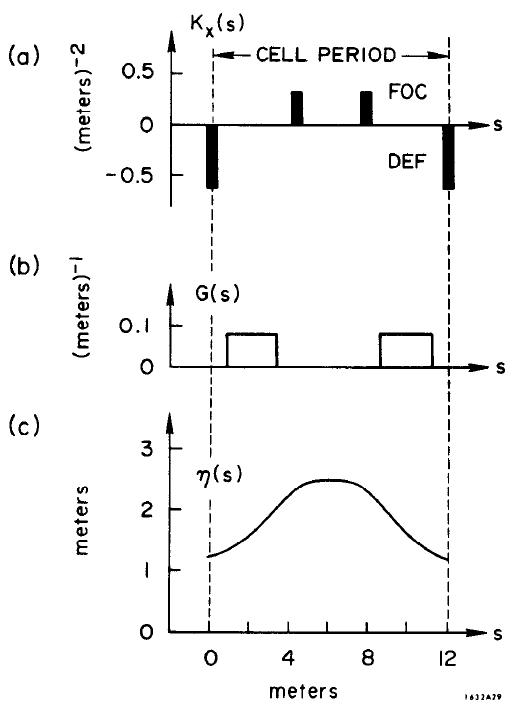
\includegraphics[width=0.6\linewidth]{./Figuras/fig29.jpeg}
	\caption{Funções do campo guia e a função de dispersão. Retirado de \cite{sands1970physics}.}
	\label{fig:fig29}
\end{figure}

Numa seção livre de campo, tanto $G$ quanto $K_x$ são nulas, então $\eta(s)$ tem um segmento com inclinação constante. Num quadrupolo puro, $G$ é zero e $K_x$ é apenas a força do quadrupolo. Num quadrupolo focalizador, $K_x$ é positivo e $\eta(s)$ segue uma oscilação senoidal em torno de zero na forma
\begin{align}
	\eta = a\ cos\left(\sqrt{K_x}s + \vartheta\right)
\end{align}
Em um quadrupolo desfocalizador, $K_x$ é negativo e $\eta(s)$ segue uma exponencial positiva na forma
\begin{align}
	\eta = a\ e^{(\sqrt{-K_x}s + \vartheta)}
\end{align}
A curva de $\eta(s)$ é "atraída" para o eixo $s$ em um quadrupolo focalizador e repelida do eixo em um quadrupolo desfocalizador.

Apesar de $K_1$ ser zero em um dipolo, $K_x$ não é. Na verdade, $K_x=G^2$ e a equação para $\eta$ fica
\begin{align}
	\eta'' = -G^2\eta + G = -G^2\left(\eta - \frac{1}{G}\right)
\end{align}

A curva de $\eta$ é um segmento senoidal o qual é "atraído" para $\eta_0 = 1/G$ com uma "força restauradora" proporcional a $G^2$ ($\eta_0$ é igual ao raio de curvatura $\rho$ da órbita ideal).

Da discussão acima, pode-se entender as características qualitativas das variações de $\eta(s)$ representadas na \autoref{fig:fig29}. Para todos os anéis de armazenamento "normais", a função de dispersão é positiva em todo o anel.

Considerando um campo guia de função separável, pode-se expandir a discussão anterior para calcular $\eta(s)$. Suponha que o cálculo inicie em $s=0$ assumindo alguns valores para $\eta(0)$ e $\eta'(0)$ e $\eta$ seja avaliada como uma sucessão de segmentos do tipo descrito anteriormente, até que seja feita uma revolução completa --  ou seja, até $s=L$. A verdadeira $\eta(s)$ será obtida se $\eta(0)$ e $\eta'(0)$ forem escolhidos de forma que $\eta(0) = \eta(L)$ e $\eta'(0) = \eta'(L)$. O cálculo pode ser computado utilizando uma técnica matricial.

A função de dispersão também pode ser obtida (para qualquer tipo de campo) utilizando os resultados obtidos na \autoref{sec:2.10} para as órbitas fechadas com distúrbio. Pode-se imaginar que a órbita fechada causada pela variação de energia é apenas uma órbita fechada com distúrbio, uma vez que tanto o desvio de energia quanto o erro de campo causam uma mudança na curvatura da trajetória. Em outras palavras, um erro de campo $\delta G$ em um segmento de órbita $\Delta s$ produz uma mudança na curvatura da trajetória de um elétron com energia $E_0$, mudança esta que é a mesma mudança na curvatura resultante de um desvio de energia $\epsilon$ de um elétron que viaja ao longo do campo nominal, já que $\delta G/G = \epsilon/E_0$. Já que $\eta(s)$ é a taxa do desvio da órbita fechada para $\epsilon/E_0$, pode-se computar $\eta(s)$ substituindo $\delta G$ na equação \eqref{eq:2.92} da \autoref{sec:2.11} por $G$. Este argumento também pode ser justificado notando que a equação \eqref{eq:3.4} para $\eta$ tem a mesma forma da equação \eqref{eq:2.85} para $x_c$ na \autoref{sec:2.10}; informalmente pode-se substituir $x_c \rightarrow \eta$ e $\delta G \rightarrow -G$. Fazendo estas substituições na equação \eqref{eq:2.94}, tem-se
\begin{align}
	\eta(s) = \frac{\sqrt{\beta(s)}}{2sen(\pi\nu)}\int\limits_{0}^{L}G(\bar{s})\sqrt{\beta(\bar{s})}cos(|\varphi(s)-\varphi(\bar{s})|-\pi\nu)d\bar{s}
\end{align}
Então, se $\beta(s)$ já é conhecido, pode-se obter $\eta(s)$ por uma integração. Note que $\eta(s)$ também terá um comportamento ressonante quando $\nu$ se aproxima de um inteiro.

Se a órbita ideal não está em um plano, esta discussão deve ser repetida para os desvios verticais. Neste caso, existirão duas funções de curvatura $G_x$ e $G_z$ assim como duas funções de focalização $K_x$ e $K_z$. Os desvios verticais também terão contribuições relativas ao desvio de energia, as quais serão proporcionais a função de dispersão $\eta_z(s)$. E a função de dispersão vertical pode ser avaliada em termos das funções de focalização e curvatura verticais. Terá apenas uma diferença qualitativa importante do caso horizontal: $\eta_z(s)$ terá tanto valores positivos quanto negativos, e sua média ao redor do anel será zero.
	\subsection{Tamanho da órbita: compactação de momento}\label{sec:3.2}
\begin{align}
	\mean{\eta}_{mag} = \frac{1}{\ell_{mag}}\int\limits_{mag}^{}\eta(s)ds\label{eq:3.13}
\end{align}
\begin{align}
	\alpha = \frac{2\pi}{L}\mean{\eta}_{mag} = \frac{\mean{\eta}_{mag}}{R}\label{eq:3.14}
\end{align}
\begin{align}
	\frac{\delta T}{T_0} = \frac{\delta \ell_\epsilon}{L} = \alpha \frac{\epsilon}{E_0}\label{eq:3.15}
\end{align}
	\subsection{Aproximação para órbita fechada e fator de compactação de momento}\label{sec:3.3}
Para campos guias mais práticos, existe uma relação próxima entre a função de dispersão $\eta(s)$ e a função betatron radial $\beta_x(s)$ a qual foi o foco em análises anteriores. Como a demonstração desta conexão é um pouco longa, ela não será feita aqui, apenas seu resultados serão apresentados. Para um campo guia isomagnético que possui uma função betatron bem comportada (sem variações bruscas), uma boa aproximação para $\eta(s)$ é
\begin{align}
	\eta(s) \approx a_0 \beta_x^{1/2}(s) = a_o \zeta(s)\ \ (isomag.)\label{eq:3.16}
\end{align}
onde $a_0$ é uma constante. Exceto pelo fator de escala $a_0$, a função $\eta(s)$ tem uma forma muito próxima à forma de $\zeta(s)$. Essa similaridade pode ser confirmada pelo menos para um caso comparando as Figuras \ref{fig:fig18} e \ref{fig:fig29} que mostram $\zeta_x(s)$ e $\eta(s)$ para um mesmo campo guia ilustrativo. Para este exemplo, a equação \eqref{eq:3.16} é uma boa aproximação.

Para a maioria das aplicações, será suficiente tomar $a_0$ como a relação entre as duas funções conhecidas. A equação que vem a partir da derivação matemática da equação \eqref{eq:3.16} é
\begin{align}
	a_0 = \frac{\mean{\beta_x^{1/2}}_{mag}}{\nu_x}\ \ (isomag.)\label{eq:3.17}
\end{align}
onde $\nu_x$ é a sintonia horizontal e a média magnética de $\beta_x^{1/2}$ é definida da mesma forma como foi definida para $\eta$ na análise anterior -- veja a equação \eqref{eq:3.13}.

O fator de escala $a_0$ também pode ser expresso em função dos parâmetros do anel definidos anteriormente. Analisando a média de ambos os lados da equação \eqref{eq:3.16} em todos os magnetos, tem-se que
\begin{align}
	\mean{\eta}_{mag} \approx a_0 \mean{\beta_x^{1/2}}_{mag}\ \ (isomag.)
\end{align}
Pela equação \eqref{eq:3.15}, o lado esquerdo da equação é apenas $\alpha R$ e pela equação \eqref{eq:3.17} o lado direito é apenas $a_0^2 \nu_x$, então
\begin{align}
	a_0^2 \approx \frac{\alpha R}{\nu_x}
\end{align}
e $\eta(s)$ pode ser escrito como
\begin{align}
	\eta(s) \approx \left(\frac{\alpha R}{\nu_x}\right)^{1/2}\beta_x^{1/2}(s)\label{eq:3.21}
\end{align}
Esta aproximação geralmente será uma representação adequada de $\eta(s)$.

Uma aproximação mais grosseira de $a_0$ pode ser obtida notando que, falando de forma geral, a média de $\beta_x^{1/2}$ nos ímãs é aproximadamente igual a raíz quadrada do valor típico de $\beta_x$ -- que foi definido anteriormente como $\beta_{xn} = R/\nu_x$ (veja a equação \eqref{eq:2.72}). Entção, utilizando a equação \eqref{eq:3.17}, espera-se que
\begin{align}
	a_0^2 \approx \frac{R}{\nu_x^3}
\end{align}

Os dois últimos resultados mostram uma conexão útil entre a sintonia $\nu_x$ e o fator de compactação de momento $\alpha$ dada por
\begin{align}
	\alpha \approx \frac{1}{\nu_x^2}
\end{align}
Esta simples conexão entre $\alpha$ e $\nu_x$ é útil para entender as características gerais dos anéis de armazenamento de alta energia. Considerando $\nu_x$ como a medida da "força" de focalização do campo guia, o fator de compactação de momento diminui com o inverso do quadrado da força.
	\subsection{Ganho e perda de energia}
Até agora, foram ignorados os efeitos os quais mudam a energia de um elétron armazenado; agora é necessário considerar estes processos onde um elétron ganha ou perde energia. A aceleração lateral ao longo das partes curvas da trajetória faz com que um elétron irradie uma parte da sua energia. As características desta perda por radiação serão discutidas mais a fundo na \autoref{sec:4.1}. Se um elétron deve permanecer capturado no anel de armazenamento, esta perda por radiação deve ser compensada por, na média, um ganho de energia equivalente proporcionado pelo sistema de aceleração de radiofrequência do anel -- um ou mais eletrodos os quais produzem, ao longo de algumas partes da órbita, um campo elétrico que carrega o elétron em movimento. É a ação combinada da perda por radiação com o ganho de energia -- juntamente com as propriedades do campo guia -- que garante a estabilidade dos \textit{bunches} armazenados, além de também ser responsável pelas pequenas oscilações de energia dos elétrons de um \textit{bunch}.

Um elétron com energia nominal $E_0$, movendo-se na órbita ideal, irá irradiar uma certa quantidade de energia, diga-se $U_0$, a cada revolução. Essa perda por radiação será sempre uma epquena fração da energia do elétron (tipicamente da ordem de $10^{-4}$ ou menos). E o ganho de energia do sistema de aceleração é, claro, da mesma ordem de magnitude. A pequena magnitude da perda por radiação em uma revolução permite algumas simplificações na sua análise. Para começar, pode-se aproximar que o elétron que começa uma revolução com energia $E_0$ irá perder a energia $U_0$ em uma revolução. Apesar de que a energia não permanecerá exatamente em $E_0$, nem a trajetória permanecerá na órbita ideal, os desvios em uma revolução podem ser desprezados. Com tudo, os efeitos cumulativos após várias revoluções devem ser levados em consideração.

Se o movimento de um elétron com energia $E_0$ segue uma oscilação betatron, sua taxa instantânea de perda de energia pode mudar -- devido à variação da aceleração lateral ao longo da trajetória. Mas a perda de energia média em uma revolução não irá sofrer alteração para uma aproximação de primeira ordem da amplitude da oscilação. Em outras palavras, mudanças na aceleração lateral são proporcionais a $x$ e irão, considerando apenas termos de primeira ordem, ter média zero em um ciclo completo. Já que basta considerar apenas os efeitos cumulativos de várias oscilações betatron, é necessário apenas analisar a média da perda de energia. Continuando com a análise linear do anel de armazenamento, qualquer dependência entre a perda por radiação e os desvios betatron pode ser ignorada.

No entanto, a perda por radiação irá variar com a variação da energia do elétron. Tanto uma variação na trajetória quanto na energia pode contribuir para uma alteração na perda de energia. Como toda variação de energia é lenta, pode-se considerar que um elétron está se movendo a todo instante na órbita fechada correspondente à sua energia instantânea -- ou está sofrendo oscilações betatron ao redor desta órbita. Como esta órbita fechada já é conhecida, pode-se computar a perda de energia em uma revolução. Por agora, pode-se considerar a perda de energia $U_{rad}(\epsilon)$ é uma função do desvio de energia $\epsilon$.

Como apenas pequenos desvios de energia estão sob análise, pode-se manter apenas termos de primeira ordem ao expandir a função em série de Taylor. Avaliando a expansão em $\epsilon=0$ -- ou seja, em $E=E_0$ -- tem-se que
\begin{align}
	U_{rad} = U_0 + D\epsilon\label{eq:3.23}
\end{align}
onde
\begin{align}
	D = \left(\frac{d\ U_{rad}}{d\ \epsilon}\right)_0
\end{align}
Neste momento, a perda por radiação é descrita pelas constantes $U_0$ e $D$ -- as quais serão avaliadas em termos das propriedades do campo guia na \autoref{sec:4}.

Agora, foque a análise para o sistema de aceleração de radiofrequência -- o sistema de RF, para facilitar -- o qual fornece energia aos elétrons para compensar a perda por radiação. O sistema de RF consiste de uma ou mais cavidades ressonantes, como a que está representada na \autoref{fig:fig30}, situadas em várias partes do anel e alimentadas com uma tensão de RF advinda de fontes de RF sincronizadas. estas cavidades produzem campos elétricos oscilantes ao longo da trajetória dos elétrons; e é a componente destes campos ao longo do caminho do elétron que carrega sua energia. Um elétron que completa um ciclo na órbita ideal é carregado pela cavidade de Rf com uma energia $U_0$ igual a integral da força elétrica instantânea ao longo da sua trajetória.

\begin{figure}[!htb]
	\centering
	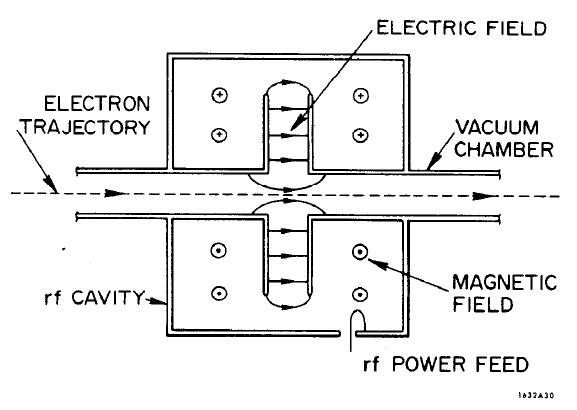
\includegraphics[width=0.7\linewidth]{./Figuras/fig30.jpeg}
	\caption{Diagrama esquemático de uma cavidade de RF. Retirado de \cite{sands1970physics}.}
	\label{fig:fig30}
\end{figure}

Como os campos de RF variam com o tempo, a energia recebida por um elétron em uma revolução depende do tempo em que este elétron passou pela cavidade de RF. Suponha que a dependência temporal do campo elétrico é dada. Então a energia $U_{RF}$ recebida por um elétron em uma revolução irá depender do tempo $\bar{t}$ em que ele começou sua revolução (considerando uma coordenada $s$ de referência, suponha $s=0$).

Se os elétrons devem ser armazenados próximos à órbita ideal, a variação de $U_{RF}(\bar{t})$ deve possuir algumas características. Primeiramente, assume-se que $U_{RF}(\bar{t})$ é uma função periódica com um período submúltiplo de $T_0$, o período de uma revolução de um elétron circulando na órbita ideal. Ou seja,
\begin{align}
	U_{RF}(\bar{t}+T_0/k) = U_{RF}(\bar{t})\label{eq:3.25}
\end{align}
onde $k$ é um inteiro chamado de número harmônico do sistema de RF. A variação de $U_{RF}(\bar{t})$ pode ser, por exemplo, como a curva representada na \autoref{fig:fig31} (apesar da suposição sobre a variação temporal de $U_{RF}$ ser mais restritiva que o necessário, os campos de RF devem ter pelo menos características similares para que o anel de armazenamento funcione).

\begin{figure}[!htb]
	\centering
	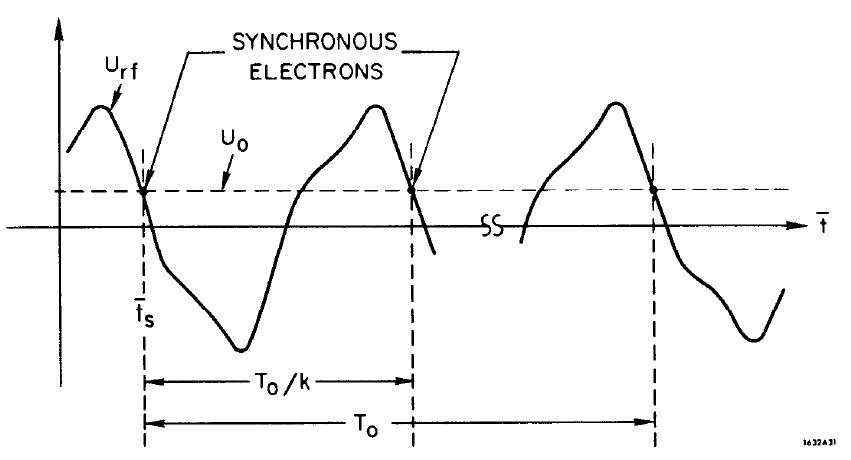
\includegraphics[width=0.85\linewidth]{./Figuras/fig31.jpeg}
	\caption{Ganho de energia do sistema de RF como uma função do tempo inicial $t$ de uma revolução. Retirado de \cite{sands1970physics}.}
	\label{fig:fig31}
\end{figure}

Agora, considere o que pode acontecer com um elétron com energia nominal $E_0$ circulando pela órbita ideal. Suponha que sua trajetória iniciou em $\bar{t}_s$, exatamente o tempo em que $U_{RF}(\bar{t}_s) = U_0$. Veja a \autoref{fig:fig31}. Na próxima revolução, perda e ganho de energia irão se compensar e o elétron irá retornar para seu ponto inicial novamente com energia $E_0$. O tempo necessário para uma revolução é $T_0$: então o elétron irá começar a próxima revolução no tempo $\bar{t}_s + T_0$ e, pela equação \eqref{eq:3.25}, o ganho de RF será novamente igual a $U_0$. O elétron irá continuar circulando pela órbita ideal indefinidamente. Este elétron o qual passa a coordenada de referência em $\bar{t}_s+jT_0$ (onde $j=1,2,3,...$) é chamado de elétron síncrono -- porque sua rotação está sincronizada com os campos de RF oscilantes. E $\bar{t}_s$ é chamada de fase síncrona do sistema de RF (é claro que com um sistema de Rf periódico existem tempos de início síncronos equivalentes para cada período de RF).

Foi assumido que o valor de pico de $U_{RF}$ é maior que a perda por radiação $U_0$ de um elétron síncrono. Disso, segue que existem ao menos duas escolhas possíveis de $\bar{t}_s$ em cada ciclo de $U_{RF}$ -- um onde $U_{RF}$ é crescente e outro onde ela é decrescente. Apenas um dos dois -- aquele onde $U_{RF}$ decresce -- corresponde a um movimento estável, como será mostrado. Então apenas este será designado como a fase síncrona $\bar{t}_s$. Pela \autoref{fig:fig31} também pode-se observar que com um número harmônico $k$ existem $k$ tempos síncronos de início diferentes -- e, desta forma, $k$ elétrons síncronos. Estas $k$ fases síncronas correspondem aos $k$ possíveis \textit{bunches}de elétrons armazenados no anel.

Um elétron movendo-se com um deslocamento lateral com relação á órbita ideal irá ver um campo elétrico diferente do campo visto por um elétron na órbita ideal. Porém, geralmente o ganho de energia em uma revolução depende muito pouco do deslocamento lateral. Sendo assim, é razoável ignorar qualquer dependência do ganho de energia com o deslocamento lateral -- independente se este for causado por oscilações betatron ou de energia -- e considerar apenas a variação do ganho de energia com o tempo de início $\bar{t}$.

A posição circular do elétron síncrono prevê um ponto de referência conveniente para o estudos das oscilações longitudinais de um elétron em um \textit{bunch}. De fato, esta posição  do elétron síncrono é referenciada como sendo o "centro"  do \textit{bunch} e descreve a posição azimutal instantânea de qualquer outro elétron do \textit{bunch} em função do seu deslocamento longitudinal $y$ a partir do centro do \textit{bunch}. Isto é, define-se
\begin{align}
	y(t) = s(t) - s_c(t)
\end{align}
onde $s$ é a posição azimutal de qual elétron em particular e $s_c$ refere-se a posição do centro do \textit{bunch}. Veja a \autoref{fig:fig32}.

\begin{figure}[!htb]
	\centering
	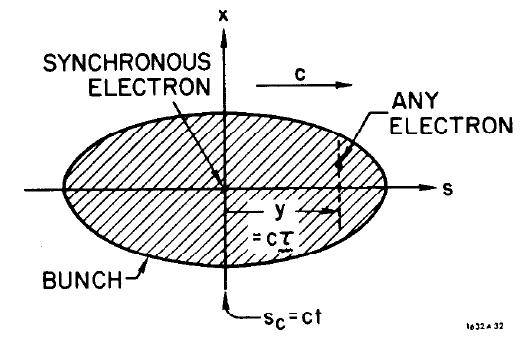
\includegraphics[width=0.6\linewidth]{./Figuras/fig32.jpeg}
	\caption{Coordenadas longitudinais $y$ e $\tau$ de um elétron em um \textit{bunch}. Retirado de \cite{sands1970physics}.}
	\label{fig:fig32}
\end{figure}

Para a presente discussão, é conveniente descrever o movimento longitudinal por uma variável equivalente $\tau$ definida simplesmente como
\begin{align}
	\tau(t) = y(t)/c
\end{align}
e chamada de deslocamento temporal do centro do \textit{bunch}. O deslocamento temporal é muito próximo do intervalo de tempo $\Delta t$ entre a chegada de um elétron em qualquer coordenada $s$ em particular e a chegada do elétron síncrono nesta mesma coordenada. A diferença é igual a mudança em $\tau$ no tempo $\Delta t = \tau$, a qual pode ser ignorada devido a lenta variação de $\tau$. note que o deslocamento temporal $\tau$ é positivo quando um elétron chega em cada coordenada $s$ antes do elétron síncrono.

Devido às variações temporais dos campos elétricos do sistema de RF, apenas um elétron síncrono irá receber a energia $U_0$ em uma revolução. Qualquer outro elétron irá ganhar uma energia $U_{RF}$ que depende do deslocamento temporal $\tau$. Utilizando a notação convencional, escreve-se
\begin{align}
	U_{RF} = eV(\tau)
\end{align}
onde $e$ é a carga do elétron e $V(\tau)$ é chamada de "tensão de RF" -- em analogia a um sistema de aceleração DC. A forma de $V(\tau)$ é, claro, relacionada a $U_{RF}$; especificamente,
\begin{align}
	eV(\tau) = U_{RF}(\bar{t}_s - \tau)
\end{align}
A variação com relação a $\tau$ é contrário à variação com $\bar{t}$, então a função de ganho de energia dada pela \autoref{fig:fig31} corresponde à função $V(\tau)$ dada pela \autoref{fig:fig33} -- onde, agora, $\tau=0$ corresponde ao deslocamento temporal de um elétron síncrono. Note que a inclinação de $V(\tau)$ é positiva em $\tau=0$.

\begin{figure}[!htb]
	\centering
	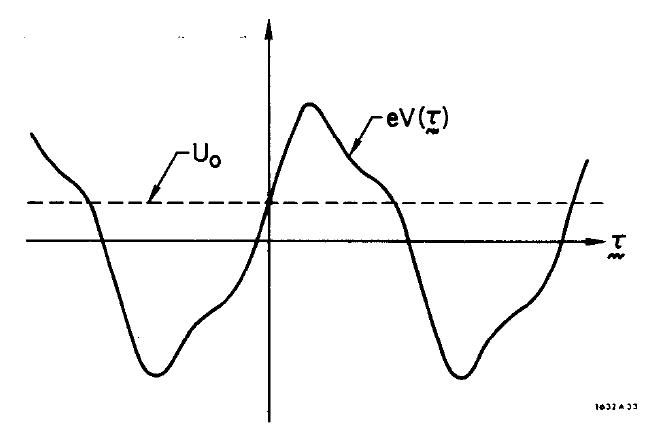
\includegraphics[width=0.6\linewidth]{./Figuras/fig33.jpeg}
	\caption{Função da tensão de RF $V(\tau)$. Retirado de \cite{sands1970physics}.}
	\label{fig:fig33}
\end{figure}

É pertinente enfatizar o fato de que a "tensão" efetiva de múltiplas cavidades de RF de anéis de armazenamento de alta energia não é simplesmente relacionada com alguma "tensão" elétrica observável, mas esta sim depende das posições relativas e fases de oscilação das várias cavidades de Rf do sistema. A tensão $V(\tau)$ depende, na verdade, do sentido de circulação da partícula ao redor do anel e, sendo assim, pode ser diferente para elétrons circulando em um sentido ao redor do anel e positróns circulando no sentido contrário.

Agora, as oscilações de energia de um elétron em um \textit{bunch} circulando no anel de armazenamento estão prontas para serem consideradas. Primeiramente, pode-se fazer uma análise qualitativa do que irá acontecer. Suponha que o elétron comece com energia nominal $E_0$, mas com um deslocamento temporal positivo $\tau$ -- desta forma, o elétron está à frente da posição síncrona. A perda por radiação depende apenas da energia, então ela será $U_0$ a cada revolução. Mas o ganho de energia será maior que $U_0$, uma vez que o elétron está adiantado com relação ao elétron síncrono. Este elétron ganhará um pouco mais de energia a cada revolução. Mas um aumento na sua energia irá, pela equação \eqref{eq:3.15}, causar um aumento no seu período de revolução; e seu avanço de tempo com relação ao centro do \textit{bunch} irá, portanto, começar a diminuir. Após algumas revoluções, o deslocamento temporal chegará a zero. Mas, quando isto acontecer, a energia do elétron será maior que a energia nominal $E_0$ -- já que ele esteve ganhando energia continuamente -- então seu deslocamento temporal continuará diminuindo, agora assumindo valores negativos de $\tau$. No entanto, em valores negativos de $\tau$, o ganho de energia será muito pequeno para compensar a perda de energia por radiação e a energia do elétron irá começar a diminuir em direção à energia nominal $E_0$. Quando a energia nominal for atingida, o deslocamento temporal irá parar de diminuir mas, como $\tau$ é negativo, o ganho de energia por revolução é menor que $U_0$ e a energia irá começar a decrescer, ficando menor que $E_0$. Agora o deslocamento temporal irá começar a aumentar, voltando para zero. O processo irá continuar até que $\tau$ retorne ao seu valor inicial, onde a energia será novamente $E_0$.

Analisando agora de forma quantitativa. Primeiramente, analise a variação do deslocamento temporal $\tau$. É conveniente analisar o que está acontecendo observando um \textit{bunch} a cada revolução quando o centro do \textit{bunch} está em alguma coordenada de referência. A discussão é facilitada tomando esta coordenada de referência em um ponto sem nenhum campo (longe de ímãs ou cavidades de RF). Na \autoref{fig:fig34} estão contidas duas "fotos" do mesmo \textit{bunch} em duas passagens consecutivas pela coordenada de referência. Em cada foto o centro do \textit{bunch} está na coordenada de referência, então o tempo entre as imagens é apenas $T_0$ --  o tempo de uma revolução pela órbita ideal.

\begin{figure}[!htb]
	\centering
	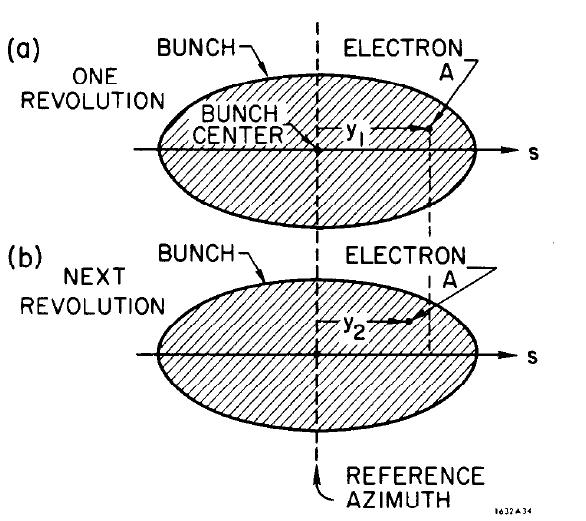
\includegraphics[width=0.6\linewidth]{./Figuras/fig34.jpeg}
	\caption{Movimento longitudinal de um elétron em um \textit{bunch}. Retirado de \cite{sands1970physics}.}
	\label{fig:fig34}
\end{figure}

As imagens também mostram a posição de um elétron em particular: "Elétron A". Na primeira imagem, o Elétron A está à frente do centro do \textit{bunch} de uma distância $y_1$. Na segunda imagem, o deslocamento longitudinal decaiu para $y_2$. Entre as duas "fotos", o centro do \textit{bunch} percorreu uma volta ao longo da órbita ideal, ou seja, uma distância $L=cT_0$. E, como o Elétron A também viaja na velocidade da luz $c$, este também percorreu uma distância $L$. Mas, se este elétron possui um desvio de energia $\epsilon$, foi mostrado na \autoref{sec:3.2} que o comprimento de uma revolução completa será maior que $L$ por uma quantidade $\delta \ell$ dada por
\begin{align}
	\frac{\delta \ell}{L} = \alpha\frac{\epsilon}{E_0}
\end{align}
Note que para $\epsilon$ positivo -- ou seja, $E>E_0$ -- $\delta \ell$ também é positivo, o que implica que o caminho a ser percorrido pelo elétron fica maior. Pois bem, desta forma o Elétron A não consegue alcançar sua coordenada anterior $y_1$ por uma pequena distância $\delta y = -\delta \ell$, ou seja,
\begin{align}
	y_2 - y_1 = \delta y = -\alpha \frac{\epsilon}{E_0}L
\end{align}
A variação de $\tau$ em uma revolução é
\begin{align}
	\delta \tau = \frac{\delta y}{c} = -\alpha \frac{\epsilon}{E_0}\frac{L}{c} = -\alpha\frac{\epsilon}{E_0}T_0
\end{align}
Como o tempo entre cada imagem é $T_0$, a taxa de variação temporal de $\tau$ é apenas $\delta \tau/T_0$, ou ainda
\begin{align}
	\frac{d \tau}{dt} = -\alpha \frac{\epsilon}{E_0}\label{eq:3.32}
\end{align}

Agora, a variação da energia. Durante sua revolução, o Elétron A perdeu uma parte $U_{rad}(\epsilon)$ da sua energia, e ganhou da cavidade de RF $eV(\tau_1)$. A variação da energia nesta revolução é, portanto,
\begin{align}
	\delta U = eV(\tau)-U_{rad}(\epsilon)
\end{align}
A taxa de variação do desvio de energia $\epsilon$ -- avaliada em uma revolução completa -- é $\delta U/T_0$, então tem-se que
\begin{align}
	\frac{d\epsilon}{dt} = \frac{eV(\tau)-U_{rad}(\epsilon)}{T_0}\label{eq:3.34}
\end{align}

Combinando as equações \eqref{eq:3.32} e \eqref{eq:3.34}, pode-se descrever as oscilações de energia -- e as oscilações temporais associadas --  de um elétron armazenado. É preciso resolver as duas equações juntas para obter a variação de $\epsilon$ e $\tau$ com relação ao tempo.

Infelizmente, os deslocamentos temporais associados a pequenas variações de energia não são necessariamente pequenos no sentido de eles podem abranger uma fração significante de um ciclo completo de variação de $V(\tau)$. Apenas neste caso não é possível considerar apenas os termos lineares durante a análise. Talvez seja necessário computar as variações não-lineares de $V(\tau)$. Nos casos em que uma pequena variação da energia causa um deslocamento temporal é pequeno, entretanto, pode-se considerar apenas os termos lineares da variação de $V(\tau)$. Já que o ganho de energia para $\tau=0$ é, por definição, $U_0$, ao expandir a função em série de Taylor tem-se que
\begin{align}
	U_{RF} = eV(\tau) = U_0 + e\dot{V}_0\tau\label{eq:3.35}
\end{align}
onde $\dot{V}_0$ é $dV/d\tau$ avaliada em $\tau=0$.

É comum que a tensão de Rf em um anel de armazenamento tenha uma variação senoidal com relação ao tempo. Nestes casos, tem-se que a tensão é descrita por
\begin{align}
	V(\tau) = \widehat{V}\ sen(\omega_{RF}(\tau+\tau_0))
\end{align}
onde $\widehat{V}$ é chamado de valor de pico da tensão de RF e $\omega_{RF}\tau_0$ é chamada de fase síncrona de RF. De acordo com as suposições feitas,
\begin{align}
	\omega_{RF} = 2\pi \frac{k}{T_0} = k\omega_r
\end{align}
onde $\omega_r$ é a frequência angular de uma revolução. Também segue que
\begin{align}
	\omega_{RF}\tau_0 = sen^{-1}(U_0/e\widehat{V})
\end{align}
e
\begin{align}
	\dot{V}_0 = \omega_{RF}\widehat{V}cos(\omega_{RF}\tau_0) = \omega_{RF}\widehat{V}\left[1-\left(\frac{U_0}{e\widehat{V}}\right)^2\right]^{1/2}
\end{align}

\begin{proof}
	Pela equação \eqref{eq:3.25}, o período da função $U_{RF}$ é $T_0/k$. Logo, sua frequência é $k/T_0$. Logo, sua frequência angular é
	\begin{align*}
		\omega_{RF} = 2\pi f_{RF} = 2\pi \frac{k}{T_0}
	\end{align*}
	Mas $2\pi \frac{1}{T_0}$ é a frequência angular de uma revolução completa. Logo, $\omega_{RF} = k\omega_r$.
	
	Agora, seja a tensão de RF dada por $V(\tau) = \widehat{V}\ sen(\omega_{RF}(\tau+\tau_0))$. Logo, $V(0) = \widehat{V}\ sen(\omega_{RF}\tau_0)$. Sendo assim, avaliando a equação \eqref{eq:3.35} em $\tau=0$, tem-se que
	\begin{align*}
		e\widehat{V}\ sen(\omega_{RF}\tau_0) &= U_0\\
		\therefore \omega_{RF}\tau_0 &= sen^{-1}(U_0/e\widehat{V})
	\end{align*}
	Por fim, derivando a expressão de $V(\tau)$, tem-se
	\begin{align*}
		\frac{dV}{d\tau} &= \omega_{RF}\widehat{V}\ cos(\omega_{RF}(\tau+\tau_0))\\
		\therefore \widehat{V}_0 = \left(\frac{dV}{d\tau}\right)_0 &= \omega_{RF}\widehat{V}\ cos(\omega_{RF}(\tau_0))
	\end{align*}
	Mas, pela relação trigonométrica $sen^2(x) + cos^2(x) = 0$, tem-se que
	\begin{align*}
		cos(\omega_{RF}\tau_0) = [1-sen^2(\omega_{RF}\tau_0)]^{1/2}\\
		\therefore \widehat{V}_0 = \omega_{RF}\widehat{V}[1-sen^2(\omega_{RF}\tau_0)]^{1/2}
	\end{align*}
	Porém, já foi demonstrado aqui que $\omega_{RF}\tau_0 = sen^{-1}(U_0/e\widehat{V})$. Substituindo esta relação, tem-se que
	\begin{align*}
		\therefore \widehat{V}_0 = \omega_{RF}\widehat{V}\left[1-\left(\frac{U_0}{e\widehat{V}}\right)\right]^{1/2}
	\end{align*}
	c.q.d.
\end{proof}
	\subsection{Pequenas oscilações}\label{sec:3.5}
Agora já é possível analisar com detalhe as oscilações de energia de um elétron em um \textit{bunch}. Primeiramente, a análise será feita para o caso em que pequenas oscilações de energia causam também pequenas oscilações no deslocamento temporal $\tau$, as quais ocorrem desde que sejam limitadas por um pequeno intervalo correspondente a um segmento aproximadamente linear de $V(\tau)$. Na \autoref{sec:3.6} serão analisadas as oscilações não-lineares que ocorrem quando as variações de $\tau$ são grandes.

Para pequenos $\tau$ e $\epsilon$, pode-se substituir $v(\tau)$ e $U_{rad}(\epsilon)$ por suas aproximações lineares (séries de Taylor) contidas nas equações \eqref{eq:3.35} e \eqref{eq:3.23}, respectivamente. Assim, a equação \eqref{eq:3.34} fica
\begin{align}
	\frac{d\epsilon}{dt} = \frac{1}{T_0}(e\dot{V}_0 \tau - D\epsilon)\label{eq:3.40}
\end{align}
Esta equação pode ser combinada com a equação \eqref{eq:3.32}, resultando em uma equação diferencial para $\epsilon$ e $\tau$. Escolhendo $\tau$, pode-se tomar a derivada da equação \eqref{eq:3.32} com relação ao tempo e eliminar $\epsilon$, obtendo-se
\begin{align}
	\frac{d^2 \tau}{dt^2} + 2\alpha_\epsilon \frac{d\tau}{dt} + \Omega^2 \tau = 0\label{eq:3.41}
\end{align}
onde
\begin{align}
	\alpha_\epsilon &= \frac{D}{2 T_0}\label{eq:3.42}\\
	\Omega^2 &= \frac{\alpha\ e\ \dot{V}_0}{T_0\ E_0}
\end{align}

Note que a equação \eqref{eq:3.41} descreve uma oscilação harmônica amortecida com frequência angular de oscilação $\Omega$ e coeficiente de amortecimento $\alpha_\epsilon$. Como a taxa de amortecimento em um anel é sempre lenta ($\alpha_\epsilon<<\Omega$), a solução da equação \eqref{eq:3.41} pode ser escrita como
\begin{align}
	\tau(t) = A\ e^{-\alpha_\epsilon t}\ cos(\Omega t - \theta_0)
\end{align}
com $A$ e $\theta_0$ são constantes arbitrárias. Ou, usando a notação complexa usual,
\begin{align}
	\tau(t) = \tilde{\tau}\ e^{-(\alpha_\epsilon - i\Omega)t}
\end{align}
onde $\tilde{\tau}$ é uma constante complexa.

\begin{proof}
	Seja a variação de $\tau$ dada pela equação diferencial $\frac{d^2 \tau}{dt^2} + 2\alpha_\epsilon \frac{d\tau}{dt} + \Omega^2 \tau = 0$. Esta é uma EDO homogênea de segunda ordem, a qual pode ser resolvida através de sua equação característica:
	\begin{align*}
		r^2 + 2\alpha_\epsilon r + \Omega^2 = 0
	\end{align*}
	Resolvendo esta equação do segundo grau, tem-se que
	\begin{align*}
		r = \frac{-2\alpha_\epsilon \pm \sqrt{(2\alpha_\epsilon)^2 - 4\Omega^2}}{2}
	\end{align*}
	Considerando que $\alpha_\epsilon << \Omega$, pode-se simplificar a solução por
	\begin{align*}
		r = -\alpha_\epsilon \pm \Omega i
	\end{align*}
	Para uma equação característica com solução complexa, a solução da EDO é dada por
	\begin{align*}
		\tau = c_1\ e^{\alpha_\epsilon t}\ cos(\Omega t) + c_2\ e^{\alpha_\epsilon t}\ sen(\Omega t)
	\end{align*}
	Como um seno nada mais é que um cosseno defasado de $\pi/2$, esta solução pode ser reescrita como
	\begin{align*}
		\tau = A\ e^{\alpha_\epsilon t}\ cos(\Omega t - \theta_0)
	\end{align*}
\end{proof}

As equações \eqref{eq:3.40} e \eqref{eq:3.32} também podem ser resolvidas para $\epsilon$, obtendo-se a mesma equação diferencial \eqref{eq:3.41}. Assim, a variação de $\epsilon$ com o tempo é
\begin{align}
	\epsilon(t) = \tilde{\epsilon}\ e^{-(\alpha_\epsilon - i\Omega)t}
\end{align}
Pela equação \eqref{eq:3.32}, $\tilde{\epsilon}$ e $\tilde{\tau}$ são relacionados da seguinte maneira:
\begin{align}
	\tilde{\epsilon} = -i\frac{\Omega E_0}{\alpha}\tilde{\tau}\label{eq:3.47}
\end{align}
(considerando $\alpha_\epsilon << \Omega$) e, desta forma, as oscilações de $\epsilon$ e $\tau$ terão uma diferença de fase de $\pi/2$.

Note que a frequência de oscilação de pequenas oscilações de energia depende do sistema de Rf apenas pelo termo $\dot{V}_0$. A frequência é proporcional à raiz quadrada da derivada da RF na fase síncrona. Os outros parâmetros -- $\alpha$, $T_0$ $E_0$ -- são característicos do campo guia (incluindo a energia na qual ele é operado). A constante de amortecimento $\alpha_\epsilon$ das oscilações de energia -- a qual é o inverso da constante de amortecimento no tempo -- é proporcional a $D$, a qual é a taxa de variação da perda de energia por radiação. Como será mostrado posteriormente, esta taxa depende da energia do elétron e das propriedades do campo guia.

Para ajudar na análise dos resultados obtidos, é importante ter uma noção da ordem de magnitude das variáveis estudadas. Sendo assim, para um anel de armazenamento de 1 GeV:
\begin{align*}
	\omega_r = 2\pi /T_0 &\approx 10^7 s^{-1}\\
	\omega_\beta = \nu \omega_r &\approx 3\omega_r\\
	\Omega &\approx 10^4 s^{-1}\\
	\alpha_\epsilon &\approx 10 s^{-1}
\end{align*}
Analisando as relações $\omega_r/\Omega$ e $\Omega/\alpha_\epsilon$ pode-se justificar as aproximações feitas.

Na ausência de amortecimento, $\epsilon$ e $\tau$ são variáveis conjugadas. No diagrama de fase de $\epsilon$ versus $\tau$, as oscilações são descritas por um ponto que se move ciclicamente por uma elipse. Veja a \autoref{fig:fig35}(a). A relação entre os dois eixos principais da elipse é -- pela equação \eqref{eq:3.47}
\begin{align}
	\frac{\epsilon_{max}}{\tau_{max}} = \frac{|\tilde{\epsilon}|}{|\tilde{\tau}|} = \frac{\Omega E_0}{\alpha}
\end{align} 

\begin{figure}[!htb]
	\centering
	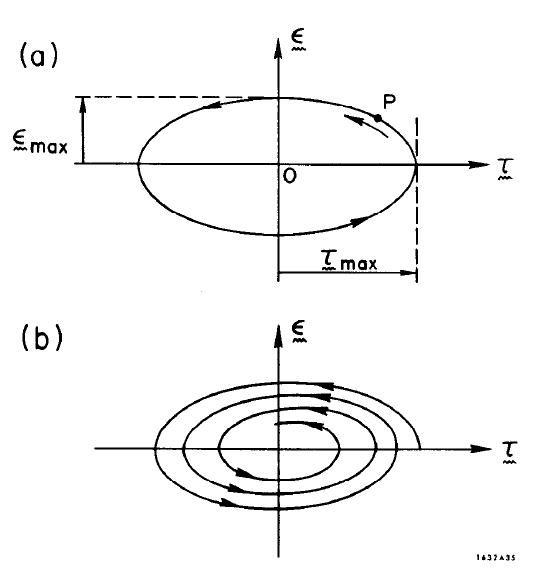
\includegraphics[width=0.6\linewidth]{./Figuras/fig35.jpeg}
	\caption{Diagrama de fase para as oscilações de energia. (a) Sem amortecimento. (b) Com amortecimento. (A taxa de amortecimento está bem exagerada). Retirado de \cite{sands1970physics}.}
	\label{fig:fig35}
\end{figure}

Se as escalas são escolhidas de forma que a elipse se torne um círculo, o ponto de referência rotaciona a uma frequência angular $\Omega$ constante. Com amortecimento, o tamanho da elipse decresce lentamente e a fase da trajetória é uma lenta espiral convergindo para o centro, como pode-se ver na \autoref{fig:fig35}(b). O diagrama de fase também mostra porque o amortecimento depende de $dU_{rad}/dE$. Se sua derivada é positiva, o elétron está perdendo uma quantidade extra de energia na metade superior da elipse, e ganhando uma quantidade extra de energia na metade inferior. Desta forma, o ponto de referência está sempre se dirigindo para o eixo $\tau$ e a amplitude de oscilação está diminuindo -- proporcionalmente a $dU_{rad}/dE$.

De acordo com a solução aqui proposta, as oscilações de energia de todos os elétrons deveriam ser completamente amortecidas em algum momento, fazendo com que todos os elétrons fiquem sobre o elétron síncrono. Mas ainda não foi considerada a excitação das oscilações causada por efeitos quânticos os quais "balançam" as oscilações e previnem que estas sejam completamente anuladas (estes efeitos serão considerados na \autoref{sec:4}). Em condições estacionárias, qualquer elétron armazenado será tipicamente encontrado com uma amplitude de oscilação residual na qual há um balanço entre a excitação e o amortecimento. Como ambos os processos são lentos, pode-se pensar que a oscilação de energia em qualquer curto período de tempo pode ser descrita por uma elipse fixa, como a representada na \autoref{fig:fig34}(a).

É importante ter em mente que as oscilações de energia estão relacionadas não só com as oscilações longitudinais (em $y$ ou $\tau$) dos elétrons em um \textit{bunch}, mas elas também possuem uma componente lateral. De acordo com a equação \eqref{eq:3.3}, o desvio de energia $\epsilon$ resulta em um deslocamento radial $x_\epsilon$ proporcional a $\epsilon$ -- e em fase com o mesmo. Então a componente $x_\epsilon$ do deslocamento horizontal total oscila em sincronia com as oscilações de energia. Em geral, esta manifestação transversal das oscilações de energia possui (em condições estacionárias) uma amplitude muito próxima das oscilações betatron.
	\subsection{Grandes oscilações: abertura dinâmica}\label{sec:3.6}
O campo guia de um anel de armazenamento normalmente aceita apenas uma pequena faixa de energias -- tipicamente só uma pequena porcentagem da energia nominal -- e as forças magnéticas focalizadoras são razoavelmente lineares em toda esta faixa de energia. No entanto, pequenos desvios de energia podem corresponder a grandes oscilações do deslocamento temporal $\tau$. Neste caso, grandes oscilações significam valores de $\tau$ onde $V(\tau)$ deixa de ter uma dependência linear com $\tau$. Estas grandes amplitudes ocorrem geralmente quando a tensão de pico de RF não é muito maior que a perda por radiação (que é o caso em altas energias) ou quando o número harmônico de RF $k$ é muito grande. Estas oscilações devem ser analisadas pois são elas as responsáveis por determinar a abertura dinâmica do anel. Mantenha em mente que, apesar de grandes oscilações temporais estarem sob análise, as oscilações de energia continuam pequenas.

Pois bem, da \autoref{sec:3.4} foram obtidas as equações \eqref{eq:3.32} e \eqref{eq:3.34}. Como foi feito antes, substitui-se $U_{rad}$ por $U_0 +D\epsilon$, já que as oscilações de energia são pequenas. Mas agora $V(\tau)$ não pode mais ser substituída por sua aproximação linear, então a equação \eqref{eq:3.34} fica
\begin{align}
	\frac{d\epsilon}{dt} = \frac{eV(\tau) - U_0}{T_0} - \frac{D\epsilon}{T_0}
\end{align}
Expressando $\epsilon$ e sua derivada com relação ao tempo em termos de $\tau$ pela equação \eqref{eq:3.32}, tem-se
\begin{align}
	\frac{d^2 \tau}{dt^2} = -\frac{\alpha}{E_0 T_0}[eV(\tau)-U_0] - \frac{D}{T_0}\frac{d\tau}{dt}\label{eq:3.49}
\end{align}
Esta equação descreve a variação de $\tau$ para qualquer amplitude.

É possível comparar a equação \eqref{eq:3.49} com uma equação bem conhecida:
\begin{align}
	m\frac{d^2x}{dt^2} = F(x) - \mu\frac{dx}{dt}\label{eq:3.50}
\end{align}
Esta equação representa o movimento unidimensional em $x$ de uma partícula com massa $m$, a qual se move em um campo de força conservativo $F(x)$ e sofre uma força de fricção proporcional à sua velocidade. Sendo assim, pode-se entender a equação \eqref{eq:3.49} por meio de uma comparação direta com a equação \eqref{eq:3.50}. O movimento em $\tau$ é exatamente igual ao movimento de uma partícula com massa unitária em um campo de força conservativo
\begin{align}
	F(\tau) = -\frac{\alpha}{E_0 T_0}[eV(\tau) - U_0]\label{eq:3.51}
\end{align}
sofrendo uma força de fricção proporcional à sua velocidade com um coeficiente $D/T_0$.

Geralmente, o movimento em $\tau$ pode ser avaliado apenas por computação numérica. No entanto, pode-se obter uma boa ideia heurística considerando o que acontece se o termo friccional é zero. Ele é mesmo pequeno e pode ser considerado como uma perturbação depois. Pois bem, deseja-se estudar o movimento
\begin{align}
	\frac{d^2\tau}{dt^2} = F(\tau)
\end{align}
onde $F(\tau)$ é dada pela equação \eqref{eq:3.51}. Este tipo de equação é geralmente resolvido definindo uma função de "energia potencial", a qual é o negativo da integral da força. Assim, define-se
\begin{align}
	\Phi(\tau) = \frac{\alpha}{E_0 T_0} \int\limits_{\tau}^{0}[eV(\bar{\tau}) - U_0]d\bar{\tau}
\end{align}
Agora o movimento pode ser analisado utilizando o princípio de conservação de energia. Em cada instante, a soma da "energia potencial" $\Phi(\tau)$ e da "energia cinética" -- dada por $\frac{1}{2}(d\tau/dt)^2$ -- deve ser constante, dada pela "energia total". A energia total também é o máximo $\Phi_0$ que pode ser alcançado por $\Phi(\tau)$ -- o qual irá ocorrer quando $d\tau/dt$ for zero. Logo, pode-se escrever que
\begin{align}
	\frac{1}{2}\left(\frac{d\tau}{dt}\right)^2 = \Phi_0 - \Phi(\tau)\label{eq:3.54}
\end{align}

Suponha que a função do ganho de energia $eV(\tau)$ tenha a forma representada na \autoref{fig:fig36}(a) e o ganho de energia síncrono $U_0$ também representado nesta figura. Então $\Phi(\tau)$ será como a curva representada na parte (b) da \autoref{fig:fig36}. A forma mostrada é razoavelmente típica. Note que $\Phi(\tau)$ tende a decrescer com uma inclinação média de $-U_0$. Isto precisa ocorrer pois a integral dos campos de aceleração de RF deve ser zero em um ciclo completo (pelo menos em um ciclo completo da menor frequência presente).

\begin{figure}[!htb]
	\centering
	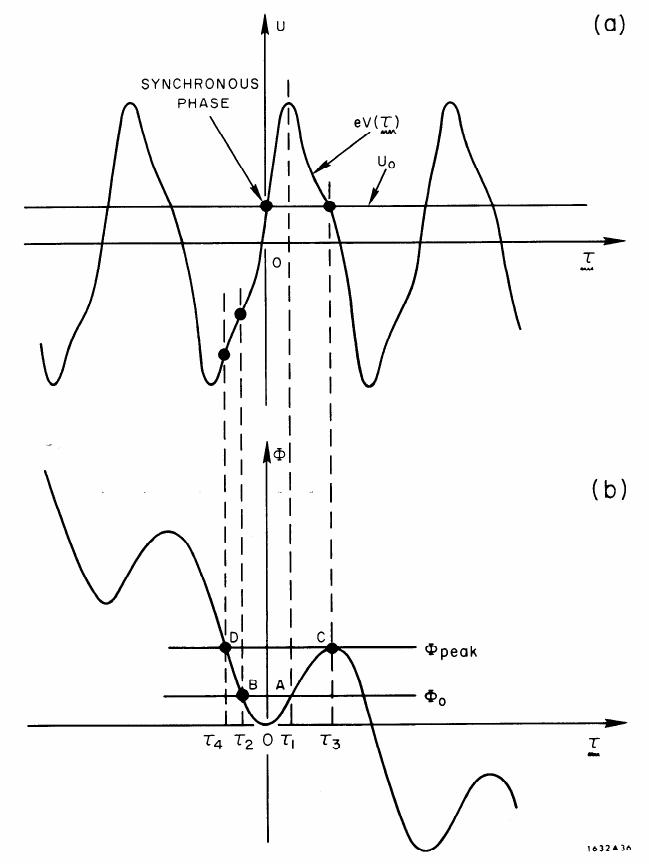
\includegraphics[width=0.9\linewidth]{./Figuras/fig36.jpeg}
	\caption{(a) Função de aceleração de RF $eV(\tau)$, e (b) a função da energia potencial efetiva $\Phi(\tau)$.}
	\label{fig:fig36}
\end{figure}

Agora a natureza das oscilações do deslocamento temporal pode ser visualizada. O movimento é parecido com o de uma partícula pontual (um "elétron") que se move "pela" superfície montanhosa representada por $\Phi(\tau)$ -- onde, é claro, você deve pensar em $\tau$ como sendo uma coordenada espacial horizontal. Primeiramente, existe um potencial mínimo em $\tau=0$. Se o elétron é posicionado neste ponto, ele permanece estacionário; este é o "elétron síncrono" \footnote{Existem, é claro, pontos estacionários em cada mínimo do potencial, e estes correspondem aos elétrons síncronos nos centros de outros \textit{bunches} (enquanto $\tau<T_0$).}. No entanto, se o elétron for posicionado em $\tau_1$ -- o ponto correspondente ao ponto $A$ na montanha -- ele irá descer pela montanha e para no ponto oposto B. A e B estão na mesma altura $\Phi_0 = \Phi(\tau_A)$. Em $\tau_A$ e $\tau_B$ a energia cinética é zero. A energia cinética irá atingir seu valor máximo quando o elétron passar $\tau=0$. Em cada $\tau$ a energia cinética é dada pela equação \eqref{eq:3.54} e a partir desta pode-se obter a "velocidade" em cada $\tau$:
\begin{align}
	\frac{d\tau}{dt} = \pm \sqrt{2}[\Phi_0 - \Phi(\tau)]^{1/2}
\end{align}

Lembre-se, agora, que pela equação \eqref{eq:3.32} a "velocidade" é dada por
\begin{align*}
	\frac{d\tau}{dt} = -\alpha \frac{\epsilon}{E_0}
\end{align*}
então o desvio de energia (de um elétron real) em cada $\tau$ é dado por
\begin{align}
	\frac{\epsilon(\tau)}{E_0} = + \frac{\sqrt{2}}{\alpha}[\Phi_0-\Phi(\tau)]^{1/2}\label{eq:3.56}
\end{align}

Esta relação pode ser facilmente vista em um diagrama de fase -- $\epsilon$ versus $\tau$ -- no qual quase uma elipse é obtida, semelhante à curva representada na \autoref{fig:fig37}. Deve-se apenas utilizar o senso comum para escolher o sinal apropriado da raiz quadrada para cada metade do ciclo.

\begin{figure}[!htb]
	\centering
	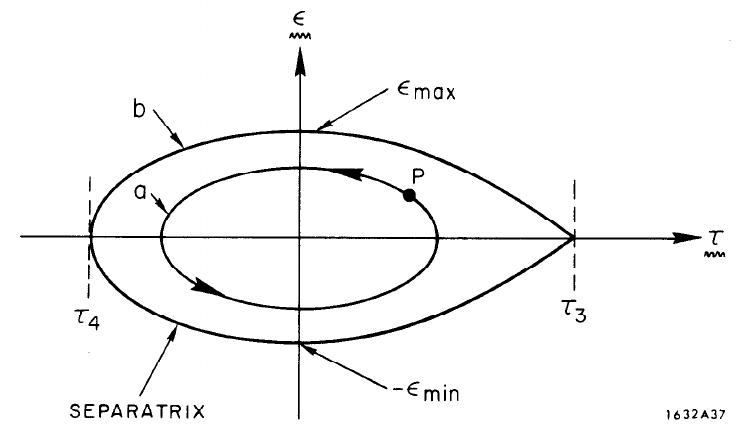
\includegraphics[width=0.7\linewidth]{./Figuras/fig37.jpeg}
	\caption{Diagrama de fase para grandes oscilações. Oscilações de energia limitadas ocorrem apenas dentro da separatriz.}
	\label{fig:fig37}
\end{figure}

Também pode-se ver o que acontece considerando o termo de fricção -- o amortecimento por radiação. Durante cada ciclo de oscilação, uma pequena quantidade de energia será perdida, resultando numa diminuição da "energia" total (pode-se estimar este valor se o movimento for aproximado por uma senoide).

Deve ser aparente que haverá uma amplitude máxima para as oscilações estáveis (periódicas) de $\tau$. Ela ocorre quando o elétron atinge o pico da montanha em $\tau_3$ -- correspondente ao ponto C da \autoref{fig:fig36}(b) -- onde $\Phi(\tau)$ é $\Phi_{max}$. Um elétron com qualquer amplitude maior irá passar o pico da montanha e adentrar o vale seguinte, onde ele terá tanta "energia cinética" que continuará neste movimento para sempre -- até que ele se perca no anel de armazenamento.

As oscilações estáveis máximas variam entre os pontos C e D. Note que o ponto C também é o ponto onde $eV(\tau)$ é igual a $U_0$ novamente (à esquerda de C o elétron real sempre ganha energia e pode ainda ter esperança de retornar ao seu $\tau$ original). O outro extremo da oscilação no ponto D não tem nenhuma característica especial exceto que $\Phi(\tau)$ é igual a $\Phi_{max}$ novamente, o valor em C. O diagrama de fase para grandes oscilações é um pouco peculiar, já que tanto a velocidade quanto a aceleração vão para zero em C mas não em D. O elétron "permanece" em C -- no caso ideal para um tempo infinito! Como resultado, o diagrama de fase tem uma "quina", a qual é mostrada na curva b da \autoref{fig:fig37}. Esta curva especial é chamada de \uline{separatriz} porque ela separa as oscilações estáveis das instáveis. Um elétron injetado num anel de armazenamento com um certo desvio de energia $\epsilon$ e deslocamento no tempo $\tau$ correspondentes ao ponto P na \autoref{fig:fig37} irá circular em uma trajetória fechada mais ou menos elíptica (desconsiderando o amortecimento). Se um elétron é injetado fora da separatriz, ele será "perdido".

Agora, pode-se analisar como o sistema de RF pode determinar a abertura dinâmica do anel de armazenamento. Desvios de energia maiores que $\pm \epsilon_{max}$ -- na \autoref{fig:fig37} -- não podem ser armazenados no anel. Elétrons podem ser perdidos em desvios de energia menores se seus deslocamentos laterais $x_\epsilon$ associados a $\epsilon$ fizerem com que o elétron colida com alguma barreira física que limita a abertura radial. Normalmente, no entanto, a limitação da RF que determina a abertura dinâmica $\pm \epsilon_{pico}$. Da equação \eqref{eq:3.56}
\begin{align}
	\frac{\epsilon_{max}}{E_0} = \frac{1}{\alpha}[2\Phi_{max}]^{1/2}
\end{align}

Se você analisar $\Phi(\tau)$ no caso especial que a tens]ao de RF é senoidal -- ou seja, descrita pela \eqref{eq:3.36} -- obtém-se que
\begin{align}
	\Phi_{max} = \frac{\alpha U_0}{2\pi k E_0} F(q)
\end{align}
onde
\begin{align}
	q = e\widehat{V}/U_0
\end{align}
é a sobretensão -- a taxa da tensão de pico de RF para a tensão mínima necessária para armazenar um elétron síncrono -- e
\begin{align}
	F(q) = 2\left[\sqrt{q^2 - 1} - cos^{-1}(1/q)\right]
\end{align}
A abertura dinâmica $\epsilon_{max}$ para este caso é dada por
\begin{align}
	\left(\frac{\epsilon_{max}}{E_0}\right)^2 = \frac{U_0}{\pi \alpha k E_0} F(q)
\end{align}

A função da abertura dinâmica $F(q)$ é representada na \autoref{fig:fig38}. Note que para $q$ grande
\begin{align}
	F(q) \rightarrow 2q-\pi
\end{align}

\begin{figure}[!htb]
	\centering
	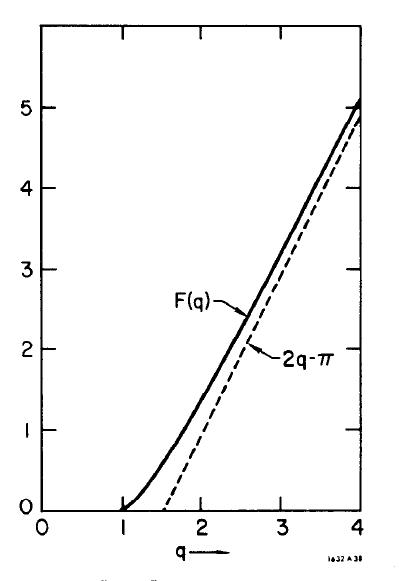
\includegraphics[width=0.5\linewidth]{./Figuras/fig38.jpeg}
	\caption{Função da abertura dinâmica $F(q)$.}
	\label{fig:fig38}
\end{figure}

Finalmente, pensando no que acontece se um elétron inicia fora da abertura dinâmica --  diga-se em pontos acima do ponto D na curva de $\Phi(\tau)$ na \autoref{fig:fig36}(b) -- e descobrindo qual seria sua trajetória de fase, o resultado seriam as curvas da \autoref{fig:fig39}. três separatrizes sucessivas são mostradas e diversos exemplos de trajetórias instáveis. Novamente, observa-se que um elétron que começa sua trajetória fora de uma região estável irá -- exceto por um fortuno acidente -- ficar fora para sempre.

\begin{figure}[!htb]
	\centering
	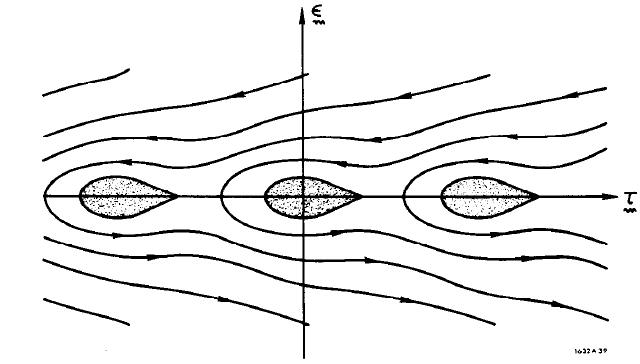
\includegraphics[width=0.7\linewidth]{./Figuras/fig39.jpeg}
	\caption{Trajetórias de fase para elétrons não capturados em um \textit{bunch} (um desenho qualitativo).}
	\label{fig:fig39}
\end{figure}
	\pagebreak

\section[Amortecimento por Radiação]{Amortecimento por Radiação\footnote{Neste capítulo, assume-se que a teoria clássica sobre radiaçao eletromagnética por elétrons relativísticos já é conhecida. Desta forma, apenas uma revisão é feita, pontuando os resultados necessários para este estudo.}}\label{part4}
	\subsection{Perda de energia}\label{sec:4.1}
Um elétron relativístico acelerado em um campo macroscópico irá radiar energia eletromagnética numa taxa proporcional ao quadrado da força de aceleração. Esta taxa depende do ângulo entre a força e a velocidade do elétron e é maior por um fator $\gamma^2 = (E/mc^2)^2$ quando a força é perpendicular à velocidade em comparação a quando ela é paralela à velocidade. Em um anel de armazenamento, as forças longitudinais típicas (advindas do sistema de aceleração) são muito menores que as forças transversais típicas e $\gamma^2$ é um número grande de fato, então apenas é necessário considerar os efeitos de radiação correspondentes às forças magnéticas.

Seja $P_\gamma$ a taxa de perda de energia por radiação, então pode-se escrever que
\begin{align}
	P_\gamma = \frac{2}{3}\frac{r_e c}{(mc^2)^3} E^2 F_\perp^2
\end{align}
onde $m$ é a massa de repouso do elétron, $r_e$ é o raio clássico do elétron e $F_\perp$ é a força magnética sobre o elétron. Será conveniente definir a constante
\begin{align}
	C_\gamma = \frac{4\pi}{3}\frac{r_e}{(mc^2)^3} = 8.85 \times 10^{-5}\ metro-GeV^{-3}\label{eq:4.2}
\end{align}
Pela força de Lorentz, $F_\perp = ecB$. Desta forma, a energia radiada é
\begin{align}
	P_\gamma = \frac{e^2c^3}{2\pi}C_\gamma E^2 B^2\label{eq:4.3}
\end{align}
Esta potência instantânea é proporcional ao quadrado tanto da energia quanto da força do campo magnético local. Às vezes é útil expressar  a força magnética em termos do raio de curvatura local $\rho$ da trajetória; então
\begin{align}
	P_\gamma = \frac{c\ C_\gamma}{2\pi}\frac{E^4}{\rho^2}\label{eq:4.4}
\end{align}

Um elétron circulando na órbita ideal tem energia nominal $E_0$ e se move com o raio de curvatura $\rho_s = 1/G$ -- veja a \autoref{sec:2.2}. Para encontrar a energia $U_0$ radiada em uma revolução, basta integrar $P_\gamma$ com relação ao tempo  ao longo do anel. Como $dt = ds/c$,
\begin{align}
	U_0 = \frac{C_\gamma E_0^4}{2\pi}\int\limits_{0}^{L}G^2(s)ds\label{eq:4.5}
\end{align}

Pode-se aproximar a integral pela média de $G^2$ multiplicada por $L=2\pi R$, o comprimento do anel:
\begin{align}
	U_0 = C_\gamma E_0^4 R \mean{G^2}
\end{align}
Para um campo guia isomagnético\footnote{Veja a \autoref{sec:2.2}.} $G = G_0=1/\rho_0$ em partes curvas de tamanho $2\pi\rho_0$ e zero nas demais partes, então
\begin{align}
	\mean{G^2} = \frac{G_0}{R} = \frac{1}{R \rho_0}\ \ (isomag.)
\end{align}
e
\begin{align}
	U_0 = \frac{C_\gamma E_0^4}{\rho_0}\ \ (isomag.)
\end{align}
\begin{proof}
	A aproximação feita anteriormente foi
	\begin{align*}
		\int\limits_{0}^{L}G^2(s)ds = \mean{G^2}L \therefore \mean{G^2} = \frac{1}{L}\int\limits_{0}^{L}G^2(s)ds
	\end{align*}
	Agora, para o caso isomagnético, $G=G_0=1/\rho_0$ nos ímãs de comprimento $2\pi \rho_0$ e zero no resto do anel. Logo, a integral fica
	\begin{align*}
		\int\limits_{0}^{L}G^2(s)ds = \int\limits_{0}^{2\pi\rho_0}G_0^2(s)ds &= 2\pi\rho_0\ G_0^2 = 2\pi\rho_0 \frac{1}{\rho_0^2} = 2\pi \frac{1}{\rho_0}\\
		\therefore \mean{G^2} &= \frac{2\pi}{L} \frac{1}{\rho_0} = \frac{1}{R \rho_0}
	\end{align*}
	Substituindo em $U_0$,
	\begin{align*}
		U_0 = C_\gamma E_0^4 R \mean{G^2} = C_\gamma E_0^4 R \frac{1}{R \rho_0} = \frac{C_\gamma E_0^4}{\rho_0}
	\end{align*}
	c.q.d.
\end{proof}

Para um raio fixo $\rho_0$, a energia radiada por revolução varia com a quarta potência da energia do elétron. A potência média radiada é $U_0/T_0$ onde $T_0 = c/2\pi R$ é o tempo de uma revolução. Para um campo guia qualquer
\begin{align}
	\mean{P_\gamma} = \frac{c C_\gamma}{2\pi} E_0^4 \mean{G^2}\label{eq:4.9}
\end{align} 
E para um anel isomagnético,
\begin{align}
	\mean{P_\gamma} = \frac{c C_\gamma}{2\pi}\frac{E_0^4 G_0}{R} = \frac{c C_\gamma E_0^4}{L \rho_0}\ \ (isomag.)\label{eq:4.10}
\end{align}

Um elétron que não está na órbita ideal perde energia a uma taxa diferente. Considere primeiro um elétron com energia nominal circulando com oscilações betatron. Sua taxa de radiação será diferente da de um elétron movendo-se na órbita ideal somente porque ele passa por um campo magnético ligeiramente diferente -- devido ao seu deslocamento betatron. Mas em cada azimutal seu desvio é igualmente positivo ou negativo. E foi assumido que os campos variam apenas de forma linear com o deslocamento. Então, analisando a amplitude betatron considerando termos de até primeira ordem, a potência radiada média em um ciclo betatron é a mesma de um elétron na órbita ideal.

O mesmo não é verdadeiro para um elétron com energia diferente de $E_0$. Este caso será analisado a seguir.

Para elétrons ultra-relativísticos, a radiação é emitida primitivamente na direção do movimento. A maioria da radiação é emitida com um ângulo $1/\gamma$. A força de reação da radiação -- e, portanto, a mudança de momento associada -- é exatamente na direção oposta do movimento\footnote{Desprezando efeitos quânticos. Veja a \autoref{sec:5.1}.}. O único efeito da radiação é diminuir a energia do elétron, sem mudar a direção do seu movimento.
	\subsection{Amortecimento das oscilações de energia}\label{sec:4.2}
Na \autoref{sec:3.5} foi visto que pequenas oscilações de energia eram amortecidas a uma taxa proporcional à mudança na perda por radiação com a energia. Pelas equações \eqref{eq:3.24} e \eqref{eq:3.42}, o coeficiente de amortecimento é
\begin{align}
	\alpha_\epsilon = \frac{D}{2T_0} = \frac{1}{2T_0}\left(\frac{dU_{rad}}{dE}\right)_0
\end{align}
onde $U_{rad}$ é a energia perdida por revolução. Quando a energia de um elétron varia da energia nominal $E_0$, a energia radiada em uma revolução muda em parte por causa da mudança de energia, em parte porque o elétron viaja em um campo magnético diferente, e em parte porque o tamanho da sua trajetória é diferente. Hora de analisar como $U_{rad}/dE$ deve ser avaliada.

Já foi visto que a oscilação betatron não muda, em uma análise de primeira ordem, a potência média radiada. Então, para obter $U_{rad}$ para qualquer energia, basta apenas integrar $P_\gamma$ da equação \eqref{eq:4.3} com relação ao tempo em uma órbita fechada completa. No entanto, será conveniente mudar a variável de integração para $s$. Assim,
\begin{align}
	U_{rad} = \oint P_\gamma dt = \oint P_\gamma \frac{dt}{ds}ds
\end{align}
lembrando que esta análise está sobre o comprimento da órbita fechada, o qual não é necessariamente o comprimento da órbita ideal. Pois bem, $dt/ds$ já foi avaliado anteriormente, veja equação  \eqref{eq:2.15}:
\begin{align*}
	\frac{dt}{ds} = \frac{1}{c} \left(1+\frac{x}{\rho_s}\right)
\end{align*}
onde $x$ é o deslocamento com relação à órbita ideal e $\rho_s = \rho(s)$ o raio de curvatura da órbita ideal. Como o interesse está sobre a perda de energia em uma órbita fechada, deve-se tomar $x = \eta \epsilon/E_0$, onde $\epsilon = E-E_0$ e $\eta(s)$ é a função de dispersão. Veja a equação \eqref{eq:2.28}. Logo,
\begin{align}
	U_{rad} = \frac{1}{c} \oint \left(1+ \frac{\eta}{\rho}\frac{\epsilon}{E_0}\right)P_\gamma ds
\end{align}

Esta integral já foi analisada para $\epsilon=0$; é apenas $U_0$. Então pode-se fazer diferente a analisar a derivada em $\epsilon=0$:
\begin{align}
	\frac{dU_{rad}}{dE} = \frac{1}{c} \oint \left(\frac{dP_\gamma}{dE}+ \frac{\eta}{\rho}\frac{P_\gamma}{E_0}\right)_0 ds\label{eq:4.14}
\end{align}
onde o subscrito "0" significa que todas as quantidades do integrando est]ao sendo avaliadas na órbita ideal, e na energia $E_0$. Pela equação \eqref{eq:4.3} $P_\gamma$ é porporcional ao produto $E^2B^2$ -- e lembre-se que quando $E$ muda, a órbita se move para uma posição diferente então $B$ também muda. Então pode-se escrever que
\begin{align*}
	\frac{dP_\gamma}{dE} = 2\frac{P_\gamma}{E_0} + 2\frac{P_\gamma}{B_0}\frac{dB}{dE}
\end{align*}

\begin{proof}
	$P_\gamma$ é dado por
	\begin{align*}
		P_\gamma = \frac{e^2c^3}{2\pi}C_\gamma E^2 B^2
	\end{align*}
	Logo, $dP_\gamma/dE$ é
	\begin{align*}
		\frac{dP_\gamma}{dE} = \frac{d}{dE}\left(\frac{e^2c^3}{2\pi}C_\gamma E^2 B^2\right) = \frac{e^2c^3}{2\pi}C_\gamma \frac{d}{dE}(E^2B^2)
	\end{align*}
	Derivando $B^2E^2$ com relação à energia, tem-se que
	\begin{align*}
		\frac{d}{dE}(E^2B^2) = 2EB^2\frac{dE}{dE} + 2E^2B\frac{dB}{dE} = 2EB^2 + 2E^2B\frac{dB}{dE}
	\end{align*}
	Substituindo, na expressão de $dP_\gamma/dE$:
	\begin{align*}
		\frac{dP_\gamma}{dE} = \frac{e^2c^3}{2\pi}C_\gamma \left(2EB^2 + 2E^2B\frac{dB}{dE}\right) = 2\frac{e^2c^3}{2\pi}C_\gamma E B^2 + 2\frac{e^2c^3}{2\pi}C_\gamma E^2 B \frac{dB}{dE}
	\end{align*}
	Pode-se substituir a equação de $P_\gamma$, obtendo-se
	\begin{align*}
		\frac{dP_\gamma}{dE} = 2\frac{P_\gamma}{E} + 2\frac{P_\gamma}{B}\frac{dB}{dE}
	\end{align*}
	Avaliando a expressão na órbita ideal,
	\begin{align*}
		\frac{dP_\gamma}{dE} = 2\frac{P_\gamma}{E_0} + 2\frac{P_\gamma}{B_0}\frac{dB}{dE}
	\end{align*}
\end{proof}

Mas
\begin{align*}
	\frac{dB}{dE} = \frac{dx}{dE}\frac{dB}{dx} = \frac{\eta}{E_0}\frac{dB}{dx}
\end{align*}
onde $dB/dx$ é uma propriedade do campo guia. Juntando as duas últimas equações na equação \eqref{eq:4.14}, tem-se que
\begin{align*}
	\frac{dU_{rad}}{dE} = \frac{1}{c}\oint \left(2\frac{P_\gamma}{E} + 2\frac{P_\gamma}{B}\frac{\eta}{E_0}\frac{dB}{dx} + \frac{P_\gamma}{E}\frac{\eta}{\rho}\right)_0 ds
\end{align*}

A integral do primeiro termo é apenas $2U_0/E_0$, então
\begin{align}
	\frac{dU_{rad}}{dE} = \frac{U_0}{E_0}\left[2+\frac{1}{cU_0}\oint \left(\eta P_\gamma \left[\frac{1}{\rho} + \frac{2}{B}\frac{dB}{dx}\right]\right)_0 ds\right]
\end{align}

Então pode-se escrever que a constante de amortecimento é dada por
\begin{align}
	\alpha_\epsilon = \frac{1}{2T_0}\left(\frac{dU_{rad}}{dE}\right)_0 = \frac{U_0}{2T_0E_0}(2+\mathscr{D})\label{eq:4.16}
\end{align}
com
\begin{align}
	\mathscr{D} = \frac{1}{cU_0}\oint \left[\eta P_\gamma\left(\frac{1}{\rho}+\frac{2}{B}\frac{dB}{dx}\right)\right]_0 ds\label{eq:4.17}
\end{align}
Tomando $P_\gamma$ e $U_0$ das equações \eqref{eq:4.3} e \eqref{eq:4.5} e expressando $B$ e $dB/dx$ em termos de $G(s)$ e $K_1(s)$ assim como foram definidos na \autoref{sec:2.2}, $\mathscr{D}$ pode ser reescrito como
\begin{align}
	\mathscr{D} = \frac{\oint \eta G \left(G^2 + 2K_1\right)ds}{\oint G^2 ds}\label{eq:4.18}
\end{align}

\begin{proof}
	Pelas equações \eqref{eq:4.3} e \eqref{eq:4.5}, tem-se que
	\begin{align*}
		P_\gamma = \frac{e^2c^3}{2\pi}C_\gamma E^2B^2\\
		U_0 = \frac{C_\gamma E_0^4}{2\pi}\oint G^2 ds
	\end{align*}
	Substituindo na equação \eqref{eq:4.17}:
	\begin{align*}
		\mathscr{D} &= \frac{2\pi}{c C_\gamma E_0^4}\frac{1}{\oint G^2 ds}\oint \left[\eta \frac{e^2c^3}{2\pi}C_\gamma E^2B^2 \left(\frac{1}{\rho}+\frac{2}{B}\frac{dB}{dx}\right)\right]_0 ds\\
					&= \frac{\oint \left[\eta \frac{e^2c^2}{E_0^2} B^2 \left(\frac{1}{\rho}+\frac{2}{B}\frac{dB}{dx}\right)\right]_0 ds}{\oint G^2 ds}
	\end{align*}
	Agora, recuperando os valores de $G(s)$ e $K_1(s)$ da \autoref{sec:2.2}, pode-se substituí-los e obter
	\begin{align*}
		\mathscr{D} &= \frac{\oint \left[\eta G^2 \left(G +\frac{2ec}{G E_0}\frac{K_1 E_0}{ec}\right)\right]_0 ds}{\oint G^2 ds}\\
					&= \frac{\oint \left[\eta G^2 \left(G +\frac{2K_1}{G}\right)\right]_0 ds}{\oint G^2 ds}\\
		\therefore \mathscr{D} &= \frac{\oint \left[\eta G \left(G^2 +2K_1\right)\right]_0 ds}{\oint G^2 ds}
	\end{align*}
	c.q.d.
\end{proof}

Essa forma torna claro o fato de que $\mathscr{D}$ é um número o qual é uma propriedade da configuração total do campo guia -- obtido da integração ao redor do anel das expressões envolvendo apenas as funções do campo guia $G$, $K_1$ e $\eta$. O número $\mathscr{D}$ tipicamente é positivo e um pouco maior que 1.

A equação \eqref{eq:4.16} tem uma interpretação física relevante. Já que $\mathscr{D}$ é tipicamente pequeno, pode-se aproximar a relação
\begin{align}
	\alpha_\epsilon \approx \frac{U_0}{E_0T_0} = \frac{\mean{P_\gamma}}{E_0}\label{eq:4.20}
\end{align}
onde $\mean{P_\gamma}$ é a taxa média de perda de radiação. A constante de tempo de amortecimento para oscilações de energia -- a qual é o inverso de $\alpha_\epsilon$ -- é apenas o tempo necessário para um elétron radiar toda a sua energia!

A expressão de $\mathscr{D}$ se torna mais simples para um campo guia isomagnético. Neste caso, $G(s)$ é zero ou um valor constante $G_0$ nos ímãs, então as integrais são avaliadas apenas nos ímãs. A equação \eqref{eq:4.18} torna-se
\begin{align}
	\mathscr{D} = \frac{1}{2\pi} \int\limits_{mag}^{}\eta(s)\left[G_0^2 + 2K_1(s)\right]ds\ \ (isomag)
\end{align}

\begin{proof}
	Como já foi dito, $G(s)$ é zero ou um valor constante $G_0$ nos ímãs, então as integrais são avaliadas apenas nos ímãs. Logo, $\mathscr{D}$ torna-se
	\begin{align*}
		\mathscr{D} &= \frac{\int\limits_{mag}^{} \eta G_0 \left(G_0^2 + 2K_1\right)ds}{\int\limits_{mag}^{} G_0^2 ds} = \frac{G_0\int\limits_{mag}^{} \eta \left(G_0^2 + 2K_1\right)ds}{2\pi \rho_0 G_0^2}\\
		 &= \frac{1}{2\pi \rho_0 G_0}\int\limits_{mag}^{} \eta \left(G_0^2 + 2K_1\right)ds
	\end{align*}
	Mas $G_0 = 1/\rho_0$. Então,
	\begin{align*}
		\mathscr{D} = \frac{1}{2\pi}\int\limits_{mag}^{} \eta \left(G_0^2 + 2K_1\right)ds
	\end{align*}
\end{proof}

Se o campo guia também é de função separável, os ímãs não possuem gradiente de campo e
\begin{align}
	\mathscr{D} = \frac{G_0^2}{2\pi}\int\limits_{mag}^{}\eta(s)ds\ \ (isomag.\ e\ fun. sep.)
\end{align}
esta integral é familiar: ela apareceu anteriormente quando o fator de compactação de momento $\alpha$ foi calculado para um campo guia isomagnético. Utilizando as equações \eqref{eq:3.13} e \eqref{eq:3.14}:
\begin{align}
	\mathscr{D} = G_0\mean{\eta}_{mag} = G_0\alpha R = \frac{\alpha R}{\rho_0}\ \ (isomag.\ e\ fun. sep.)
\end{align}
Para este tipo de anel, o número $\mathscr{D}$ é apenas o fator de compactação de momento aumentado por uma razão entre o raio de curvatura típico $R$ e o raio de curvatura do ímã $\rho_0$. Alguns valores típicos para estes parâmetros:
\begin{align}
	\alpha \approx 0.05;\ \ \ R/\rho_0 \approx 3;\ \ \ \mathscr{D} \approx 0.15.
\end{align}
Recapitulando, para oscilações de energia em um campo guia isomagnético e de função separável, o coeficiente de amortecimento por oscilações de energia é
\begin{align}
	\alpha_\epsilon = \frac{\mean{P_\gamma}}{2E_0}\left(2+ \frac{\alpha R}{\rho_0}\right)\ \ (isomag.\ e\ fun. sep.)
\end{align}
	\subsection{Amortecimento das oscilações betatron}\label{sec:4.3}
Já é hora de analisar o amortecimento por radiação das oscilações betatron. Aqui será dado apenas um tratamento aproximado, porém por meio de um método que -- com apenas um pouco de álgebra -- pode ser estendido a um cálculo exato. De qualquer forma, o resultado exato é mais facilmente obtido por um teorema geral que será discutido na \autoref{sec:4.4}.

Começando pelas oscilações betatron verticais (a notação será a mesma usada na \autoref{part2}). O movimento será aproximado ignorando a variação de $\beta$ com $s$, então pode-se escrever (veja a \autoref{sec:2.8}):
\begin{align}
	z = A\ cos(\varphi), \ \ z' = \frac{A}{\beta}\ sen(\varphi)\label{eq:4.24}
\end{align}
onde $\varphi = s/\beta$. A amplitude de oscilação $A$ pode ser obtida por $z$ e $z'$ em qualquer instante por
\begin{align}
	A^2 = z^2 + (\beta z')^2
\end{align}
Suponha um elétron com energia nominal $E_0$ -- o qual está oscilando verticalmente sobre a órbita ideal. Em qualquer elemento azimutal $\delta s$ o elétron irá perder por radiação uma pequena quantidade de energia $\delta E$. Seu vetor de momento $p$ será mudado por $\delta p$ e, como foi apontado anteriormente, $\delta p$ é paralelo (e oposto) a $p$, então $|\delta p| = \delta E/c$. Veja a \autoref{fig:fig40}(a). A perda por radiação não muda nem o desvio nem a inclinação da trajetória (as variações de $z$ e de $s$ com relação ao tempo existem, mas compensam uma a outra); então a amplitude $A$ não é alterada pela radiação. Existe um pequeno efeito causado pelas forças focalizadoras efetivas e, portanto, $\beta$ também varia com uma mudança na energia. Este efeito é chamado de amortecimento adiabático, porém é um efeito de segunda ordem e pode ser ignorado nesta análise já que a energia não varia na média quando a aceleração de RF é considerada.

\begin{figure}[!htb]
	\centering
	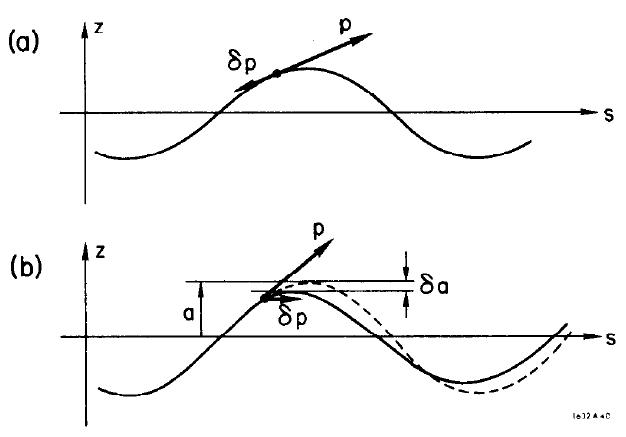
\includegraphics[width=0.7\linewidth]{./Figuras/fig40.jpeg}
	\caption{Efeito da mudança de energia nas oscilações betatron verticais: (a) por perda por radiação, (b) por aceleração de RF. Retirado de \cite{sands1970physics}.}
	\label{fig:fig40}
\end{figure}

Agora, note que o efeito da força de aceleração de RF é um pouco diferente. Esta força é, na média, paralela à órbita ideal. Então o incremento de momento $\delta p$ recebido no elemento azimutal $\delta s$ não é mais exatamente paralelo a $p$. Veja a \autoref{fig:fig40}(b). Seja $p_\perp$ a componente  de $p$ perpendicular à órbita ideal; então, como os ângulos são pequenos, pode-se aproximar
\begin{align*}
	z' = \frac{p_\perp}{p}
\end{align*}
Novamente, a força de aceleração não muda $z$. Mas, de fato, muda $z'$ que, considerando apenas termos lineares, vai para
\begin{align}
	z' \rightarrow \frac{p_\perp}{p+\delta p} = \frac{p_\perp}{p}\left(1-\frac{\delta p}{p}\right) = z'\left(1-\frac{\delta p}{p}\right)
\end{align}
Assim, mudança em $z'$ é
\begin{align}
	\delta z' = -z'\frac{\delta p}{p} = -z'\frac{\delta E}{E}
\end{align}
Existe uma mudança correspondente na amplitude $A$;
\begin{align}
	A\delta A = \beta^2 z' \delta z' = -(\beta z')^2 \frac{\delta E}{E}
\end{align}

\begin{proof}
	Considerando que o movimento vertical é dado pela equação \eqref{eq:4.24}, então, considerando variações $z'$ e $A$, tem-se que
	\begin{align*}
		z = (A+\delta A)\ cos(\varphi), \ \ (z' + \delta z') = \frac{(A+\delta A)}{\beta}\ sen(\varphi)
	\end{align*}
	Logo, por relação trigonométrica, obtém-se que
	\begin{align*}
		(A+\delta A)^2 &= z^2 + (\beta (z'+\delta z'))^2\\
		A^2+2 A \delta A + \delta A^2 &= z^2 + \beta^2 (z'^2 + 2z'\delta z' + \delta z'^2)
	\end{align*}
	Descartando os temos de segunda ordem:
	\begin{align*}
		2 A \delta A &= \beta^2 2z'\delta z'\\
		\therefore A\delta A &= \beta^2 z' \delta z'
	\end{align*}
	c.q.d.
\end{proof}

Agora, a fase de oscilação na chegada do elétron no ponto $s$ é arbitrária (e todos os valores entre $0$ e $2\pi$ são igualmente prováveis) então apenas a mudança média em $A$ importa. A média de $(z'^2)$ é $A^2/2\beta^2$, então
\begin{align}
	A\mean{\delta A} = -\frac{A^2}{2}\frac{\delta E}{E_0}
\end{align}

Suponha que todos os elementos do ganho de aceleração sejam somados em uma revolução. Como a soma de todos os $\delta E$ deve resultar em $U_0$, obtém-se que a mudança $\Delta A$ que ocorre em $A$ em uma revolução (devido à aceleração de RF) é
\begin{align}
	\frac{\Delta A}{A} = -\frac{U_0}{2E_0}\label{eq:4.30}
\end{align}
Como $\Delta A$ em cada período de revolução $T_0$ é proporcional a $A$, o movimento é amortecido exponencialmente -- como $e^{-\alpha_z t}$. Ou seja,
\begin{align}
	\frac{1}{A}\frac{dA}{dt} = \frac{\Delta A}{A T_0} = -\frac{U_0}{2E_0T_0}
\end{align}
então o coeficiente de amortecimento é
\begin{align}
	\alpha_z = \frac{U_0}{2E_0T_0} = \frac{\mean{P_\gamma}}{2E_0}
\end{align}
Pode-se mostrar que um cálculo exato -- usando a forma completa das oscilações betatron verticais -- leva ao mesmo resultado. Note que a taxa de amortecimento das oscilações verticais é apenas $1/2$ da taxa típica das oscilações de energia (quando $\mathscr{D}$ é pequeno); veja a equação \eqref{eq:4.20}.

É muito importante notar que o amortecimento "por radiação" não ocorre no processo de perda por radiação, mas sim no processo de ganho de energia do sistema de RF. Isto poderia ser um motivo de questionamento sobre o nome "amortecimento por radiação". Mas, pensando bem, não existiria oportunidade para amortecimento pelos campos de RF se não fosse necessário compensar a perda de energia por radiação. Então o nome "amortecimento por radiação" não é tão ruim.

Agora, hora de analisar os efeitos da radiação sobre as oscilações betatron radiais. Num primeiro momento, pode-se pensar que as oscilações betatron radiais deveriam ser amortecidas do mesmo modo que as verticais. Porém existem complicações adicionais que fazem com que este problema deva ser tratado separadamente. Um novo elemento aparece devido à mudança do deslocamento betatron que ocorre quando existe uma mudança na energia. Lembre-se que o deslocamento radial total $x$ é a soma de duas partes: o deslocamento $x_\epsilon$ da órbita fechada e o deslocamento beatron $x_\beta$ com relação a esta órbita,
\begin{align}
	x = x_\epsilon + x_\beta\label{eq:4.33}
\end{align}

Quando a energia de um elétron muda por uma quantidade $\delta E$, existe uma mudança em $x_\epsilon$ pela quantidade, veja a equação \eqref{eq:2.28},
\begin{align}
	\delta x_\epsilon = \eta \frac{\delta E}{E_0}
\end{align}
Mas, como a posição do elétron no espaço não muda por um impulso momentâneo finito, o deslocamento total $x$ não muda, então obrigatoriamente existe uma compensação em $x_\beta$. Isto é, da equação \eqref{eq:4.33},
\begin{align*}
	\delta x = \delta x_\epsilon + \delta x_\beta = 0
\end{align*}
de forma que
\begin{align}
	\delta x_\beta = -\delta x_\epsilon = -\eta \frac{\delta E}{E_0}\label{eq:4.35}
\end{align}
Quando ocorre uma variação na energia, o elétron não se move instantaneamente, mas o eixo de referência das suas oscilações sim e o deslocamento com respeito a este eixo é, portanto, alterado --  como é ilustrado na \autoref{fig:fig41}.

\begin{figure}[!htb]
	\centering
	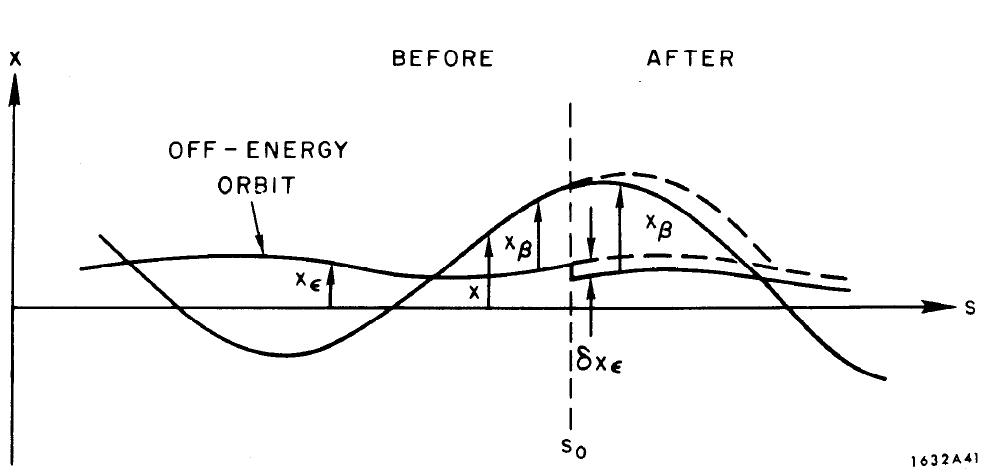
\includegraphics[width=0.9\linewidth]{./Figuras/fig41.jpeg}
	\caption{Efeito de uma mudança repentina de energia em $s_0$ sobre o deslocamento betatron radial. Retirado de \cite{sands1970physics}.}
	\label{fig:fig41}
\end{figure}

Algo similar ocorre na inclinação betatron. Correspondendo à equação \eqref{eq:4.33}, tem-se
\begin{align}
	x' = x'_\epsilon + x'_\beta
\end{align}

Agora, porém, um impulso elementar pode mudar a inclinação total $x'$ por algum $\delta x'$, então deve-se ter
\begin{align}
	\delta x'_\beta = \delta x' - \delta x'_\epsilon
\end{align}
Tomando a derivada de $x_\epsilon$ da equação \eqref{eq:2.28},
\begin{align}
	\delta x'_\beta = \delta x' - \eta' \frac{\delta E}{E_0}\label{eq:4.38}
\end{align}
onde $\eta'$ é, claro, $d\eta/ds$. Mesmo que $\delta x'$ seja zero, uma mudança na inclinação de $x_\epsilon$ -- o eixo de referência da oscilação -- produziria uma mudança na inclinação da oscilação betatron.

Existe mais uma complicação adicional devido à curvatura da órbita de referência. As metades positiva e negativa de uma oscilação betatron ocorrem em intervalos iguais de $s$, mas o elétron viaja um comprimento de caminho maior na parte positiva do que na negativa --  veja a equação \eqref{eq:3.7}. Apesar do efeito total sobre o comprimento de caminho ser nulo em uma revolução completa, existe, em geral, uma diferença na quantidade de energia perdida por radiação durante as duas metades da oscilação. E a amplitude da oscilação é, logo, afetada.

Aplicando, agora, estas ideias sobre a perda por radiação $\delta E$ em um elemento azimutal $\delta s$. Um cálculo preciso pode ser feito a partir das mudanças em $x$ e $x'$ obtidas nas equações \eqref{eq:4.35} e \eqref{eq:4.38}. Porém, mantendo as aproximações feitas anteriormente, pode-se fazer uma suposição simplificada de que $\eta$ é uma constante, então $\eta'=0$; e escrever a variação de $x_\beta$ com $s$ na mesma forma que a variação betatron vertical, ou seja,
\begin{align}
	x_\beta = A\ cos(\varphi), \ \ x'_\beta = \frac{A}{\beta}\ sen(\varphi)
\end{align}
Desta vez, tem-se que
\begin{align}
	A \delta A = x_\beta \delta x_\beta + \beta^2 x'_\beta \delta x'_\beta
\end{align}
Pela suposição de que $\eta$ é constante, $x'_\epsilon = 0$. Logo, $x' = x'_\beta$ e $\delta x' = \delta x'_\beta$, então uma mudança de energia não causa variação na inclinação. Logo, $\delta x_\beta = 0$ e
\begin{align}
	A \delta A = -x_\beta \eta \frac{\delta E}{E_0}\label{eq:4.41}
\end{align}

Novamente, toma-se o desvio de energia $\delta E$ como a perda por radiação em um elemento azimutal $\delta s$. Para o movimento vertical, assumiu-se que o elétron estava sempre se movendo com deslocamento radial nulo, então a taxa de perda por radiação era a mesma (até termos de primeira ordem em $x$) que a taxa de perda de energia na órbita ideal. Já para o movimento radial, se os ímãs possuem gradiente de campo, as coisas são um pouco diferentes. Para simplificar a discussão, a análise será sobre um campo guia isomagnético de função separável. Em uma máquina com função separável, a taxa de perda por radiação independe de $x$ -- até termos de primeira ordem.\footnote{Há apenas gradiente de campo nos quadrupolos; onde $B$ é proporcional a $x$. Como a taxa de radiação varia com $B^2$, não há efeito de primeira ordem.}Desta forma, pode-se considerar que, para um elétron com energia nominal, a taxa de perda por radiação $P_\gamma(s)$ não depende de $x$, apenas de $s$. Então, a variação de energia em um elemento de caminho $\Delta \ell$ é
\begin{align}
	\delta E = -\frac{P_\gamma}{c}\Delta \ell
\end{align}

Tomando $\Delta \ell$ da expressão em \eqref{eq:2.15},
\begin{align}
	\delta E = -\left(1+\frac{x_\beta}{\rho_s}\right)\frac{P_\gamma}{c}\Delta s
\end{align}

Combinando este resultado com a equação \eqref{eq:4.41}, tem-se que a mudança de amplitude é
\begin{align}
	A \delta A = x_\beta \eta \left(1+\frac{x_\beta}{\rho_s}\right)\frac{P_\gamma}{cE_0}\Delta s
\end{align}
Novamente, apenas o valor esperado de $\delta A$ é importante -- a média sobre todos os ângulos de fase $\varphi$. O valor esperado de $x_\beta$ é zero e de $x_\beta^2$ é $A^2/2$; então tem-se que
\begin{align}
	\frac{\mean{\delta A}}{A} = \frac{\eta}{2 \rho_s}\frac{P_\gamma}{cE_0}\Delta s
\end{align}

Como foi assumido um campo guia isomagnético, em qualquer lugar que $P_\gamma$ for diferente de 0, $\rho = \rho_s = 1/G_0$ e pode-se somar o efeito em cada $\Delta s$ para obter a variação $\Delta A$ em uma revolução completa. A soma de todos os termos $P_\gamma s/c$ é apenas a perda de energia $U_0$ em uma volta completa. Então o efeito da radiação é
\begin{align}
	\left(\frac{\Delta A}{A}\right)_{rad} = \frac{\eta}{2 \rho_0}\frac{U_0}{E_0}
\end{align}
Observe que o sinal do lado direito da equação é positivo. Ou seja, há um aumento da amplitude devido à radiação!

Felizmente, esta é apenas uma parte da análise. Também é preciso considerar o efeito da aceleração de RF. Porém, existe um efeito de "tamanho de caminho" correspondente. Geralmente, as cavidades de RF são localizadas onde $\rho = \infty$, ou seja, em trechos retos. Mas, de qualquer forma, é uma propriedade destas cavidades que o ganho de energia seja (até primeira ordem, ao menos) independente do deslocamento betatron. O cálculo da contribuição da aceleração de RF ocorre da mesma forma que no movimento vertical, com o resultado da equação \eqref{eq:4.30}. Para obter o efeito total em uma revolução é preciso computar as contribuições da perda por radiação e da aceleração para obter
\begin{align}
	\frac{\Delta A}{A} = -\left(1-\frac{\eta}{\rho_0}\right)\frac{U_0}{2E_0}
\end{align}
o que gera o coeficiente de amortecimento $\alpha_x$ das oscilações radiais
\begin{align}
	\alpha_x = \left(1-\frac{\eta}{\rho_0}\right)\frac{U_0}{2E_0T_0}\label{eq:4.48}
\end{align}
Um cálculo preciso para um campo guia isomagnético de função separável chega neste mesmo resultado se $\eta$ por substituído por $\mean{\eta}_{mag}$, o valor médio de $\eta(s)$ no ímãs. Mas retomando a equação \eqref{eq:3.14}, $\mean{\eta}_{mag} = \alpha R$ então
\begin{align}
	\alpha_x = \left(1-\frac{\alpha R}{\rho_0}\right)\frac{U_0}{2E_0T_0}\ \ (isomag.\ e\ fun. sep.)\label{eq:4.49}
\end{align}

Considerando que $\alpha R/\rho_0$ é menor que 1 -- como este termo usualmente é -- o coeficiente de amortecimento é positivo e as oscilações radiais são amortecidas. Mas existe um efeito "anti-amortecimento" da radiação -- o termo $\alpha R/\rho_0$ -- que vai contra o amortecimento positivo do sistema. Enquanto o termo anti-amortecimento for pequeno, este não causa problema algum.

Comparando a equação \eqref{eq:3.49} com os resultados da \autoref{sec:4.2} é possível observar que o resultado também pode ser escrito em termos de $\mathscr{D}$\footnote{Este resultado é obtido mudando um pouco as aproximações feitas: ao invés de considerar que há um $\delta x'$ e considerar $\eta$ constante, considere que $\delta x'=0$ e considere a variação de $\eta$ com $s$.}:
\begin{align}
	\alpha_x = (1-\mathscr{D})\frac{U_0}{2E_0T_0}\ \ (geral)\label{eq:4.50}
\end{align}
Apesar deste resultado ter sido obtido apenas para um tipo específico de campo guia (e com algumas aproximações), a equação \eqref{eq:4.50} é exata para qualquer campo guia. Isto é, se a variação de $\eta$ com $s$ tivesse sido considerada, no lugar do termo $\eta/\rho_0$ na equação \eqref{eq:4.48} haveria a expressão completa de $\mathscr{D}$ da equação \eqref{eq:4.17}. Mais será dito a seguir sobre esta interessante "coincidência".
	\subsection{Taxas de amortecimento por radiação}\label{sec:4.4}
Efeitos de amortecimento por radiação já foram considerados sobre os três graus de liberdade de um elétron em um \textit{bunch}: os dois deslocamentos betatron transversais $x_\beta$ e $z_\beta$ e as oscilações de energia -- as quais apareceram associadas às oscilações de $\tau$ e $x_\epsilon$. Cada um dos três modos de oscilação possui um decaimento exponencial natural com coeficientes de amortecimento $\alpha_i$ (com $i=x,z,\epsilon$) que podem ser convenientemente expressados como
\begin{align}
	\alpha_i = J_i \alpha_0 = J_i\frac{\mean{P_\gamma}}{2E_0}
\end{align}
com
\begin{align}
	J_x=1-\mathscr{D}\ \ \ \ \ J_z=1\ \ \ \ \ J_\epsilon=2+\mathscr{D}\label{eq:4.52}
\end{align}
As constantes de tempo de amortecimento são apenas $1/\alpha_i$, então
\begin{align}
	\tau_i = \frac{2E_0}{J_i \mean{P_\gamma}}\label{eq:4.53}
\end{align}

Para um anel de armazenamento isomagnético, $\mean{P_\gamma}$ pode ser dado pela equação \eqref{eq:4.10} e $\tau_i$ dado por
\begin{align}
	\tau_i = \frac{4\pi}{C_\gamma}\frac{R\rho_0}{J_i E_0^3}\ \ (isomag.)
\end{align}
onde $C_\gamma$ é a constante definida na equação \eqref{eq:4.2}. Neste tipo de máquina, as constantes de tempo de amortecimento variam com o inverso do cubo da energia.

O número $\mathscr{D}$ é uma propriedade do campo guia e pode ser avaliado por uma das equações \eqref{eq:4.17}, \eqref{eq:4.20} ou \eqref{eq:4.22}. Os números $J_i$ são conhecidos como números de partição de radiação já que sua soma é uma constante:
\begin{align}
	\sum J_i = J_x + J_z + J_\epsilon = 4\label{eq:4.55}
\end{align}

Apesar deste último resultado não ter sido provado de forma rigorosa, ele vem do cálculo detalhado para um campo guia qualquer. Estes cálculos não são, porém, necessários pois o Teorema de Robinson prova, em termos bem generalistas, que o teorema da equação \eqref{eq:4.55} é verdadeiro. O teorema pede apenas que todos os campos agindo sobre a partícula sejam determinados a priori e não sejam influenciados pelo movimento do elétron. Estas condições são verdadeiras se apenas os ímãs e campos de RF prescritos do anel forem considerados.

As taxas de amortecimento para apenas um elétron -- e, mais importante, para um movimento coerente de um pequeno conjunto deste -- podem ser modificadas pelos números em questão se forças adicionais que dependam de detalhes do movimento do elétron forem introduzidas. Estas forças podem, por exemplo, vir de correntes imaginárias na parede da câmara de vácuo, ou de correntes induzidas pelo elétron nas cavidades de RF, ou de forças de sistemas auxiliares de eletrodos alimentados por amplificadores de detetores  que medem o deslocamento dos elétrons. Em anéis de armazenamento reais, o primeiro efeito levou a oscilações transversais coerentes instáveis e o último geralmente as atenua. O segundo efeito tem sido tanto a causa quanto a cura de oscilações longitudinais instáveis de um \textit{bunch}. Já que estes efeitos precisam da cooperação coerente de muitos elétrons, eles estão além do escopo desta análise e não serão considerados.

Da equação \eqref{eq:4.55} também pode-se obter o resultado mais particular onde $J_x + J_\epsilon=3$. Porém, este resultado depende de uma suposição restritiva -- que a órbita ideal esteja no plano e que os campos magnéticos sejam simétricos com relação a este plano. Já foi discutida brevemente (no fim da \autoref{sec:3.1}) uma das consequências de desconsiderar esta suposição. Órbitas fechadas podem ter deslocamentos "verticais" $z_\epsilon$, da mesma forma que possuem deslocamentos "radiais" $x_\epsilon$. Isto complicaria os cálculos feitos aqui. Em particular, os números de partição não seriam dados pela equação \eqref{eq:4.52}. Porém, o teorema de "conservação" da equação \eqref{eq:4.55} iria continuar válido.

Dois outros pontos sobre a consequência deste teorema também são importantes. Primeiro, para campos guia com "gradientes alternados" -- tipo que é universal em síncrotrons e na maioria dos síncrotrons de prótons -- o número $\mathscr{D}$ é maior que 1. Como consequência, as oscilações betatron radiais são anti-amortecidas -- e crescem exponencialmente com o tempo em uma energia fixa. Este efeito não é muito grave em síncrotrons pois o aumento de amplitude causado pelo anti-amortecimento é pequeno em um tempo de aceleração. No entanto causou, em especial, problemas durante o comissionamento do síncrotron CEA. Foi necessário instalar ímãs especiais projetados para alterar $\mathscr{D}$ sem afetar significantemente as outras características do anel.

Finalmente, vale ressaltar que nenhum campo real irá satisfazer de forma exata a simetria imposta dos campos com relação ao plano da órbita ideal. As assimetrias acidentais geralmente são pequenas, mas elas irão, em geral, causar pequenos acoplamentos entre as oscilações betatron horizontal e radial. Quando este acoplamento é considerado, $x$ e $z$ não são mais as coordenadas dos modos normais. E os novos modos normais irão ter coeficientes de amortecimento que são de alguma forma diferentes de $\alpha_x$ e $\alpha_z$.
	\pagebreak

\section{Excitação por Radiação}
	\subsection{Radiação quântica}\label{sec:5.1}
Até agora apenas foi considerada a perda total de energia por radiação síncrotron -- assumindo implicitamente que esta perda de energia é um processo contínuo. Esta análise é satisfatória para uma primeira aproximação já que, na média, a perda de energia é, de fato, suave. Mas já se sabe que toda radiação eletromagnética ocorre em quantidades de energia discreta. E esta discretização da perda de energia impacta significantemente o comportamento dos elétrons no anel de armazenamento.

Cada vez que uma emissão quântica ocorre, a energia do elétron faz um pulo descontínuo. Como será visto depois, as quantidades mais significantes possuem energia em uma faixa desde a luz visível até raio-X mole. Embora tentar explicar quantitativamente os efeitos quânticos pela teoria clássica seja um terreno movediço, as afirmações quase clássicas a seguir podem ser rigorosamente justificadas. Primeiro, o "tempo" durante uma emissão quântica típica não é maior que $\rho/\gamma c$, onde $\rho$ é o raio de curvatura da trajetória e $\gamma$ a energia do elétron em termos da sua energia de repouso. Já que este tempo é muito menor que qualquer outro tempo relevante -- tal como o período de uma oscilação betatron ou de uma oscilação síncroton -- pode-se considerar que esta emissão é instantânea. Segundo, o tempo de cada emissão quântica é estatisticamente independente. Como a mudança de energia em qualquer emissão é uma fração muito pequena da energia do elétron, pode-se considerar que sucessivas emissões são processos puramente randômicos (isto é, com distribuição Poisson).

A mudança descontínua de energia advinda da emissão quântica perturba a trajetória do elétron. O efeito cumulativo de várias perturbações introduzem um tipo de "ruído" nos vários modos de oscilação, fazendo com que suas amplitudes aumentem até que, na média, a excitação quântica seja balanceada pelo amortecimento das oscilações. Este processo será detalhado posteriormente tanto para as oscilações betatron quanto para as oscilações de energia.

Talvez seja necessária aqui uma observação sobre o amortecimento. Nas seções anteriores, os efeitos de amortecimento foram relacionados à radiação. Porém, deve-se notar que o amortecimento depende apenas da taxa média de emissão de energia, e não das suas propriedades estatísticas. Então, ao considerar os efeitos quânticos, deve-se tomar o amortecimento já encontrado -- compreendendo que este ocorre devido à taxa média da perda de energia em todas as energia quânticas. Os efeitos da excitação serão causados pelas flutuações da radiação em torno da sua taxa média (Pode-se, claro, tratar ambos os efeitos da média e da flutuação juntos, porém isto apenas traria complicações indesejadas).

Ao considerar os efeitos das flutuações da radiação nas oscilações de um elétron no anel de armazenamento, deve-se saber certas propriedades sobre radiação quantificada. Então agora estas propriedades serão analisadas.

Do ponto de vista clássico, a radiação síncrona é emitida com um espectro de frequência contínuo. Considere a radiação emitida por um elétron em um intervalo finito de tempo $\Delta t$. Suponha que seja examinado o campo de radiação correspondente -- por um atraso de tempo adequado-- à emissão em $\Delta t$ e, para cada direção no espaço, seja feita uma análise de Fourier deste campo de radiação. O espectro de frequência irá, em geral, ser diferente em cada direção. Mas pode-se tomar a média do espectro em todas as direções a fim de definir o espectro de potência radiada $\mathscr{P}(\omega)$ tal que $\mathscr{P}(\omega)d\omega \Delta t$ seja a energia radiada em $\Delta t$ com frequências angulares entre $\omega e \omega+d\omega$. Claramente, a definição só faz sentido se $\Delta t$ é suficientemente grande de forma que a maioria da energia seja encontrada em frequências maiores que $1/\Delta t$. Relembre que a radiação é tipicamente emitida com um ângulo $1/\gamma$ do vetor de velocidade do elétron. Tal ângulo é varrido para fora no tempo $\rho/\gamma c$, onde $\rho$ é o raio de curvatura local da trajetória. Então um intervalo de tempo $\approx \rho/\gamma c$ deve contar a maioria do impulso de radiação; e, portanto, deve representar uma magnitude adequada para $\Delta t$. Posteriormente será visto que esta ordem de magnitude, de fato, é apropriada.

Com a definição de $\mathscr{P}(\omega)$ dada anteriormente, pode-se permitir que esta seja uma função que varia lentamente com o tempo e, por este fato, não é difícil afirmar que $\mathscr{P}(\omega)$ (e, portanto, suas variáveis de dependência $\rho$ ou $\gamma$) não variam de forma significante em $\Delta t$. Esta condição geralmente é satisfeita\footnote{Os resultados importantes desta parte requerem, na verdade, apenas que $\rho$ e $\gamma$ não mudem significantemente em um tempo $\rho/\gamma^3$, o qual é muito menor que $\Delta t$.} em anéis de armazenamento, então pode-se considerar que $\mathscr{P}(\omega)$ é o espectro de potência "instantâneo" o qual sua integral em $\omega$ é a potência radiada instantânea definida anteriormente,
\begin{align}
	P_\gamma = \int\limits_{0}^{\infty}\mathscr{P}(\omega)\ d\omega
\end{align}

O espectro de potência pode ser escrito num formato mais conveniente:
\begin{align}
	\mathscr{P}(\omega) = \frac{P_\gamma}{\omega_c} S\left(\frac{\omega}{\omega_c}\right)\label{eq:5.2}
\end{align}
com $\omega_c$ a constante definida por
\begin{align}
	\omega_c = \frac{3}{2}\frac{c\gamma^3}{|\rho|}
\end{align}
O número $\omega_c$ é chamado de frequência crítica\footnote{Cuidado! Alguns autores definem a frequência crítica com um fator numérico diferente.}, e note que é aproximadamente igual a $\gamma^3$ vezes a frequência angular de revolução do elétron. A função espectral $S(\omega/\omega_c)$ é uma função puramente algébrica, podendo ser expressada por
\begin{align}
	S(\xi) = \frac{9\sqrt{3}}{8\pi}\xi\int\limits_{\xi}^{\infty}K_{5/3}(\bar{\xi})d\bar{\xi}
\end{align}
onde $K_{5/3}$ é a função de Bessel modificada. Da definição da equação \eqref{eq:5.2}, segue que $S$ é normalizada, então
\begin{align}
	\int\limits_{0}^{\infty}S(\xi)d\xi = 1
\end{align}

\begin{proof}
	Pela definição dada na equação \eqref{eq:5.2}, tem-se que
	\begin{align*}
		P_\gamma = \int\limits_{0}^{\infty}\frac{P_\gamma}{\omega_c} S\left(\frac{\omega}{\omega_c}\right)\ d\omega\\
		\therefore \int\limits_{0}^{\infty}\frac{1}{\omega_c} S\left(\frac{\omega}{\omega_c}\right)\ d\omega = 1
	\end{align*}
	Fazendo uma mudança de variável $\xi = \omega/\omega_c $, tem-se que $d\xi = d\omega/\omega_c$. Logo,
	\begin{align*}
		\int\limits_{0}^{\infty}S(\xi)d\xi = 1
	\end{align*}
\end{proof}

A forma da função de espectro é mostrada na \autoref{fig:fig42}. Seu comportamento para grandes e pequenos argumentos -- o qual pode ser facilmente obtido a partir do comportamento assintótico da função de Bessel -- é útil, às vezes.
\begin{align}
	Para\ \xi<<1;&\ \ \ \ \ S(\xi)\approx 1.34 \xi^{1/3}\nonumber\\
	Para\ \xi>>1;&\ \ \ \ \ S(\xi)\approx \frac{9\sqrt{3}}{8\sqrt{2\pi}} \xi^{1/2}e^{-\xi}\label{eq:5.6}
\end{align}

\begin{figure}[!htb]
	\centering
	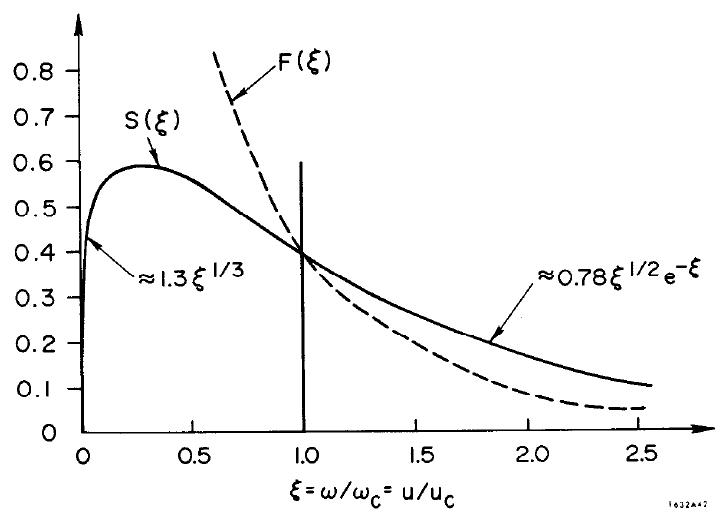
\includegraphics[width=0.7\linewidth]{./Figuras/fig42.jpeg}
	\caption{Espectro de potência normalizado $S$ e espectro do número de fótons $F$ da radiação síncrona. Retirado de \cite{sands1970physics}.}
	\label{fig:fig42}
\end{figure}

O espectro de potência $\mathscr{P}(\omega)$ é obtido a partir de $S(\xi)$ pela equação \eqref{eq:5.2}. Não esqueça que tanto $P_\gamma$ -- veja a equação \eqref{eq:4.4} -- quanto $\omega_c$ dependem de $\gamma$ e $\rho$. Fica claro a partir da \autoref{fig:fig42} que a maioria da potência é encontrada em frequências próximas de $\omega_c$ (como $\omega_c$ é $\gamma^2$ vezes maior que o inverso de $\Delta t$ definido antes, as suposições feitas estão justificadas).

É sabido que a radiação eletromagnética na frequência angular $\omega$ é emitida em uma quantidade de energia $u=\hslash \omega$, onde $\hslash$ é a constante de Plank reduzida por $2\pi$ ($\hslash = h/2\pi = 6.85 \times 10^{-16} eVs$). Seja $n(u)du$ o número de quantidade de energia emitida por unidade de tempo com energias entre $u$ e $u+du$. A potência emitida nessa quantidade é $u n(u)du$, a qual deve ser igual a potência emitida no intervalo de frequência $d\omega = du/\hslash$ na frequência $\omega = u/\hslash$, ou seja,
\begin{align}
	un(u)du = \mathscr{P}(u/\hslash)du/\hslash
\end{align}
Tomando $\mathscr{P}(\omega)$ da equação \eqref{eq:5.2}, a função da distribuição quântica pode ser escrita como
\begin{align}
	n(u) = \frac{P_\gamma}{u_c^2}F\left(\frac{u}{u_c}\right)
\end{align}
com
\begin{align}
	u_c = \hslash \omega_c = \frac{3}{2}\frac{\hslash c \gamma^3}{|\rho|}\label{eq:5.9}\\
	F(\xi) = \frac{1}{\xi}S(\xi)
\end{align}
Como o espectro de frequência, o espectro quântico é, a menos de um fator de escala $P_\gamma/u_c^2$, uma função universal de relação $u/u_c$.

A função $F(\xi)$ também é representada na \autoref{fig:fig42}. A taxa de emissão quântica por unidade de intervalo de energia diverge em pequenas energias\footnote{O espectro é, de qualquer forma, questionável para $u<u_c/\gamma^3$, de acordo com as condições mencionadas anteriormente}. Mas apenas como $u^{-2/3}$, então a taxa de emissão em qualquer intervalo finito de energias quânticas -- uma integral em $u$ -- é finita.

Seja $\mathscr{N}$ a taxa total de emissão quântica (para todas as energias):
\begin{align}
	\mathscr{N} = \int\limits_{0}^{\infty}n(u)du
\end{align}
A partir das expressões assintóticas para $S(\xi)$ na equação \eqref{eq:5.6}, uma integral completa é aproximadamente 1. Na verdade, seu valor exato é $15\sqrt{3}/8$, então
\begin{align}
	\mathscr{N} = \frac{15\sqrt{3}}{8}\frac{P_\gamma}{u_c}\label{eq:5.12}
\end{align}
A energia quântica média é definida como
\begin{align}
	\mean{u} = \frac{1}{\mathscr{N}}\int\limits_{0}^{\infty}un(u)du
\end{align}
A integral é apenas $P_\gamma$, então a energia quântica média é
\begin{align}
	\mean{u} = \frac{8}{15\sqrt{3}}u_c = (0.32...)u_c
\end{align}
Falando grosseiramente, pode-se dizer que a radiação é emitida em quantidades de energia em torno de $u_c$, e com uma taxa média em torno de $P_\gamma/u_c$. Para um elétron com 1GeV movendo-se em uma trajetória com raio de curvatura de 5m,
\begin{align*}
	P_\gamma =& 1.7 \times 10^11\ eVs^{-1}\\
	u_c =& 437\ eV\\
	\mathscr{N} =& 3.2 P_\gamma/u_c = 1.3 \times 10^9\ s^{-1}
\end{align*}

É interessante notar que o número médio de quantidade de energia emitida por radiano da trajetória depende apenas da energia do elétron. Isto é, de fato, quase igual a apenas multiplicar $\gamma$ pela constante estrutural:
\begin{align}
	n\acute{u}mero\ m\acute{e}dio\ de\ energia\ qu\hat{a}ntica\ emitida\ por\ radiano = \frac{5}{2\sqrt{3}}\frac{\gamma}{137}
\end{align}
Para um elétron de 1GeV, o número é em torno de 20. O número real em qualquer intervalo de tempo flutua seguindo uma distribuição Poisson correspondente ao número médio. Portanto, em pequenos números, as flutuações são significativas.

Será visto depois que a excitação quântica das oscilações de um elétron em um anel de armazenamento depende não apenas da taxa média de emissão quântica, mas também da média quadrada da energia quântica. Deve-se esperar que $\mean{u^2}$ seja em torno de $u_c^2$; o que, de fato, é. Analisando detalhadamente, pode-se chegar que
\begin{align}
	\mean{u^2} = \frac{11}{22}u_c^2
\end{align}
Uma quantidade que irá entrar na excitação quântica das oscilações é, de fato, o produto entre a média quadrada da energia quântica e a taxa média $\mathscr{N}$; ou seja,
\begin{align}
	\mathscr{N}\mean{u^2} = \int\limits_{0}^{\infty}u^2n(u)du\label{eq:5.17}
\end{align}
Utilizando a equação \eqref{eq:5.12}, será conveniente escrever
\begin{align}
	\mathscr{N}\mean{u^2} = C_u u_c P_\gamma\label{eq:5.18}
\end{align}
com
\begin{align}
	C_u = \frac{55}{24\sqrt{3}} = 1.32...
\end{align}

É importante manter em mente que tanto $u_c$ quanto $P_\gamma$ são funções da energia do elétron e do raio de curvatura local da trajetória. Tomando $u_c$ da equação \eqref{eq:5.9} e $P_\gamma$ da equação \eqref{eq:4.4},
\begin{align}
	\mathscr{N}\mean{u^2} = \frac{3C_u C_\gamma}{4\pi}\frac{\hslash c^2}{(mc^2)^3}\frac{E^7}{\rho^3} = \frac{55}{24\sqrt{3}}r_e \hslash mc^4 \frac{\gamma^7}{|\rho^3|}
\end{align}
Para um raio de curvatura fixo, a excitação quântica varia com a sétima potência da energia!
	\subsection{Flutuações de energia}\label{sec:5.2}
Hora de examinar os efeitos da emissão quântica sobre as oscilações de energia de um elétron armazenado. Quando uma quantidade de energia é emitida, a energia do elétron subitamente decresce de uma quantidade $u$. Este distúrbio impulsivo causa uma pequena oscilação de energia. O efeito cumulativo de várias distorções -- ocorrendo em tempos aleatórios -- faz com que a oscilação de energia cresça (como em um caminho aleatório). O crescimento é limitado -- na média -- pelo amortecimento; e, em condições estacionárias, as oscilações de energia de um elétron em particular irão flutuar em torno de uma amplitude média. Estas flutuações de energia serão analisadas agora.

Em um primeiro momento, apenas será considerada a medida típica da oscilação de energia -- ou seja, a raiz quadrada média do desvio da energia média -- sem considerar detalhadamente a distribuição de probabilidade do desvio de energia. A natureza desta distribuição será considerada depois.

Na \autoref{sec:3.5} foram analisadas as pequenas oscilações do desvio de energia de um elétron armazenado. Na ausência de distúrbios, e ignorando por agora o amortecimento, o desvio de energia $\epsilon$ é descrito por
\begin{align}
	\epsilon = A_0 e^{i\Omega(t-t_0)}
\end{align}
onde $\Omega$ é a frequência síncrotron (real) e a amplitude $A_0$ é um número real. Agora, suponha que em algum instante $t_i$ a energia subitamente decresça de uma quantidade $u$ -- por emissão quântica. Depois de $t_i$ a energia será como
\begin{align}
	\epsilon = A_0 e^{i\Omega(t-t_0)} - ue^{i\Omega(t-t_i)}
\end{align}
Veja a \autoref{fig:fig43}. Esta nova oscilação pode ser escrita como
\begin{align}
	\epsilon = A_1e^{i\Omega(t-t_1)}
\end{align}
onde
\begin{align}
	A_1^2 = A_0^2 + u^2 - 2A_0u\ cos(\Omega (t_i-t_0))
\end{align}
e $t_1$ é algum deslocamento de tempo que não importa agora.

\begin{figure}[!htb]
	\centering
	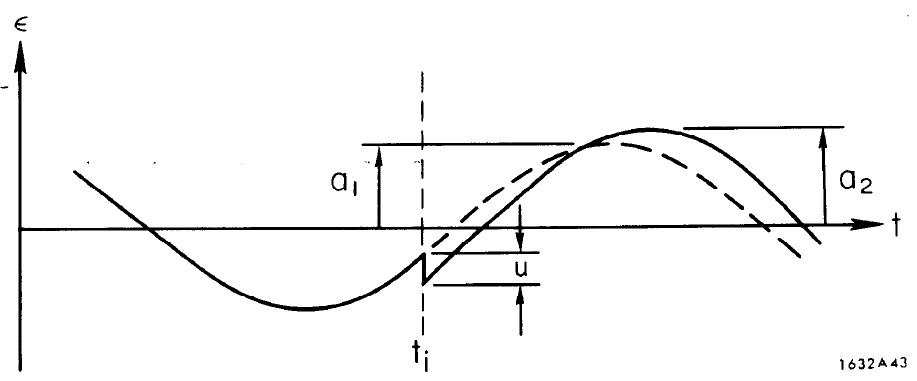
\includegraphics[width=0.9\linewidth]{./Figuras/fig43.jpeg}
	\caption{Efeito nas oscilações de energia devido à emissão de uma quantidade de energia $u$. Retirado de \cite{sands1970physics}.}
	\label{fig:fig43}
\end{figure}

\begin{proof}
	Seja $\epsilon$ dado por
	\begin{align*}
		\epsilon = A_0 e^{i\Omega(t-t_0)} - ue^{i\Omega(t-t_i)}
	\end{align*}
	Fazendo o produto dele pelo seu conjugado, tem-se que
	\begin{align*}
		\epsilon \epsilon^* &= [A_0 e^{i\Omega(t-t_0)} - ue^{i\Omega(t-t_i)}][A_0 e^{-i\Omega(t-t_0)} - ue^{-i\Omega(t-t_i)}]\\
							&= A_0^2 + u^2 - A_0 u[e^{i\Omega(t_i-t_0)} + e^{-i\Omega(t_i-t_0)}]
	\end{align*}
	Pela fórmula de Euler, pode-se transformar as exponencias em senos e cossenos:
	\begin{align*}
		e^{i\Omega(t_i-t_0)} + e^{-i\Omega(t_i-t_0)} &= cos(\Omega(t_i-t_0)) + i\ sen(\Omega(t_i-t_0)) + cos(-\Omega(t_i-t_0)) + i\ sen(-\Omega(t_i-t_0))\\
		&= 2cos(\Omega(t_i-t_0))
	\end{align*}
	Logo,
	\begin{align*}
		\epsilon \epsilon^* = A_0^2 + u^2 - 2A_0u\ cos(\Omega(t_i-t_0))
	\end{align*}
	Agora, deseja-se escrever $\epsilon$ na forma $A_1e^{i\Omega(t-t_1)}$. A partir desta definição, pode-se novamente realizar o produto de $\epsilon$ pelo seu conjugado:
	\begin{align*}
		\epsilon \epsilon^* &= A_1^2\\
		\therefore A_1^2 = A_0^2 + u^2 &- 2A_0u\ cos(\Omega(t_i-t_0))
	\end{align*}
	c.q.d.
\end{proof}

A emissão quântica altera a amplitude da oscilação para um novo valor que depende da amplitude inicial e de $(t_i-t_0)$. Já que o tempo $t_i$ onde uma emissão quântica ocorre é totalmente imprevisível -- e apenas o efeito cumulativo destes eventos interessa -- apenas questões estatísticas são relevantes. Por exemplo: qual a provável mudança de amplitude? Em geral, a fase $(t_i-t_0)$ é completamente aleatória e o valor esperado de $cos(\Omega(t_i-t_0))$ é, portanto, zero. Então a mudança de amplitude provável devido à radiação quântica é
\begin{align}
	\mean{\delta A^2} = \mean{A_1^2 - A_0^2} = u^2
\end{align}
Note que este resultado diz que a mudança provável em $A^2$, a qual ocorre quando é adicionado um novo incremento de oscilação de amplitude $u$ com fase aleatória, é apenas $u^2$ -- o mesmo resultado que seria obtido para $\delta A^2$ se a análise tivesse começado com $A=0$.

Suponha agora que estes eventos quânticos ocorrem em uma sequência de tempo aleatória com uma taxa média $\mathscr{N}$ (número por unidade de tempo). Cada evento muda $A^2$ por uma quantidade $u^2$; e, já que o tempo médio entre cada evento é $1/\mathscr{N}$, espera-se que
\begin{align}
	\mean{\frac{dA^2}{dt}} = \mathscr{N}u^2
\end{align}
Mas a provável taxa de variação de $A^2$ é igual a taxa de variação do valor provável de $A^2$, então
\begin{align}
	\frac{d\mean{A^2}}{dt} = \mathscr{N}u^2\label{eq:5.27}
\end{align}

Além de excitar as oscilações de energia, as perdas de energia discretas contribuem para uma mudança cumulativa na energia. No entanto, estes efeitos médios já foram considerados anteriormente. Seu efeito é produzir as oscilações de energia bem como causar o amortecimento exponencial da amplitude $A$ com uma constante de tempo $\tau_\epsilon = 1/\alpha_\epsilon$. Com este amortecimento, a amplitude decresce a uma taxa $A/\tau_\epsilon$; ou seu quadrado com uma taxa $2A^2/\tau_\epsilon$. A amplitude provável deve ser decrescida pelo amortecimento de forma similar, o que contribuiria à taxa de variação de $\mean{A^2}$ a quantidade
\begin{align}
	\frac{d\mean{A^2}}{dt} = -2\frac{\mean{A^2}}{\tau_\epsilon}\label{eq:5.28}
\end{align}
Quando tanto a excitação quântica quanto o amortecimento estão agindo -- e outras condições estão em estado estacionário -- a soma das taxas das equações \eqref{eq:5.27} e \eqref{eq:5.28} deve ser zero. Logo, encontra-se que o valor provável de $A^2$ é dado por
\begin{align}
	\mean{A^2} = \frac{1}{2}\tau_\epsilon \mathscr{N}u^2
\end{align}
Para oscilações de energia senoidais, o valor esperado de $\epsilon$ é zero, e do seu quadrado -- o qual pode-se chamar de $\sigma_\epsilon^2$ -- é apenas $1/2$ vezes o valor provável do quadrado da amplitude:
\begin{align}
	\sigma_\epsilon^2 = \mean{\epsilon^2} = \frac{\mean{A^2}}{2} = \frac{1}{4}\tau_\epsilon \mathscr{N} u^2\label{eq:5.30}
\end{align}
Desta forma, seria a média do quadrado da flutuação de energia na oscilação de energia que seria produzida pelas emissões quânticas aleatórias, todas de mesma energia $u$. Isto deve corresponder aproximadamente às flutuações de energia em um anel de armazenamento se $u$ fosse a energia quântica típica $u_c$ e $\mathscr{N}$ fosse a taxa média $P_\gamma/u_c$.

Um resultado equivalente aproximado pode ser obtido a partir de um simples argumento. A flutuação de energia típica vem do desvio da média do número de quantidade de energia emitida em um intervalo de amortecimento $\tau_\epsilon$. A média do número emitido é $\mathscr{N}\tau_\epsilon$, então o desvio RMS da média é $\sqrt{\mathscr{N}\tau_\epsilon}$ (distribuição de Poisson). Já que cada partícula quântica tem energia em torno de $u_c$, na média,
\begin{align}
	\sigma_\epsilon \approx \sqrt{\mathscr{N}\tau_\epsilon}u_c
\end{align}
Este resultado é parecido com o que foi obtido na equação \eqref{eq:5.30}. Note que, como $\mathscr{N} \approx P_\gamma/u_c$ e $\tau_\epsilon \approx E_0/P_\gamma$, também pode-se escrever
\begin{align}
	\sigma_\epsilon \approx \sqrt{E_0 u_c}\label{eq:5.32}
\end{align}
Concluindo: a flutuação de energia é aproximadamente a média geométrica entre a energia do elétron e a energia crítica do fóton!

Pode-se, então, fazer um cálculo mais preciso -- o qual é um pouco mais complicado. Primeiro, porque existe uma distribuição estatística do tamanho das quantidades de energia. Segundo, porque tanto a distribuição quanto a taxa média podem variar ao longo do anel. Retornando à equação \eqref{eq:5.27}, deve-se considerar separadamente a contribuição de cada intervalo de tamanhos quânticos a $d\mean{A^2}/dt$. Estas quantidades com energias entre $u$ e $u+\Delta u$ -- onde existem $n(u)\Delta u$ quantidades de energia emitidas por unidade de tempo -- irão contribuir com
\begin{align}
	\Delta \left\{\frac{d\mean{A^2}}{dt}\right\} = u^2 n(u) \Delta u
\end{align}
Mas como a emissão quântica em várias energias não são correlacionadas, cada energia irá contribuir de forma independente ao crescimento aleatório de $\mean{A^2}$. Então basta somar as contribuições de cada intervalo $\Delta u$:
\begin{align}
	\frac{d\mean{A^2}}{dt} = \int\limits_{0}^{\infty}u^2n(u)du
\end{align}
Esta integral já foi analisada: é apenas $\mathscr{N}\mean{u^2}$ (equação \eqref{eq:5.17}). Logo,
\begin{align}
	\frac{d\mean{A^2}}{dt} = \mathscr{N}\mean{u^2}
\end{align}

A taxa de crescimento obtida depende da energia do elétron -- a qual pode ser avaliada como a energia nominal $E_0$ -- e do raio local de curvatura da trajetória $\rho$, ambos os quais podem variar ao longo do anel. Da derivação feita, pode-se esperar que o tempo para haver uma variação "significante" na amplitude da oscilação de energia será da ordem da constante de tempo de amortecimento $\tau_\epsilon$. Como tanto o período de oscilação $\approx 1/\Omega$ quanto o tempo de amortecimento $\tau_\epsilon$ são muito maiores que o período de uma revolução $T_0$, pode-se substituir a rápida variação $\mathscr{N}\mean{u^2}$ pelo seu valor médio em uma revolução no anel. Também pode-se criar um erro desprezível (na média) ao substituir o raio de curvatura instantâneo da trajetória $\rho$ em cada azimutal $s$ pelo raio local de curvatura na órbita ideal. Tomando a média de $\mathscr{N}\mean{u^2}$ em uma revolução integrando com respeito à coordenada azimutal $s$, pode-se definir
\begin{align}
	Q_\epsilon = \mean{\mathscr{N}\mean{u^2}}_s = \frac{1}{2\pi R}\oint\mathscr{N}\mean{u^2}ds
\end{align}
Seguindo o resto da derivação como foi feito anteriormente, obtém-se para o quadrado da média da flutuação de energia:
\begin{align}
	\sigma_\epsilon^2 = \frac{1}{4}\tau_\epsilon Q_\epsilon\label{eq:5.37}
\end{align}

Este resultado pode parecer bem simples, porém as complicações estão escondidas nos termos $\tau_\epsilon$ e $Q_\epsilon$. Primeiro, para analisar $Q_\epsilon$, é preciso avaliar $\mathscr{N}\mean{u^2}$ na órbita ideal. Começando com a forma derivada na equação \eqref{eq:5.18}, pode-se obter $P_\gamma$ na órbita ideal a partir da equação \eqref{eq:4.4} fazendo $E=E_0$ e $1/\rho = G$ (veja a \autoref{sec:2.2}), então
\begin{align}
	\left(P_\gamma\right)_{\acute{o}rbita\ ideal} = \frac{c C_\gamma}{2\pi}E_0^4G^2
\end{align}
o que pode ser reescrito -- utilizando a equação \eqref{eq:4.9} -- como
\begin{align}
	\left(P_\gamma\right)_{\acute{o}rbita\ ideal} = \frac{\mean{P_\gamma}_s G^2}{\mean{G^2}_s}
\end{align}
E $u_c$ na órbita ideal pode ser obtida pela equação \eqref{eq:5.9}:
\begin{align}
	\left(u_c\right)_{\acute{o}rbita\ ideal} = \frac{3}{2}\hslash c \gamma_0^3 |G|\label{eq:5.40}
\end{align}
Logo, tem-se que
\begin{align}
	\left(\mathscr{N}\mean{u^2}\right)_{\acute{o}rbita\ ideal} = C_u \frac{3}{2}\hslash c \gamma_0^3 |G| \frac{\mean{P_\gamma}_s G^2}{\mean{G^2}_s}\label{eq:5.41}
\end{align}
A única quantidade que varia ao longo da órbita ideal é $G$, então $Q_\epsilon$ pode ser escrito como\footnote{Abandona-se o subscrito $s$ na média sobre o anel pois já está claro que todas as quantidades mostradas estão sendo analisadas sobre $s$. Por exemplo, $\mean{G^2}$ significa $\oint G^2(s)ds/ L$ onde $L$ é o comprimento da órbita.}
\begin{align}
	Q_\epsilon = \frac{3}{2}C_u\hslash c \gamma_0^3 \frac{\mean{P_\gamma} \mean{|G^3|}}{\mean{G^2}}
\end{align}
Tomando $\tau_\epsilon$ da equação \eqref{eq:4.53},
\begin{align}
	\tau_\epsilon = \frac{E_0}{J_\epsilon\mean{P_\gamma}}
\end{align}
pode-se finalmente reescrever a equação como
\begin{align}
	\sigma_\epsilon^2 = \frac{3 C_u \hslash m c^3\ \gamma_0^4\ \mean{|G^3|}}{4 J_\epsilon \mean{G^2}}
\end{align}

O desvio padrão de energia relativo $\sigma_\epsilon/E_0$ é normalmente mais significante. Pode-se escrevê-lo como
\begin{align}
	\left(\frac{\sigma_\epsilon}{E_0}\right)^2 = \frac{C_q \mean{|G^3|} \gamma_0^2}{J_\epsilon \mean{G^2}}\label{eq:5.45}
\end{align}
com $C_q$ -- a qual é chamada de constante quântica -- dada por
\begin{align}
	C_q = \frac{3C_u\hslash}{4mc} = \frac{55}{32\sqrt{3}}\frac{\hslash}{mc} = 3.84\ \times\ 10^{-13}\ m\label{eq:5.46}
\end{align}
É muito próxima do comprimento de onda Compton do elétron.

O termo $|G^3|/J_\epsilon \mean{G^2}$ é uma propriedade geométrica do campo guia. Mais especificamente,
\begin{align}
	\frac{\mean{|G^3|}}{J_\epsilon\mean{G^2}} = \frac{1}{J_\epsilon}\frac{\oint |G^3(s)|ds}{\oint G^2(s)ds}
\end{align}
É aproximadamente igual ao inverso do raio de curvatura "típico" da órbita ideal. O resultado da equação \eqref{eq:5.45} é então aproximadamente $\gamma^2$ vezes a relação entre o comprimento de onda de Compton e o raio da órbita. Para qualquer anel, o espalhamento quântico induzido no desvio de energia relativo ($\sigma_\epsilon/E_0$) varia de forma diretamente proporcional à energia do elétron.

Em um anel de armazenamento com campo guia isomagnético, a expressão geométrica acima é apenas $1/J_\epsilon \rho_0$, e
\begin{align}
	\left(\frac{\sigma_\epsilon}{E_0}\right)^2 = \frac{C_q \gamma_0^2}{J_\epsilon \rho_0}\ \ (isomag.)\label{eq:5.48}
\end{align}
Em um anel de armazenamento isomagnético com 5m de raio de curvatura, elétrons armazenados com 1 GeV de energia irão ter um desvio de energia próximo a 0.04\% da energia -- ou em torno de 40 keV.
	\pagebreak


\bibliography{biblio}


\end{document}








